\documentclass{xdupgthesis}

% XDUTS核心配置
\xdusetup{
  style = {
    customize-los = false,
    customize-loa = false,
  },
  info = {
    graduate-type         = 硕士,
    degree-type           = 专业,
    % 核心必填信息
    title                 = {面向单向双车道高速公路的多地磁传感器车辆目标跟踪方法研究},
    title*                = {Research on Vehicle Target Tracking Methods Using Multiple Geomagnetic Sensors for Unidirectional Two-Lane Expressways},
    author                = {侯照莹},
    author*               = {Zhaoying Hou},
    department            = {通信工程学院},
    major                 = {信息与通信工程},
    major*                = {Information and Communication Engineering},
    sub-major             = {通信计算融合与场景应用},
    student-id            = {23011210459},
    supervisor            = {毛国强},
    supervisor*           = {Guoqiang Mao},
    supv-title            = {教授},
    supv-title*           = {Professor},
    supervisor-enterprise = {},
    supervisor-enterprise*= {},
    supv-ent              = {},
    supv-ent*             = {},
    supv-ent-title        = {},
    supv-ent-title*       = {},
    supervisor-title      = {教授},
    supervisor-title*     = {Professor},
    supervisor-enterprise-title  = {},
    supervisor-enterprise-title* = {},
    % 学科与保密信息
    domain                = {新一代电子信息技术（含量子技术等）},
    clc                   = {TP391.41},
    secret-level          = {公开},
    submit-date           = {2026-03-01},
    % 关键词
    keywords              = {车辆目标跟踪，地磁传感器，卡尔曼滤波，数据关联，在线聚类},
    keywords*             = {Vehicle Target Tracking, Geomagnetic Sensor, Kalman Filtering, Data Association, Online Clustering},
    % 附件与声明文件
    abstract              = {chapters/abstract-zh.tex},
    abstract*             = {chapters/abstract-en.tex},
    acknowledgements      = {chapters/acknowledgements.tex},
    bio                   = {chapters/biography.tex},
    appendix              = {chapters/appendix1.tex},
    statement-scan        = {},
    statement-sign        = {},
    los                   = {chapters/los.tex},
    loa                   = {chapters/loa.tex},
    % 参考文献
    bib-resource          = {references.bib},
  }
}

% -------------------------
% 常用包（按功能分组）
% -------------------------
\usepackage{graphicx}
\graphicspath{{images/}}

\usepackage{amsmath}
\usepackage{amsfonts}
\usepackage{amssymb}

\usepackage{booktabs}
\usepackage{multirow}
\usepackage{makecell}
\usepackage{tabularx}
\usepackage{threeparttable}

\usepackage{subcaption}

\usepackage{xcolor}
\usepackage{pifont}

\usepackage{enumitem}


\usepackage{graphicx}
\graphicspath{{E:/MyLunWen/xduts-main/code/chapter4/experiment123/result/}}
 \usepackage{booktabs}
 \usepackage{float}

% 浮动体控制（你已在用：建议保留）
\usepackage[section]{placeins} % 提供 \FloatBarrier，并阻止浮动体跨 section
\usepackage{flafter}          % 防止浮动体出现在源码位置之前

% 超链接与智能引用：hyperref 必须在 cleveref 前面
\usepackage{hyperref}
\usepackage{cleveref}

% -------------------------
% 全局宏：模型名（你原本就有）
% -------------------------
\newcommand{\ModelTF}{GazeFusion}
\newcommand{\ModelMM}{GazeGuide}

% -------------------------
% 全局宏：地磁章节统一口径（按你第2章需要）
% -------------------------
\newcommand{\Fs}{\ensuremath{50\,\mathrm{Hz}}}
\newcommand{\MagUnit}{\ensuremath{\mathrm{nT}}}
\newcommand{\SmoothLen}{\ensuremath{7}}        % L_s
\newcommand{\BgWinPts}{\ensuremath{500}}       % N_0 (10 s @ 50 Hz)
\newcommand{\ProbFloor}{\ensuremath{10^{-6}}}  % p_min

% 兜底：即使 placeins 被注释掉，也不至于 \FloatBarrier 报错
\providecommand{\FloatBarrier}{}

% -------------------------
% 文档开始
% -------------------------
\begin{document}


\chapter{绪论}

\section{研究背景与意义}

随着我国跨区域人员流动日益频繁和公路货运需求持续增长，高速公路在综合交通运输体系中的支撑作用不断增强。交通运输部数据显示，截至2024年末我国高速公路里程已达19.07万公里\cite{mot2024statisticalbulletin}，路网规模的持续扩展也使高速公路运行管理由单纯保障通行，逐步转为面向安全、效率与韧性的精细化治理。尤其在高速场景下，车辆运行速度高、交通流密度大、扰动传播快，局部异常往往会迅速影响车道乃至路段整体运行状态。因此，如何构建面向高速路段的持续感知与精细管理能力，已成为保障路网安全高效运行、提升运行韧性并支撑主动交通管理的重要基础问题。

在此背景下，智能交通系统（Intelligent Transportation Systems, ITS）通过交通检测与监视、通信与信息处理等技术实现对交通状态的实时感知与服务支撑，从而为交通管理与控制提供数据基础\cite{mimbela2007vdstits}。随着交通治理由以流量、平均速度等宏观统计指标为主，逐步转向对车道级运行机理与驾驶行为的微观刻画，车辆轨迹数据因能够连续表征车辆的时空运动过程，已成为交通分析、预测与控制的关键数据形态\cite{liu2025trajectorysurvey}，并可用于拥堵成因诊断、行驶安全风险与冲突指标计算，以及车路协同控制策略评估等任务。但连续车辆轨迹并不是路侧传感器的直接输出，而是需要在离散检测结果基础上完成关联、状态估计与身份延续后才能形成，因此，车辆目标跟踪成为连接路侧感知与轨迹级应用的关键环节。目标跟踪的核心任务是将离散量测在时间轴上持续关联为可更新的车辆轨迹，并尽量保持位置与速度估计的连续性，为行为分析提供可靠输入，以支撑车道级速度估计、时距演化分析和变道行为识别等应用。需要指出的是，车辆目标跟踪的实施效果高度依赖路侧感知载体的观测能力与工程可用性，不同类型传感器在目标分辨能力、环境适应性以及部署维护成本等方面各有特点，这也决定了其在高速公路场景中的适用边界。以常见路侧传感器为例，摄像头能够提供丰富的轮廓、纹理与颜色信息，但在强逆光、夜间、雨雾等条件下检测质量易波动\cite{Pandharipande2023Perception}；激光雷达空间分辨率高、测距精度较好，但设备成本较高，且在降雨、降雪等天气下点云质量可能受到影响\cite{Pandharipande2023Perception,Wu2025LiDARAdverseWeather}；毫米波雷达对光照不敏感，在恶劣天气下相对更稳健，但在强多径环境中仍可能出现虚假检测，且受角分辨率限制，对邻近目标的分离能力仍存在约束\cite{Kong2025mmWaveSurvey}。

在面向大范围、全天候部署的路侧感知体系中，地磁传感器因成本较低、体积小、安装灵活且对光照与气象条件不敏感，被认为是面向低成本规模化部署的关键候选方案，其基本机理是车辆等铁磁体通过时会扰动局部地球静磁场，传感器对磁场变化进行采样与特征提取，从而输出车辆通过事件及相关磁特征\cite{culik2023wirelessmagnetic}。与能够直接给出连续轨迹的感知方式不同，多地磁传感器组网条件下得到的是跨位置的离散检测数据流，这些数据需要在时间轴上对齐，并在多车并行与变道交互条件下完成跨点匹配与身份维护，才能转化为可用于微观分析的连续轨迹。但在实际部署中，多地磁传感器跟踪系统存在数据随机延迟到达、漏检以及噪声干扰等非理想因素的影响，同时由于车辆行驶行为复杂，邻道干扰与双车长距离并行通过在上报量测的时空特性上又具有较强相似性，难以简单依据单条量测特征判断区分，从而影响车辆实时跟踪的准确性与稳定性。进一步地，系统连续多年使用后，部分地磁传感器还可能因器件老化而检测能力下降，连续漏检现象增多，使跟踪结果更易出现轨迹碎片化\cite{rakai2022dataassociation,feng2021magneticdataassociation,wang2023distributedmagnetic}。由此可见，如何在不完美量测条件下实现多地磁事件流的稳健在线跟踪，并在长缺测条件下进一步恢复断裂轨迹片段、保持轨迹身份一致性，是发挥地磁传感技术在高速运行监测中应用价值的关键技术问题，也对轨迹级安全评估与精细化交通管理具有重要意义。

\section{国内外研究现状}

\subsection{地磁传感器车辆检测研究现状}
地磁传感器是一种基于环境磁场变化的路侧检测设备，通常采用磁阻器件对周围磁场进行连续采样。当车辆驶过传感器附近时，车辆所含铁磁材料会对局部磁场分布产生扰动，使磁信号在幅值与形态上出现显著变化；对该扰动信号进行检测与判别即可实现车辆通过事件的识别\cite{balid2018intelligent,feng2022magmonitor}。

早期研究主要关注单点条件下的车辆检出与过车时刻提取。Haoui 等以无线地磁检测系统 VDS240 为例，给出了由地磁传感器完成车辆存在判定以及车辆到达、离开时刻提取，再由中心侧汇聚处理的基本流程\cite{haoui2008wirelessmagnetic}。为提高检测在复杂工况下的稳定性，Markevičius等根据磁场分量在车辆接近和通过传感器时呈现的状态变化提出车辆检测思路，指出车辆相对地磁传感器的通过轨迹差异会显著改变扰动波形形态，因此检测阶段通常需要结合归一化与自适应处理，以减弱同一车辆因通过位置不同带来的特征漂移\cite{markevicius2016dynamic}。在车辆通过检测逐步稳定后，研究开始从检测记录中进一步估计速度、车长等交通参数。Taghvaeeyan与Rajamani提出由多个地磁传感器组成的便携式路侧磁传感系统，利用纵向间隔布设的地磁传感器互相关估计车速，并结合过车持续时间与速度推断车辆磁长度，同时利用横向布设信息抑制相邻车道大型车辆引起的误触发\cite{taghvaeeyan2014portable}。Balid等进一步将车辆检测、速度估计、长度估计、车辆分类和时间同步等功能集成到智能无线地磁传感器中，并通过实地测试验证了端侧实时处理的可行性\cite{balid2018intelligent}。另一方面，为了在单个地磁传感器上提取更丰富的信息，Feng等提出MagMonitor。该方法虽然在车辆磁场建模中采用了多磁偶极描述，但观测端仍是单个地磁传感器，其目标是在单传感器条件下实现速度估计与车辆分类，说明模型化描述有助于提升单个地磁传感器检测输出的稳定性与可解释性\cite{feng2022magmonitor}。当研究进一步扩展到阵列观测时，Amodio等利用路面多地磁传感器记录车辆不同部位的多段磁响应，并采用动态时间规整实现车辆型号识别与横向通过位置估计，说明空间采样能够支持更细粒度的车辆通过特性刻画\cite{amodio2021vehiclemodel}。在此基础上，Kwong等进一步利用两处地磁传感器获得的带噪磁响应与过车时刻进行车辆重识别，实现了路段旅行时间估计，说明地磁响应不仅可用于本地检测，也可作为跨点匹配线索\cite{kwong2009arterialtravel}。

总体来看，现有研究已经从单点车辆通过检测，逐步扩展到速度、占有率、车长和车辆分类等参数估计；在多地磁传感器阵列条件下，还能够进一步识别车型、估计车辆横向通过位置，并支撑跨点重识别。相比之下，面向多地磁传感器组网的车辆跟踪研究仍相对有限。单点检测中的基线漂移、波形波动和误触发抑制已有较多讨论，但当系统扩展到多地磁传感器协同观测后，不同地磁传感器之间的时钟偏差、随机通信延迟、漏检以及噪声干扰导致的虚警会进一步放大跨点对应难度。Feng等指出，地磁传感器之间的时钟偏差与换道会引起量测时标错位以及漏检、重复检出，从而增加多点关联难度\cite{feng2021magneticdataassociation}。Mao等进一步讨论了随机延迟与不准确检测条件下的异步融合问题，并在融合毫米波雷达与地磁量测的场景中验证了方法有效性；但对于仅依赖地磁量测、且量测可能出现更多连续漏检的低成本高速路侧部署条件，上述思路仍难以直接满足在线跟踪需求\cite{mao2025asynchronousfusion}。因此，在复杂环境下融合多地磁传感器量测，实现多车辆实时跟踪并保持轨迹连续性与身份一致性，仍是亟待解决的关键问题。

\subsection{滤波算法研究现状}
滤波算法是多目标跟踪的核心步骤之一，用于实现跟踪目标的运动状态预测与更新。之所以需要采用滤波算法对目标状态进行估计，是因为目标跟踪过程中通常伴随着测量误差和环境噪声，传感器直接获得的量测往往带有随机波动和不确定性。滤波算法能够结合目标的运动规律与当前观测信息，对含噪量测进行递推修正和平滑处理，从而减弱噪声和误差对估计结果的影响，提高对目标位置、速度等状态量估计的准确性与稳定性\cite{barshalomli1995multitarget}。

从研究脉络来看，滤波方法的发展大体经历了从线性平稳过程到线性动态系统，再到非线性、机动与非高斯场景的逐步扩展。最早可追溯到 Wiener 于 1949 年提出的平稳随机过程最优线性滤波理论\cite{wiener1949extrapolation}。该理论奠定了现代滤波方法的数学基础，不过其主要面向平稳随机过程，求解时往往需要借助 Wiener--Hopf 方程这类用于求解最优滤波器的积分方程，因此在处理状态随时间变化的动态系统时，建模和实时实现都不够方便。随后，Kalman 于 1960 年从状态空间建模和递推估计的角度重新表述滤波与预测问题，提出了 Kalman 滤波算法\cite{kalman1960linearfiltering}。与 Wiener 滤波相比，Kalman 滤波能够以递推方式完成预测和更新，更适合实时状态估计，因此很快成为目标跟踪领域线性系统状态估计的经典方法。随着跟踪对象由近线性目标扩展到更复杂的机动目标，20 世纪 60 年代中期以 Schmidt 为代表的研究开始将状态空间方法系统应用于导航等非线性问题，并逐步形成扩展卡尔曼滤波（Extended Kalman Filter, EKF）的基本思路\cite{schmidt1966statespace}。其做法是在每一步估计时，先在当前估计点附近将非线性状态方程和量测方程近似为线性形式，再沿用 Kalman 滤波的递推框架完成状态估计。由于 EKF 与 KF 在形式上较为接近，工程实现相对方便，因此得到了广泛应用；但当系统非线性较强或模型失配较明显时，这种近似带来的误差容易逐步积累，进而导致估计精度下降，严重时甚至可能出现发散。进一步地，针对机动目标在不同运动模式之间切换的问题，Blom 和 Bar-Shalom 于 1988 年提出了交互式多模型（Interacting Multiple Model, IMM）算法\cite{blom1988imm}，通过并行运行多个运动模型并根据模型概率进行交互和融合，有效缓解了单一运动模型难以刻画加减速、转向或变道等机动行为的问题。进入 20 世纪 90 年代以后非线性滤波研究继续沿两条路线展开。一方面，Gordon 等于 1993 年提出了 Bootstrap 粒子滤波（Bootstrap Particle Filter），其基本思想是用一组带权粒子来近似系统状态的后验分布，使滤波过程不再严格受限于线性和高斯假设\cite{gordon1993bootstrap}。该方法能够处理更一般的非线性、非高斯问题，但也容易受到粒子退化的影响，并且为保证估计精度通常需要较多粒子样本，从而带来较高的计算代价。另一方面，Julier 和 Uhlmann 在 1997 年提出了无迹卡尔曼滤波（Unscented Kalman Filter, UKF），并在 2004 年对无迹变换与无迹滤波进行了系统总结\cite{julier1997ukf,julier2004unscented}。UKF 通过选取一组确定性的 Sigma 点来传播均值和协方差，避免了 EKF 中先将非线性方程近似为线性形式的步骤，因此在不少非线性场景下较好地兼顾了实现便利性与估计精度。不过，其本质上仍然是利用有限统计量对后验分布进行近似表示。

总体来看，滤波算法的研究主线已经从早期面向平稳过程的线性最优估计，逐步发展为兼顾非线性、机动模型切换以及非高斯噪声的状态估计框架。对于本文所研究的高速路侧多地磁传感器车辆目标跟踪问题而言，车辆运动模式会随交通状态变化，量测又容易受到环境扰动与漏检的影响，因此如何在保证实时性的前提下兼顾机动性描述能力与估计稳定性，仍是这类滤波方法设计中的重要取舍。

\subsection{数据关联研究现状}
与单目标场景不同，多目标跟踪中的核心难点之一在于量测归属不确定性。滤波预测只能为每条轨迹给出先验分布，而当前时刻的量测究竟应由哪一条轨迹吸收更新，需要通过数据关联判定；一旦发生错误关联，错误量测会进入状态更新，并引发状态漂移与ID切换，且这种误差会在后续递推中持续累积\cite{barshalomli1995multitarget}。

数据关联问题在跟踪理论发展的早期就已受到关注。Singer与Stein在研究量测来源不精确条件下的跟踪滤波问题时指出，关联不确定性会直接影响递推估计的稳定性与可信度\cite{singer1971optimaltracking}。围绕这一问题，较早的研究思路是先依据预测均值与协方差构造验证门，以尽量排除明显不可能的匹配，再在门内选择最可能的关联对象。Sea提出的实时监视系统次优关联方法采用门内最近邻量测进行更新，后续被概括为最近邻数据关联（Nearest Neighbor Data Association, NNDA）\cite{sea1971suboptimal}。这种方法实现简单，适合实时处理，但当目标间距较小或量测较为拥挤时，多个验证门容易重叠，单一扫描内的最近邻选择也更容易产生误配。随着研究深入，数据关联逐步由门内局部选择发展为全局优化与概率化建模两条主要路线。确定性方法在每一帧输出唯一的匹配，典型代表包括NNDA及其全局化形式全局最近邻（Global Nearest Neighbor, GNN），后者通常在门控后的候选集合上求解指派问题，以获得整体代价最小的匹配结果，Kuhn提出的匈牙利算法是其中常用的求解器\cite{kuhn1955hungarian}。这类硬判决方法计算量较小、实现直接，但一旦在拥挤场景中发生误配，往往难以及时修正。为缓解这一问题，Bar-Shalom与Tse提出概率数据关联（Probabilistic Data Association, PDA），通过计算验证门内各候选量测的关联概率并进行加权更新，降低了单一错误匹配对状态估计的冲击\cite{barshalom1975pda}；Fortmann等进一步扩展得到联合概率数据关联（Joint Probabilistic Data Association, JPDA），通过对多目标共享量测的联合关联事件进行概率化处理，减轻了多目标争抢量测时的轨迹黏连问题\cite{fortmann1983jpda}。考虑到JPDA在目标数增加时联合事件枚举开销迅速上升，后续又出现了广义概率数据关联与简化JPDA等近似形式，用于在在线复杂度受限条件下降低计算负担并保持一定的关联精度\cite{pan2005gpda,qin2005simplifiedjpda,sheng2020simplifiedjpda}。进一步地，由于单扫描方法只利用当前时刻的信息，早期误配容易影响后续门控结构并形成链式传播，研究者开始把关联决策从单帧扩展到有限时间窗口内的多帧联合推断。Reid提出多假设跟踪（Multiple Hypothesis Tracking, MHT），通过并行维护多套关联假设来延后决策\cite{reid1979mht}，Cox与Hingorani进一步讨论了高效实现与剪枝策略对实时性的关键作用\cite{cox1996efficientmht}。在此基础上，Murty算法可用于生成多组候选指派\cite{murty1968ranking}，网络流、贪心以及K最短路等全局优化框架也被广泛用于多帧轨迹连接\cite{zhang2008networkflow,pirsiavash2011greedy,berclaz2011kshortest}。

总体来看，数据关联方法已经形成了从门控与单帧决策，到概率化软关联，再到有限时域多帧联合推断的清晰发展脉络。不同方法在实时性、鲁棒性与计算复杂度之间各有取舍，这也为后续面向特定场景的在线跟踪算法设计提供了基础。

\subsection{在线轨迹聚类方法研究现状}
与前述侧重递推滤波与在线关联不同，本节关注当观测出现较长中断或连续缺测时，在线跟踪输出往往分解为多个短轨迹片段，从而出现轨迹碎片化现象。在此背景下，研究重点由单次量测更新转向跨片段的一致性组织，即将轨迹点或轨迹片段作为聚类对象，利用时空邻近与运动一致性线索对同一目标的片段进行增量聚合与归并，以在更长时间尺度上提升轨迹连续性与身份一致性\cite{wang2021trajectorysurvey,wang2024reconstruction}。

从聚类的一般方法出发，密度聚类常被用作基础工具。DBSCAN以密度可达性定义簇结构，能够发现任意形状的簇，并将低密度样本识别为噪声点，因此在噪声与离群点并存的数据中具有较好的结构分离能力\cite{ester1996dbscan}。不过，DBSCAN主要面向静态数据集，难以直接满足数据流场景中一次扫描、有限存储与持续到达的处理约束。面向数据流聚类，CluStream将在线阶段的微簇维护与离线阶段的宏聚类分析相分离，通过维护可更新的统计摘要支持不同时间尺度上的聚类查询，为流式数据的可扩展聚类提供了经典范式\cite{aggarwal2003clustream}。在此基础上，DenStream进一步引入核心微簇、潜在微簇与离群微簇等结构，并结合剪枝策略实现对噪声与演化簇结构的在线处理，使聚类过程在数据分布随时间变化时仍能保持跟踪性与稳健性\cite{cao2006denstream}。总体来看，上述工作形成了由静态密度聚类向演化数据流聚类拓展的基础框架，为后续将轨迹样本视为数据流并进行增量归并提供了方法论支撑。

进一步面向轨迹数据，已有研究指出仅依赖通用点集聚类往往不足以刻画轨迹数据中蕴含的时序信息与运动一致性，从而难以稳定完成片段归并。为此，研究者提出面向轨迹数据流的在线聚类方法，将轨迹点序列转化为具有时序语义的表示单元并进行增量组织。Yu等提出CTraStream，将移动对象的增量轨迹表示为线段流，并结合线段间距离度量与在线更新机制，在流式到达过程中持续形成包含时空信息的轨迹簇，为轨迹数据流的实时模式提取提供了可操作框架\cite{yu2013ctra}。Mao等进一步针对流式轨迹的概念漂移与时空开销约束提出OCluST，通过微聚类与宏聚类两级结构在给定时间跨度内维护轨迹簇，使聚类结果能够随轨迹模式演化而更新，体现了时间窗口内增量聚合的轨迹流聚类思路\cite{mao2018oclust}。此外，面向轨迹重建与行为一致性约束的研究也在持续推进\cite{zhao2024behaviouraloc}。然而，当数据呈现长间隔缺测、目标数量动态变化时，现有在线轨迹聚类方法仍难同时兼顾簇结构的稳定维护与误聚类抑制。




\section{论文研究内容及章节安排}

本文的研究内容是将多地磁传感器车辆检测与目标跟踪技术相结合，面向单向双车道高速路段的地磁检测数据，实现多车辆在线跟踪并输出连续、身份一致的车辆轨迹。全文安排如下：

第一章为绪论，阐述高速公路运行监测与微观过程管控需求，概述地磁感知与车辆跟踪研究现状，明确本文研究问题、技术路线与创新点。
第二章给出单向双车道多地磁布设与量测建模，并介绍车辆检测与事件生成、状态空间模型、贝叶斯递推、门控与数据关联以及轨迹重构相关基础概念，为后续方法推导统一符号与假设。

第三章面向噪声统计不确定、短时漏检与密集交通下的关联歧义，提出变分贝叶斯噪声自适应滤波结合门控与软关联的在线多目标跟踪方法，并给出算法流程与性能分析。

第四章面向连续缺测引发的轨迹碎片化问题，设计基于聚类的轨迹重构策略，对跟踪输出进行二级整合并验证其有效性。第五章总结全文工作与主要结论，讨论研究局限并展望后续改进方向。





\chapter{多地磁传感器车辆目标跟踪理论概述}
\label{ch:ch2_event_detect}

\section{引言}\label{sec:ch2_intro}

在前述研究背景与相关工作综述的基础上，本章围绕单向双车道多地磁传感器部署场景下的车辆目标跟踪问题，对相关理论与部署模型进行系统阐述。具体而言，首先介绍地磁传感器的车辆检测机理及事件生成过程；随后给出本文所采用的系统部署模型及其对应的测量模型；在此基础上，对卡尔曼滤波与数据关联的基本理论进行回顾，并进一步梳理在线聚类算法的相关方法，为后续章节的算法设计与推导奠定理论基础。


\section{地磁传感器检测车辆}\label{sec:ch2_principle}

\subsection{地磁传感器检测车辆原理}\label{sec:ch2_basic}

地磁传感器通过磁阻器件对安装位置处的三轴磁场强度进行连续采样。由于地球磁场在短时间尺度内相对平稳，无车条件下传感器观测通常围绕一条基线缓慢波动。如图~\ref{fig:mag_disturbance}所示，当车辆进入传感器的有效作用范围时，车辆所含铁磁材料会改变局部磁场分布，使三轴磁场观测在幅值与形态上出现明显偏移；车辆驶离后，观测值逐步回到基线附近。由此，车辆通过过程可以抽象为磁场观测相对基线的偏离与回归过程，为车辆检测提供了可观测依据\cite{haoui2008wirelessmagnetic}。

\begin{figure}[htbp]
	\centering
	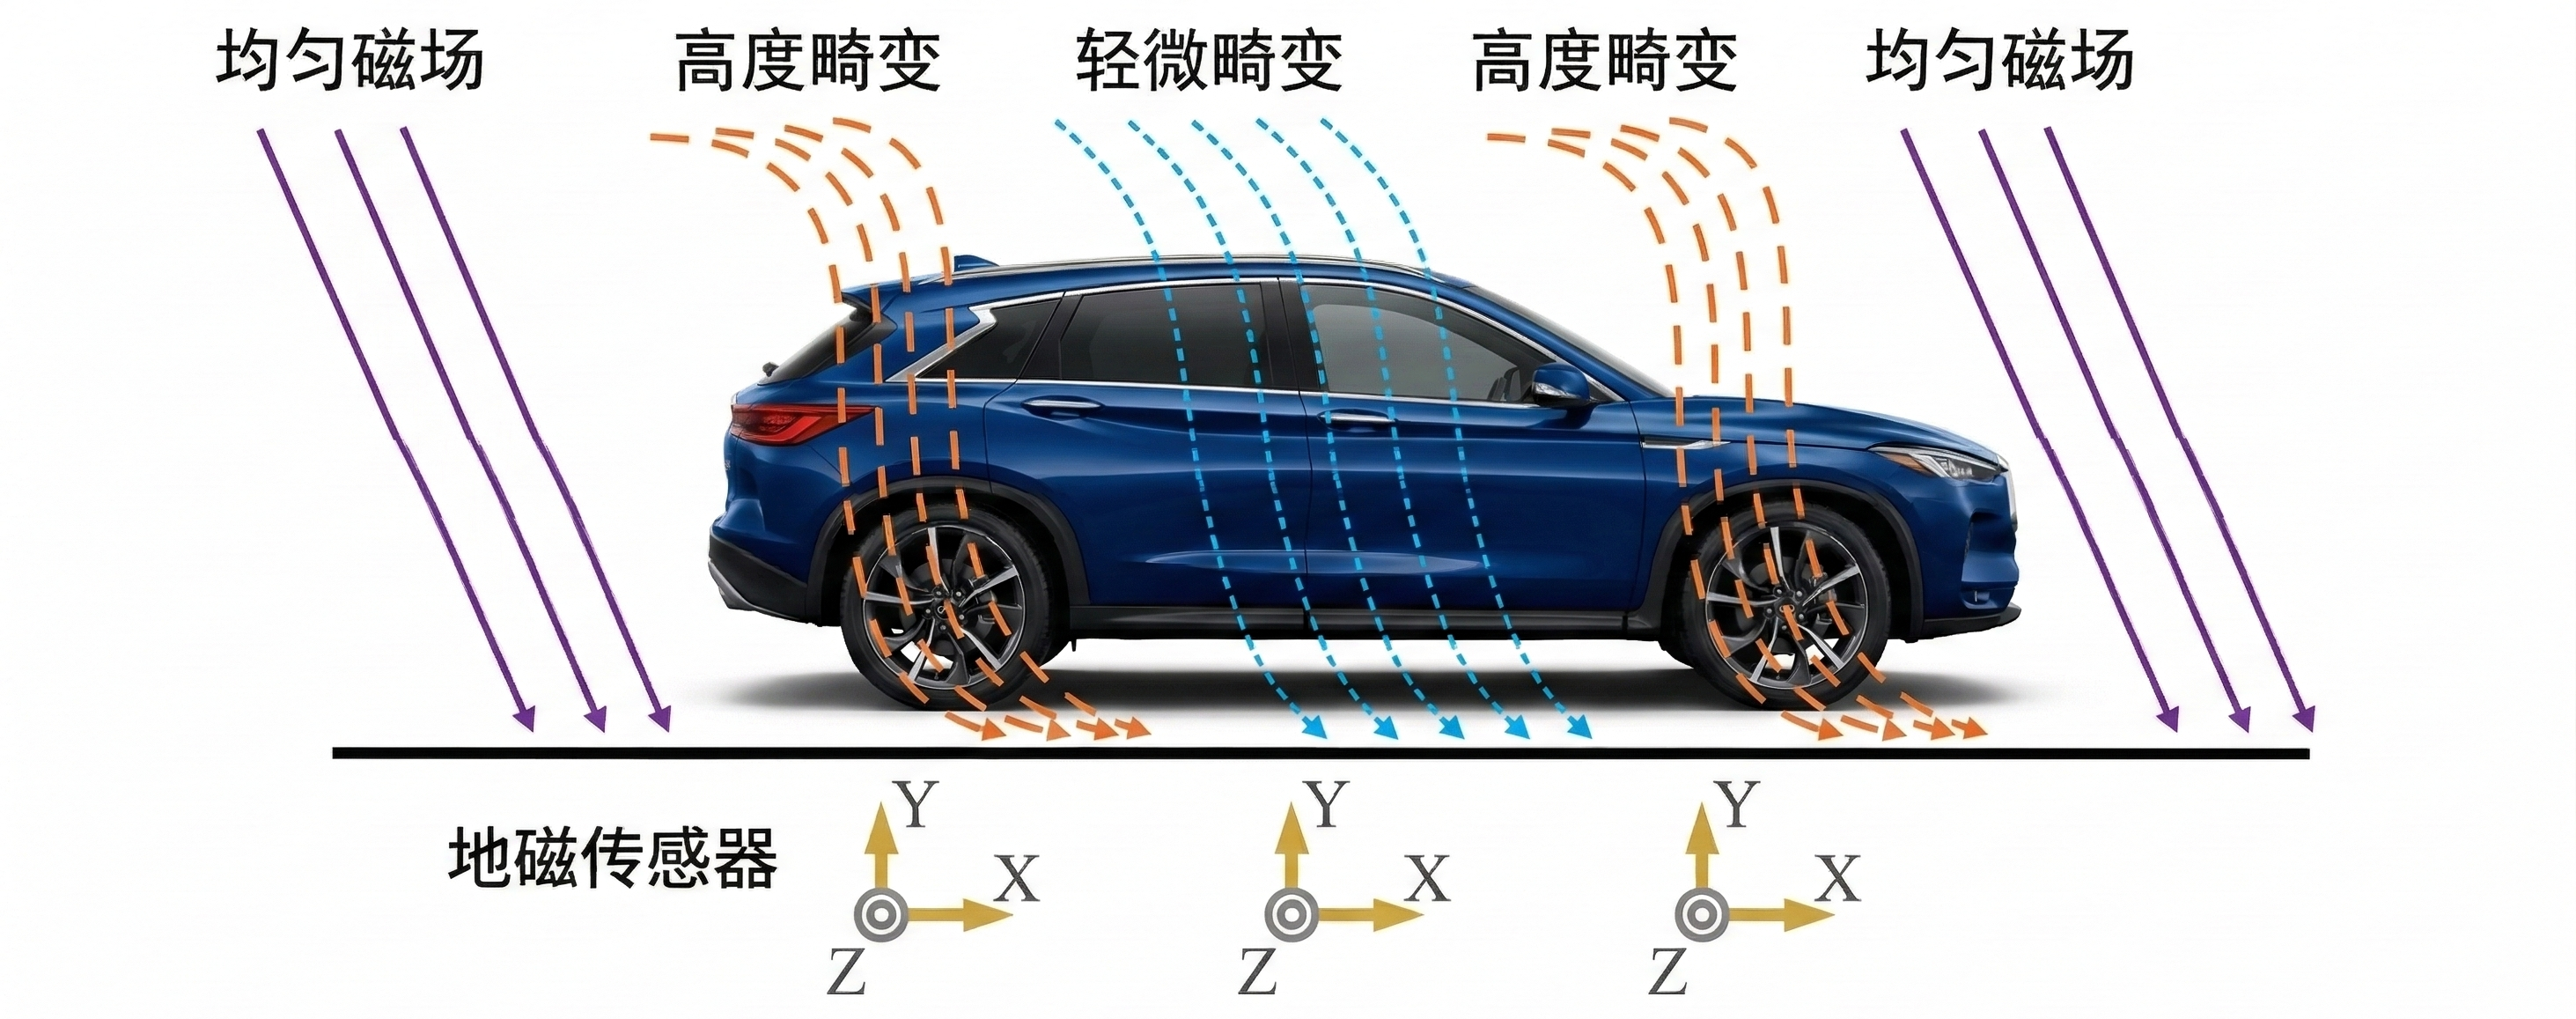
\includegraphics[width=0.85\textwidth]{images/chapter2/fig_2_1_mag_disturbance}
	\caption{车辆引起磁场扰动示意图}
	\label{fig:mag_disturbance}
\end{figure}

在上述机理基础上，地磁传感器可依据磁场相对基线的变化识别车辆进入和离开其有效作用范围。如图~\ref{fig:mag_value}所示，车辆经过时，传感器输出的磁场强度会在无车基线附近出现一段明显扰动，并在车辆离开后逐步恢复稳定。基于这段扰动过程，可以进一步提取车辆触发时间、持续时长、磁场扰动峰值等检测信息；结合多地磁传感器观测，这些信息还可为车辆类型判别等上层处理提供基础输入。因此，检测边界的稳定性与特征提取的一致性会直接影响后续目标跟踪效果。

\begin{figure}[htbp]
	\centering
	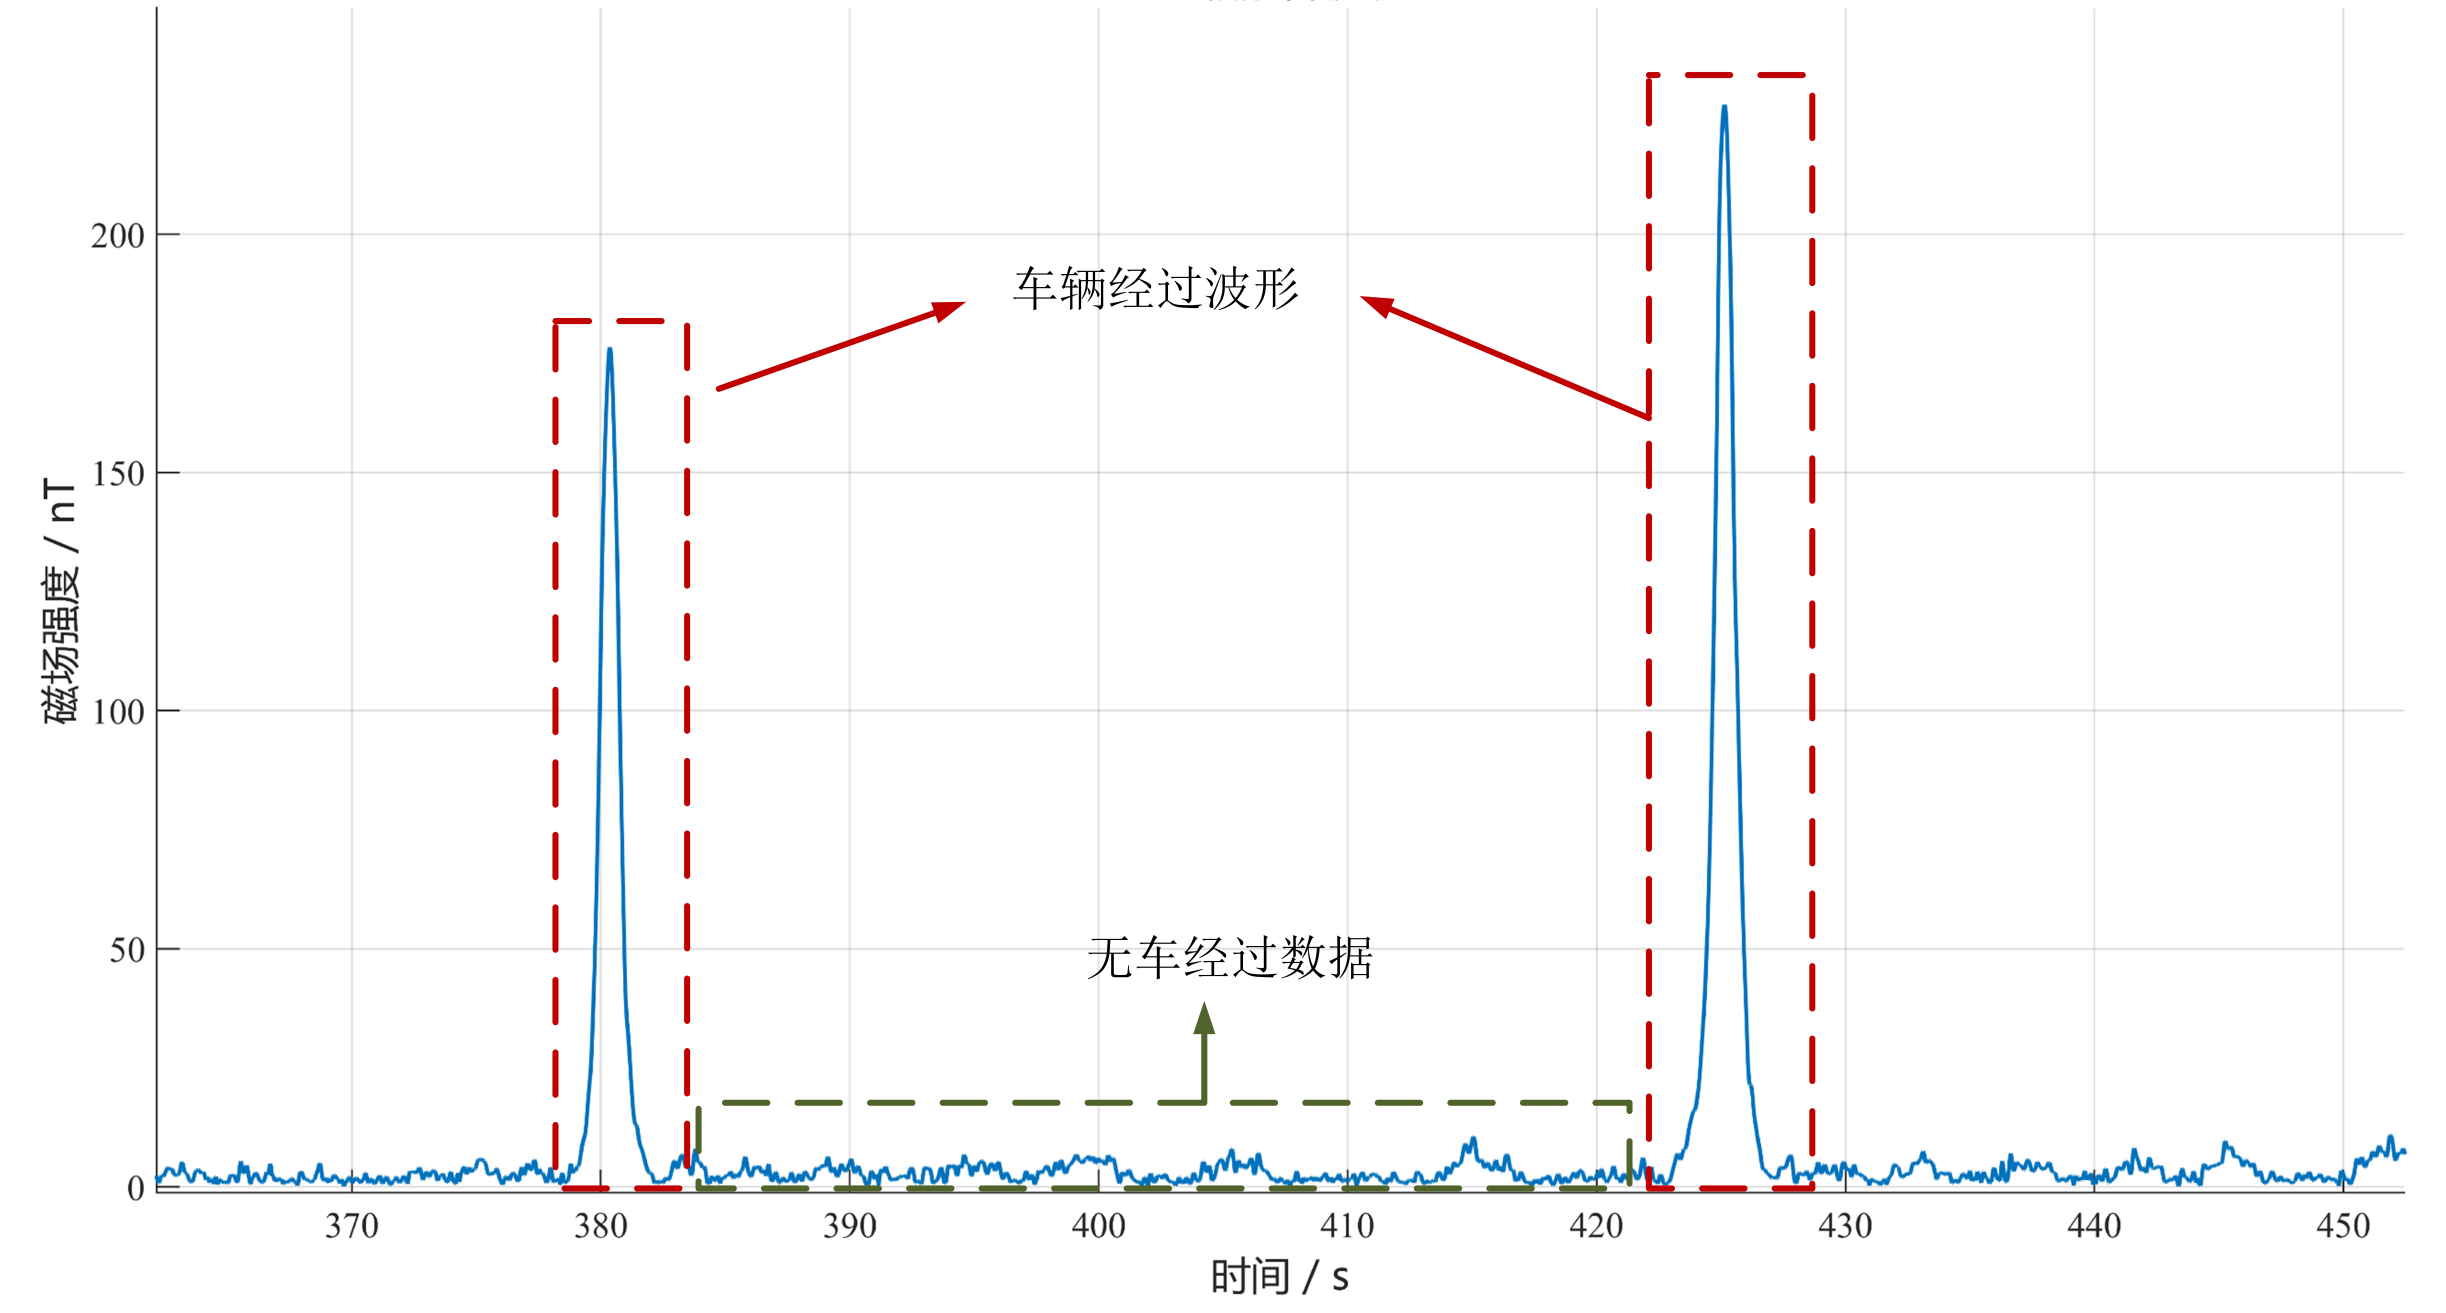
\includegraphics[width=0.85\textwidth]{images/chapter2/fig_2_2_mag_value}
	\caption{车辆经过时地磁传感器检测的磁场强度数据变化图}
	\label{fig:mag_value}
\end{figure}

同时需要注意，地磁扰动具有空间衰减特性。车辆与地磁传感器的横向距离增大时，传感器接收到的扰动幅值会下降，信噪比也随之降低；再叠加环境噪声、基线波动等因素影响，车辆通过时的磁场变化可能不再明显，从而出现漏检。

\subsection{地磁车辆检测算法}\label{sec:vehicle_detection}

地磁车辆检测的任务是在连续三轴磁场采样序列中识别由车辆通过引起的扰动区间，并在基线缓慢漂移与随机噪声叠加条件下保持触发稳定。不同系统在采样频率、特征构造和上报字段上存在差异，但基本处理流程较为一致：先对原始观测进行平滑去噪并在线估计无车基线，再将三轴相对基线的偏移量转换为标量检测统计量，最后通过阈值或状态机判决确定车辆是否进入和离开传感器有效作用范围，并据此生成检测数据\cite{ding2004signalprocessing,sarcevic2022singlemagnetometer}。

为便于统一判决，设传感器在第 $q$ 个采样时刻的三轴磁场观测向量和对应的标量检测统计量分别为
\begin{equation}
	\mathbf{B}(q)=
	\begin{bmatrix}
		B_x(q)\\
		B_y(q)\\
		B_z(q)
	\end{bmatrix}
	\label{eq:ch2_mag_observation_vector}
\end{equation}
\begin{equation}
	d(q)=\left\lVert \mathbf{B}(q)-\bar{\mathbf{B}}(q)\right\rVert_2
	\label{eq:ch2_mag_detection_scalar}
\end{equation}
其中，$B_x(q)$、$B_y(q)$、$B_z(q)$ 分别表示 $x$、$y$、$z$ 三个轴向的磁场分量观测值；$\bar{\mathbf{B}}(q)$ 表示对应时刻的无车基线估计向量，通常由滑动平均、低通滤波或递推估计获得。式~\eqref{eq:ch2_mag_detection_scalar}实质上是将三个轴向相对基线的偏移量融合为一个标量，用于表征当前采样时刻整体磁场扰动强度。这样，无论扰动主要体现在哪个轴向上，都可以在同一尺度下进行比较和阈值判决。由于 $d(q)$ 会随车型、车速、车辆相对传感器的通过位置以及姿态等因素产生幅值波动，同时基线也可能随温度或环境磁背景变化而缓慢漂移，因此检测阶段通常需要采用阈值自适应或引入序列一致性约束，以降低长期部署中阈值失配与抖动触发带来的稳定性下降\cite{sarcevic2022singlemagnetometer}。

在判决逻辑上，阈值判决通过比较 $d(q)$ 与阈值 $T$ 实现二值判定：当 $d(q)>T$ 时判为有车，否则判为无车，其中 $T$ 为判决阈值。该方法结构简单、计算代价低，适合在传感器端实时运行，但固定阈值对幅值变化与基线漂移较为敏感。为提升不同工况下的可用性，可采用自适应阈值策略，根据近期噪声水平或统计量分布对 $T$ 进行在线更新，从而在车辆幅值变化或背景波动时维持较稳定的检出性能。

仅依赖逐点阈值比较时，$d(q)$ 在阈值附近的波动可能引发重复触发或短脉冲误检。为减小这类影响，工程实现中常在阈值判决基础上引入有限状态机（Finite State Machine, FSM）判决机制。如图~\ref{fig:ch2_fsm_detection}所示，FSM 可将检测过程划分为无车、进入确认、有车和离开确认四个状态，并结合连续点数或最小持续时间约束完成状态转移：当进入条件连续满足一定长度时，确认车辆进入；当离开条件连续满足一定长度时，确认车辆离开。这样可以避免统计量在阈值附近短时波动时频繁切换状态，从而提高对噪声和突发干扰的容忍度。在多车道场景下，还可进一步结合多轴一致性、滞回阈值或车道约束等机制，降低相邻车道干扰引发的误检概率\cite{guilbert2016statemachine}。

\begin{figure}[htbp]
	\centering
	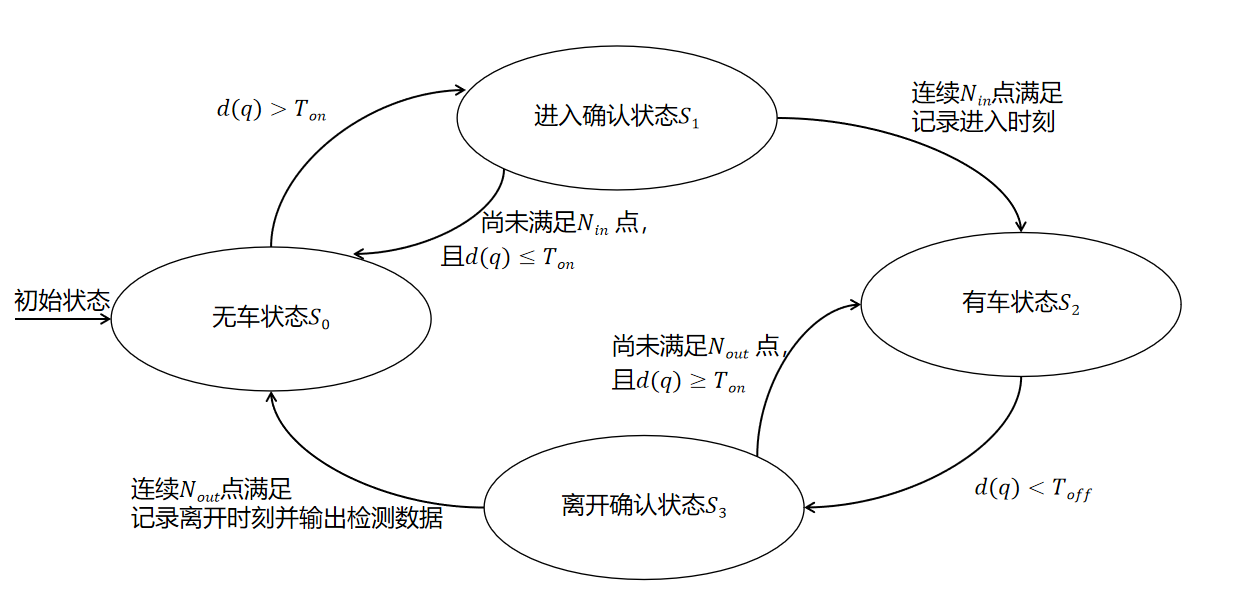
\includegraphics[width=0.82\textwidth]{images/chapter2/fig_2_3_fsm_detection}
	\caption{FSM状态机判决示意图}
	\label{fig:ch2_fsm_detection}
\end{figure}

当进入时刻和离开时刻被稳定确定后，系统即可生成一条车辆检测数据。该数据通常以进入时刻和离开时刻表征车辆在地磁传感器有效探测区内的通过区间，并可进一步输出扰动峰值、持续时长等特征字段，为速度估计、占有率计算、车长推断以及跨点数据关联提供基础量测输入\cite{balid2018intelligent}。


\section{卡尔曼滤波算法}

由于存在杂波干扰以及传感器测量误差，传感器输出与目标真实状态之间通常会有偏差，因此需要借助滤波算法对目标状态进行估计，以减弱不确定性带来的影响。卡尔曼滤波是多目标跟踪中常用的滤波方法之一，主要适用于线性动态系统。其基本思想是先依据目标运动模型对下一时刻状态进行预测，再将预测结果与传感器测量进行加权融合，从而得到目标运动状态的估计。该方法只需保留前一时刻的状态估计结果，计算复杂度相对较低，并且在线性系统中具有较好的跟踪性能。

\subsection{卡尔曼滤波算法的过程}

在卡尔曼滤波中，首先需要建立目标运动模型与观测模型，其离散时间状态方程分别为
\begin{equation}
	x(k)=F(k-1)x(k-1)+W(k-1)
\end{equation}

\begin{equation}
	z(k)=H(k)x(k)+V(k)
\end{equation}

其中，$x(k)$ 表示 $k$ 时刻目标的运动状态，$F(k-1)$ 为目标的状态转移矩阵；$z(k)$ 表示 $k$ 时刻的测量，$H(k)$ 为系统的观测矩阵。$W(k-1)$ 为系统的过程噪声，$V(k)$ 为系统的测量噪声。假设过程噪声与测量噪声相互独立，且都服从均值为零的高斯分布，则有
\begin{equation}
	E\!\left(W(k)W^{T}(j)\right)=Q(k)\delta_{kj}
\end{equation}

\begin{equation}
	E\!\left(V(k)V^{T}(j)\right)=R(k)\delta_{kj}
\end{equation}

\begin{equation}
	E\!\left(W(k)V^{T}(k)\right)=0
\end{equation}

其中，$Q(k)$ 为 $k$ 时刻系统过程噪声的协方差矩阵，$R(k)$ 为 $k$ 时刻系统测量噪声的协方差矩阵。$\delta_{kj}$ 为 Delta 函数，其定义为
\begin{equation}
	\delta_{kj}=
	\begin{cases}
		1, & k=j,\\
		0, & k\neq j.
	\end{cases}
\end{equation}

卡尔曼滤波的估计过程包括状态预测和测量更新两个步骤。状态预测利用当前时刻的状态估计对下一时刻的目标状态进行预测，其计算公式为
\begin{equation}
	\hat{x}(k|k-1)=F(k-1)\hat{x}(k-1|k-1)
\end{equation}

\begin{equation}
	P(k|k-1)=F(k-1)P(k-1|k-1)F^{T}(k-1)+Q(k-1)
\end{equation}

其中，$\hat{x}(k|k-1)$ 表示利用 $k-1$ 时刻信息得到的 $k$ 时刻目标状态预测，$P(k|k-1)$ 为对应的预测协方差矩阵。

测量更新用于融合测量信息与状态预测，以得到更优的后验估计。首先计算新息向量
\begin{equation}
	\nu(k)=z(k)-H(k)\hat{x}(k|k-1)
\end{equation}

新息的协方差矩阵为
\begin{equation}
	S(k)=H(k)P(k|k-1)H^{T}(k)+R(k)
\end{equation}

卡尔曼滤波增益为
\begin{equation}
	K(k)=P(k|k-1)H^{T}(k)S^{-1}(k)
\end{equation}

最终的滤波结果为
\begin{equation}
	\hat{x}(k|k)=\hat{x}(k|k-1)+K(k)\nu(k)
\end{equation}

\begin{equation}
	P(k|k)=P(k|k-1)-K(k)H(k)P(k|k-1)
\end{equation}

其中，$\hat{x}(k|k)$ 为 $k$ 时刻目标运动状态的后验估计，$P(k|k)$ 为对应的状态估计协方差矩阵。

卡尔曼滤波器的性能在很大程度上取决于目标运动模型的选取。下面介绍卡尔曼滤波器中常见的运动模型及其过程噪声的选取。

\subsection{目标运动模型}

卡尔曼滤波以及大多数跟踪器都建立在目标运动模型的基础上。目标运动模型描述了目标运动状态随时间的变化规律，选择合适的目标运动模型有助于提高目标状态估计的准确性。根据目标的运动学特征，常见的目标运动模型包括常速度（Constant Velocity，CV）模型、常加速度（Constant Acceleration，CA）模型以及匀速转弯（Constant Turn，CT）模型等。

\textnormal{（1）CA 模型}\par\vspace{0.3\baselineskip}

常速度模型假设目标做匀速直线运动。在理想情况下，目标加速度应为零；但在实际应用中，受外界干扰影响，加速度通常不可能严格为零。因此，CV 模型将加速度视为均值为零的高斯白噪声，用来描述这部分扰动。

状态转移矩阵为
\begin{equation}
	F(k)=
	\begin{bmatrix}
		1 & T_k\\
		0 & 1
	\end{bmatrix}
\end{equation}

噪声增益向量为
\begin{equation}
	\Gamma(k)=
	\begin{bmatrix}
		\dfrac{1}{2}T_k^2\\
		T_k
	\end{bmatrix}
\end{equation}

过程噪声的协方差矩阵为
\begin{equation}
	Q(k)=\Gamma(k)\sigma_w^2\Gamma^{T}(k)=
	\begin{bmatrix}
		\dfrac{1}{4}T_k^4 & \dfrac{1}{2}T_k^3\\[6pt]
		\dfrac{1}{2}T_k^3 & T_k^2
	\end{bmatrix}\sigma_w^2
\end{equation}

其中，$T_k$ 为 $k-1$ 时刻与 $k$ 时刻之间的时间间隔，$\sigma_w$ 表示过程噪声的标准差。文献[19]指出，CV 模型中 $\sigma_w$ 的取值与目标最大加速度 $a_M$ 的数量级有关，在实际使用中可取
\[
0.5a_M \leq \sigma_w \leq a_M.
\]

\textnormal{（2）CA 模型}\par\vspace{0.3\baselineskip}

常加速度模型假设过程噪声 $W(k)$ 为加速度的增量，该增量是均值为零的白噪声序列，也就是说，加速度满足离散时间维纳过程。以目标在一维空间中的运动为例，其状态向量由位置、速度和加速度组成。

状态转移矩阵为
\begin{equation}
	F(k)=
	\begin{bmatrix}
		1 & T_k & \dfrac{T_k^2}{2}\\
		0 & 1   & T_k\\
		0 & 0   & 1
	\end{bmatrix}
\end{equation}

噪声增益向量为
\begin{equation}
	\Gamma(k)=
	\begin{bmatrix}
		\dfrac{T_k^2}{2}\\
		T_k\\
		1
	\end{bmatrix}
\end{equation}

过程噪声的协方差矩阵为
\begin{equation}
	Q(k)=\Gamma(k)\sigma_q^2\Gamma^{T}(k)=
	\begin{bmatrix}
		\dfrac{1}{4}T_k^4 & \dfrac{1}{2}T_k^3 & \dfrac{1}{2}T_k^2\\[6pt]
		\dfrac{1}{2}T_k^3 & T_k^2 & T_k\\[6pt]
		\dfrac{1}{2}T_k^2 & T_k & 1
	\end{bmatrix}\sigma_q^2
\end{equation}

文献[19]关于 CA 模型的讨论表明，$\sigma_q$ 的取值与两次更新时刻之间目标的最大加速度增量 $\Delta a_M$ 有关，在实际使用中可取
\[
0.5\Delta a_M \leq \sigma_q \leq \Delta a_M.
\]

\textnormal{（3）CT 模型}\par\vspace{0.3\baselineskip}

CT 模型主要用于描述目标运动过程中的转弯状态。该模型假设目标在转弯时保持匀角速度运动，并通过设置转弯角速度对目标转弯过程中的状态进行估计。令 $\omega$ 表示目标的转弯角速度，在二维坐标系中，目标的状态向量为
\[
x(k)=[x,\ v_x,\ y,\ v_y]^T,
\]
则 CT 模型的离散状态方程为
\begin{equation}
	x(k+1)=
	\begin{bmatrix}
		1 & \dfrac{\sin \omega T}{\omega} & 0 & -\dfrac{1-\cos \omega T}{\omega}\\[8pt]
		0 & \cos \omega T & 0 & -\sin \omega T\\[6pt]
		0 & \dfrac{1-\cos \omega T}{\omega} & 1 & \dfrac{\sin \omega T}{\omega}\\[8pt]
		0 & \sin \omega T & 0 & \cos \omega T
	\end{bmatrix}
	x(k)
	+
	\begin{bmatrix}
		\dfrac{T^2}{2}\\
		T\\
		\dfrac{T^2}{2}\\
		T
	\end{bmatrix}
	w(k)
\end{equation}

其中，$T$ 为相邻时刻之间的时间间隔，$w(k)$ 为过程噪声。目标转弯角速度 $\omega$ 决定了目标的转弯速度和转弯方向，因此 CT 模型能够用于描述正在转弯的机动目标。


\section{数据关联算法}\label{sec:orm}

在多目标跟踪中，滤波器可以根据历史信息给出每条轨迹在下一时刻的预测状态，但当前到来的量测并不自带“目标身份”，因此还需要判断每个量测应由哪条轨迹吸收更新，这一步就是数据关联。若关联错误，错误量测会直接进入状态更新，进而造成轨迹漂移、身份切换甚至轨迹中断。因此，数据关联的核心任务不是简单地“找最近的量测”，而是在漏检、杂波和目标并行运动同时存在的情况下，为每条轨迹选择最合理的更新对象。考虑到本文后续主要用到跟踪波门、确定性分配、概率关联和多扫描一致性四类思想，本节只围绕这几部分进行说明。

设更新时刻为 $t_k$，当前共有 $N_k$ 条待更新轨迹，接收到的量测集合记为
\begin{equation}
	\mathcal{Z}_k=
	\left\{
	\mathbf{z}^{(1)}_k,\mathbf{z}^{(2)}_k,\ldots,\mathbf{z}^{(M_k)}_k
	\right\},
\end{equation}
其中，$M_k$ 表示当前时刻的量测数，$\mathbf{z}^{(j)}_k$ 表示第 $j$ 个量测。对第 $i$ 条轨迹，滤波器已经给出预测状态 $\hat{\mathbf{x}}^{(i)}_{k|k-1}$ 和预测协方差 $\mathbf{P}^{(i)}_{k|k-1}$。数据关联要解决的问题，就是判断 $\mathcal{Z}_k$ 中哪些量测可以用于更新第 $i$ 条轨迹，哪些量测应视为杂波或新目标候选；若某条轨迹在 $t_k$ 没有找到合适量测，则对应一次漏检。

\subsection{跟踪波门}

数据关联通常不会一开始就对全部轨迹和全部量测逐一比较，而是先排除明显不可能的轨迹--量测组合。这个预筛选区域称为跟踪波门。波门的作用有两个：一是减少后续关联计算量，二是尽量把不合理匹配挡在关联阶段之外。

在第2.4节给出的线性观测模型下，轨迹 $i$ 在时刻 $t_k$ 的预测量测为
\begin{equation}
	\hat{\mathbf{z}}^{(i)}_{k|k-1}=\mathbf{H}_k\hat{\mathbf{x}}^{(i)}_{k|k-1},
\end{equation}
其中，$\mathbf{H}_k$ 为量测矩阵。若将第 $j$ 个量测与轨迹 $i$ 进行比较，则对应的创新向量为
\begin{equation}
	\boldsymbol{\nu}^{(i,j)}_k
	=
	\mathbf{z}^{(j)}_k-\hat{\mathbf{z}}^{(i)}_{k|k-1}.
\end{equation}
创新协方差为
\begin{equation}
	\mathbf{S}^{(i)}_k
	=
	\mathbf{H}_k\mathbf{P}^{(i)}_{k|k-1}\mathbf{H}_k^{\top}+\mathbf{R}_k,
\end{equation}
其中，$\mathbf{R}_k$ 为量测噪声协方差矩阵。进一步定义轨迹 $i$ 与量测 $j$ 之间的平方马氏距离为
\begin{equation}
	d_k^2(i,j)
	=
	\left(\boldsymbol{\nu}^{(i,j)}_k\right)^{\top}
	\left(\mathbf{S}^{(i)}_k\right)^{-1}
	\boldsymbol{\nu}^{(i,j)}_k.
\end{equation}
给定波门阈值 $\gamma$ 后，轨迹 $i$ 的椭球波门可写为
\begin{equation}
	\mathcal{G}^{(i)}_k
	=
	\left\{
	j\,\big|\, d_k^2(i,j)\le \gamma
	\right\}.
\end{equation}
式中，$\mathcal{G}^{(i)}_k$ 表示落入轨迹 $i$ 波门内的量测编号集合。若量测维数为 $m$，常将阈值取为 $\gamma=\chi_m^2(P_G)$，其中，$\chi_m^2(\cdot)$ 表示自由度为 $m$ 的卡方分布分位函数，$P_G$ 为真实量测被波门保留的概率。这样一来，只有满足 $d_k^2(i,j)\le \gamma$ 的量测才会进入后续关联计算。其直观含义是：当轨迹预测更准确、协方差更小时，波门会更紧；当不确定性增大时，波门会相应放宽。

\subsection{硬关联方法}

当波门内的候选关系比较清晰时，可以直接给出唯一的一对一分配结果，这类方法称为硬关联。它的基本思想是在当前时刻，从所有候选轨迹--量测对中选出一组总代价最小且互不冲突的匹配关系。

定义二值分配变量
\begin{equation}
	a_{i,j}=
	\begin{cases}
		1, & \text{量测 } \mathbf{z}^{(j)}_k \text{分配给轨迹 } i,\\
		0, & \text{否则}.
	\end{cases}
\end{equation}
若记 $c_{i,j}$ 为量测 $j$ 分配给轨迹 $i$ 的代价，则单时刻的一对一分配问题可写为
\begin{align}
	\min_{\{a_{i,j}\}}\quad
	& \sum_{i=1}^{N_k}\sum_{j=1}^{M_k} c_{i,j}a_{i,j} \\
	\text{s.t.}\quad
	& a_{i,j}\in\{0,1\}, \\
	& \sum_{j=1}^{M_k} a_{i,j}\le 1,\qquad i=1,2,\ldots,N_k, \\
	& \sum_{i=1}^{N_k} a_{i,j}\le 1,\qquad j=1,2,\ldots,M_k.
\end{align}
其中，$c_{i,j}$ 可以取平方马氏距离，也可以取负对数似然；第一个约束表示每条轨迹至多分配一个量测，第二个约束表示每个量测至多分配给一条轨迹。若某个轨迹--量测对不在波门内，通常将其代价设为一个很大的惩罚值，从而避免不合理匹配被选中。该类线性指派问题可用匈牙利算法高效求解\cite{kuhn1955hungarian}。硬关联方法实现简单、计算量较低，但在量测拥挤或目标间距离很近时，一旦分配错误，误关联会直接传递到状态更新阶段。

\subsection{概率数据关联方法}

当一条轨迹的波门内同时出现多个都“看起来合理”的候选量测时，强行做唯一分配往往不够稳健。概率数据关联方法不急于只选一个量测，而是先为各候选量测计算关联概率，再按概率进行加权更新。PDA 主要针对单轨迹场景，JPDA 则进一步考虑多轨迹之间的量测互斥关系\cite{barshalom1975pda,fortmann1983jpda}。


\textnormal{(1) PDA的基本形式}\par\vspace{0.3\baselineskip}

对于轨迹 $i$，若量测 $j\in\mathcal{G}^{(i)}_k$ 落入其波门内，则该量测的似然可写为
\begin{equation}
	L_{i,j}
	=
	\mathcal{N}\!\left(
	\mathbf{z}^{(j)}_k;
	\hat{\mathbf{z}}^{(i)}_{k|k-1},
	\mathbf{S}^{(i)}_k
	\right),
\end{equation}
其中，$L_{i,j}$ 表示量测 $j$ 由轨迹 $i$ 生成的似然值，$\mathcal{N}(\cdot;\boldsymbol{\mu},\mathbf{\Sigma})$ 表示均值为 $\boldsymbol{\mu}$、协方差为 $\mathbf{\Sigma}$ 的高斯概率密度函数。考虑漏检和杂波后，PDA 中常用的关联概率写为
\begin{equation}
	\beta_{i,j}
	=
	\frac{P_D L_{i,j}}
	{\lambda_c V_k^{(i)}+P_D\sum\limits_{\ell\in\mathcal{G}^{(i)}_k}L_{i,\ell}},
\end{equation}
对应的漏检概率为
\begin{equation}
	\beta_{i,0}
	=
	1-\sum_{j\in\mathcal{G}^{(i)}_k}\beta_{i,j}.
\end{equation}
式中，$P_D$ 为检测概率，$\lambda_c$ 为杂波空间密度，$V_k^{(i)}$ 为轨迹 $i$ 在时刻 $t_k$ 的波门体积，$\beta_{i,j}$ 表示量测 $j$ 与轨迹 $i$ 的关联概率，$\beta_{i,0}$ 表示轨迹 $i$ 在当前时刻漏检的概率。

得到关联概率后，可先构造加权创新
\begin{equation}
	\bar{\boldsymbol{\nu}}^{(i)}_k
	=
	\sum_{j\in\mathcal{G}^{(i)}_k}
	\beta_{i,j}\boldsymbol{\nu}^{(i,j)}_k,
\end{equation}
再按加权创新完成状态更新：
\begin{equation}
	\hat{\mathbf{x}}^{(i)}_{k|k}
	=
	\hat{\mathbf{x}}^{(i)}_{k|k-1}
	+
	\mathbf{K}^{(i)}_k\bar{\boldsymbol{\nu}}^{(i)}_k,
\end{equation}
其中，$\mathbf{K}^{(i)}_k$ 为第 $i$ 条轨迹的卡尔曼增益，其形式与第2.4节一致。上式说明，PDA 并不只使用单个量测更新轨迹，而是让所有候选量测按各自概率共同参与更新。这样做虽然会使更新更加“保守”，但在候选量测彼此接近时通常比硬关联更稳健。实际实现中，协方差更新还会额外考虑关联不确定性带来的膨胀效应，以避免在歧义较强时对状态估计过度自信。


\textnormal{(2) JPDA的基本形式}\par\vspace{0.3\baselineskip}

如果场景中同时存在多条轨迹，且它们共用同一批门内量测，仅对每条轨迹独立使用 PDA 会忽略量测互斥关系。例如，同一个量测可能被两条轨迹同时赋予较高权重。JPDA 的基本思路是：先从整体上考虑“所有轨迹与所有量测如何同时匹配”，再把联合假设的概率分摊回单条轨迹。

定义联合关联变量向量为
\begin{equation}
	\boldsymbol{\theta}_k
	=
	\left[
	\theta_k^{(1)},\theta_k^{(2)},\ldots,\theta_k^{(N_k)}
	\right]^{\top},
\end{equation}
其中，$\theta_k^{(i)}=j$ 表示轨迹 $i$ 与量测 $j$ 关联，$\theta_k^{(i)}=0$ 表示轨迹 $i$ 在当前时刻漏检。设 $\Theta_k$ 为所有满足一对一约束的可行联合假设集合，则轨迹 $i$ 与量测 $j$ 的边缘关联概率为
\begin{equation}
	\beta_{i,j}
	=
	\sum_{\boldsymbol{\theta}_k\in\Theta_k:\,\theta_k^{(i)}=j}
	p(\boldsymbol{\theta}_k\mid \mathcal{Z}_k),
\end{equation}
对应的漏检概率为
\begin{equation}
	\beta_{i,0}
	=
	\sum_{\boldsymbol{\theta}_k\in\Theta_k:\,\theta_k^{(i)}=0}
	p(\boldsymbol{\theta}_k\mid \mathcal{Z}_k).
\end{equation}
式中，$p(\boldsymbol{\theta}_k\mid \mathcal{Z}_k)$ 表示联合假设 $\boldsymbol{\theta}_k$ 在当前量测集合 $\mathcal{Z}_k$ 下的后验概率。得到 $\beta_{i,j}$ 后，各条轨迹仍可按 PDA 的方式完成加权更新。与 PDA 相比，JPDA 显式考虑了“一个量测不能同时分配给多条轨迹”的约束，因此在多目标近距离同行、交汇或短时并行场景中通常更加稳定；但其代价是联合假设数量会随着轨迹数和量测数迅速增加，计算量明显上升。

\subsection{多扫描关联与一致性推断}

前述方法大多在单个更新时刻内完成关联判断，优点是响应快，但缺点是容易受到瞬时噪声、短时漏检以及目标近距离并行的影响。多扫描关联的思路是，不只利用当前时刻的量测，而是在一个有限时间窗口内综合多帧信息，从而利用目标运动的时间连续性来提高关联稳定性\cite{reid1979mht}。

设固定滞后窗口长度为 $L$，则窗口内的量测序列可记为
\begin{equation}
	\mathcal{Z}_{k-L+1:k}
	=
	\left\{
	\mathcal{Z}_{k-L+1},\mathcal{Z}_{k-L+2},\ldots,\mathcal{Z}_k
	\right\},
\end{equation}
对应的关联决策序列记为
\begin{equation}
	\boldsymbol{\theta}_{k-L+1:k}
	=
	\left\{
	\boldsymbol{\theta}_{k-L+1},\boldsymbol{\theta}_{k-L+2},\ldots,\boldsymbol{\theta}_k
	\right\}.
\end{equation}
在该窗口内，可将关联问题写为最大后验估计形式：
\begin{equation}
	\hat{\boldsymbol{\theta}}_{k-L+1:k}
	=
	\arg\max_{\boldsymbol{\theta}_{k-L+1:k}}
	p\!\left(
	\boldsymbol{\theta}_{k-L+1:k}
	\mid
	\mathcal{Z}_{k-L+1:k}
	\right).
\end{equation}
式中，$L$ 表示窗口长度，$\mathcal{Z}_{k-L+1:k}$ 表示窗口内全部量测，$\boldsymbol{\theta}_{k-L+1:k}$ 表示对应的关联决策序列，$\hat{\boldsymbol{\theta}}_{k-L+1:k}$ 表示后验概率最大的关联结果。这个式子的含义可以直接理解为：系统并不是只寻找“当前这一帧最像谁”的匹配，而是在一段连续时间内寻找“整体最连贯”的关联序列。窗口越长，可利用的时间信息越充分，关联结果通常越稳定；但与此同时，计算量和输出滞后也会增加。因此，工程实现中常采用固定滞后窗口、假设剪枝和局部回放等方式，在实时性与稳定性之间进行折中。

综上，数据关联的基本思路可以概括为：先利用跟踪波门缩小候选范围，再根据场景复杂度选择硬关联或概率关联，并在必要时引入多扫描信息提高跨时刻一致性。本文后续章节将在这些基础思想之上，结合地磁事件流异步到达的特点，对门控方式、关联代价和固定滞后处理流程做进一步设计。


\section{实时聚类算法}

\subsection{数据流基本概念}

本文中，多地磁传感器系统上传到后台的检测记录会随时间持续到达，因此在处理方式上本质上属于数据流。与一次性给出的静态数据集不同，数据流并不会在算法开始前完整可见，而是随着系统运行不断生成并进入处理链路。上一节用 $\mathbf z_j$ 表示按到达顺序接收的第 $j$ 条原始量测，强调的是地磁量测的物理含义；本节为了讨论聚类算法的一般形式，将进入聚类模块的第 $j$ 个样本统一记为 $\mathbf x_j$。当聚类输入直接由原始量测构成时，$\mathbf x_j$ 可以看作 $\mathbf z_j$ 的抽象表示；若在进入聚类前还进行了特征构造、样本重组或状态融合，则 $\mathbf x_j$ 表示相应处理后的聚类样本。于是，数据流可表示为
\begin{equation}
	\mathcal{X}=\left\{\mathbf{x}_j\right\}_{j=1}^{\infty},
\end{equation}
其中 $\mathbf{x}_j\in\mathbb{R}^d$ 表示第 $j$ 个到达的 $d$ 维样本。

数据流处理的首要特点，是算法通常只能按照样本的到达次序进行一次性访问。由于样本会持续生成，数据规模也会不断增长，系统往往无法像离线方法那样反复遍历全部历史数据，也难以长期保存完整原始样本。对于交通感知、工业监测和网络业务等在线场景而言，系统还需要在新样本到达后较短时间内完成判断与更新，因此计算复杂度、存储开销和响应延迟都会直接影响算法能否稳定运行。

另一个重要特点是数据分布可能随时间变化。随着交通状态、环境噪声以及设备工作状态的改变，早期样本所反映的分布未必仍能代表当前状态。如果聚类结果长期受旧样本主导，算法对最新模式的响应能力就会下降。为此，数据流聚类通常会引入时间敏感机制，例如仅保留最近一段样本的滑动窗口，或通过衰减因子逐步降低旧样本的影响，使簇结构能够更及时地反映当前数据分布。

因此，数据流聚类关注的重点，不是对一批固定样本做一次性划分，而是在样本持续到达的过程中对簇结构进行增量维护。算法既要判断新样本应归入哪个簇，也要处理新簇生成、簇状态更新、簇失活和簇删除等问题。这种面向持续更新的处理方式，是数据流聚类区别于传统离线聚类的关键所在。

\subsection{实时聚类算法}

数据流聚类算法的核心任务，是在样本持续到达的条件下维持可用的簇结构。按照聚类结果形成的时机不同，现有方法大致可以分为两类：一类在在线阶段维护数据摘要，并在需要时由离线阶段生成聚类结果；另一类在样本到达后直接完成归类与簇状态更新。前者更强调摘要压缩能力，后者更强调结果的实时可用性。下面分别进行说明。


\textnormal{(1) 两阶段流聚类算法}\par\vspace{0.3\baselineskip}

两阶段流聚类算法采用在线处理与离线分析相结合的框架，代表性方法是 CluStream\cite{aggarwal2003clustream}。这类方法在在线阶段持续接收数据流，并利用有限存储结构维护局部统计摘要；当系统需要输出聚类结果时，再由离线阶段基于这些摘要执行进一步的聚类分析。由于计算量较大的聚类运算被转移到离线阶段，因此在线链路的实时处理压力可以得到明显缓解。

\begin{figure}[htbp]
	\centering
	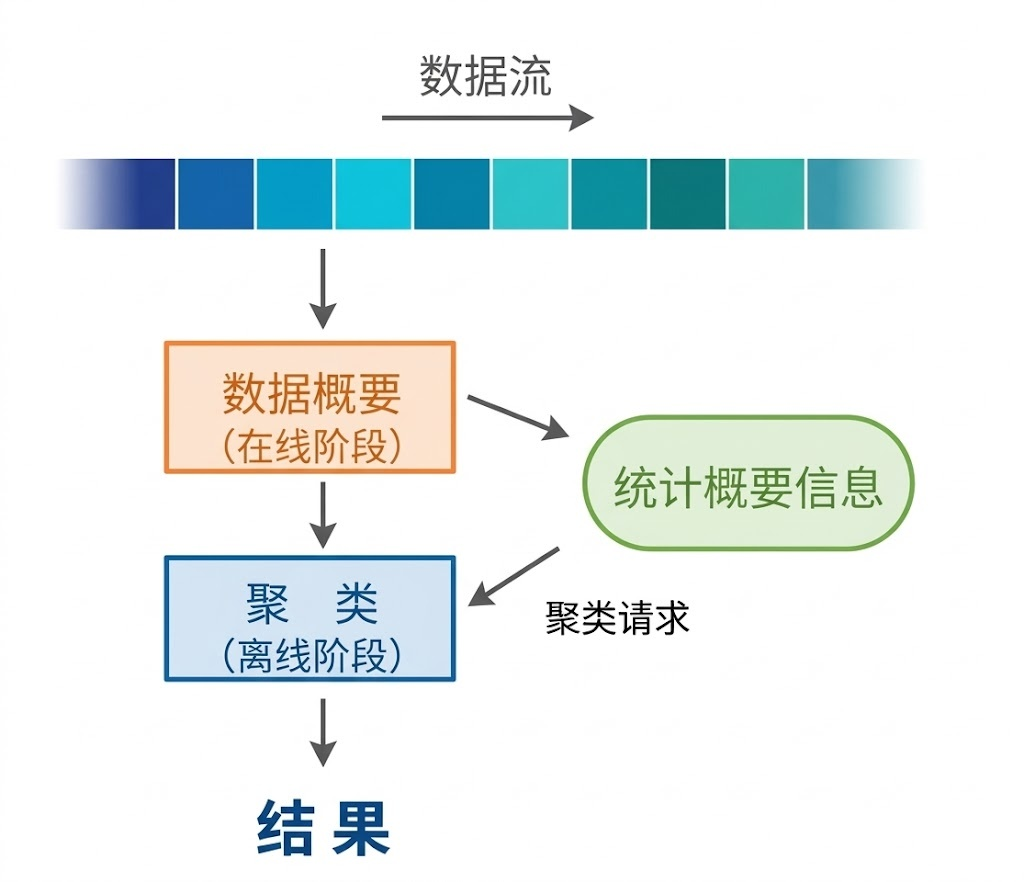
\includegraphics[width=0.65\textwidth]{images/chapter2/two_stage}
	\caption{两阶段流聚类处理框架图}
	\label{two_stage}
\end{figure}

这类方法的关键在于微簇。微簇并不保存全部历史样本，而是用簇中心、样本数以及离散程度等统计量对局部数据分布进行紧凑表示。当新样本到达时，算法首先判断其是否可以并入某个已有微簇；若可以并入，则更新该微簇的统计摘要；若不能归入现有微簇，则根据当前资源约束创建新的微簇，或对旧的摘要结构进行替换和压缩。由于在线阶段只需维护数量有限的微簇，因此这类方法在大规模数据流场景中通常具有较好的可扩展性。

离线阶段则以微簇摘要为输入，进一步形成宏观聚类结果。以 CluStream 为例，在线阶段持续维护微簇，离线阶段可在用户指定的时间范围内对这些微簇执行 $k$-means 等宏聚类操作，从而得到最终聚类结果。在 CluStream 之后，DenStream\cite{cao2006denstream} 又进一步引入潜在微簇、离群微簇以及衰减机制，以增强两阶段框架对噪声和分布变化的适应能力。总体来看，两阶段方法的优势在于在线阶段负担较轻，适合以摘要维护为主的大规模数据流场景；其不足则在于最终结果仍依赖额外的离线处理，因此当系统需要持续输出当前聚类结果时，使用上会受到一定限制。

\textnormal{(2) 完全在线聚类算法}\par\vspace{0.3\baselineskip}

完全在线聚类算法不再把聚类结果的形成推迟到离线阶段，而是要求系统在新样本到达后立即做出归类决策，并同步更新簇状态。因此，算法在任意时刻都能够给出当前可用的聚类结果，更适合对实时性要求较高的在线场景。一般地，设处理第 $j$ 个样本前的当前簇集合为
\begin{equation}
	\mathcal{C}_{j-1}
	=
	\left\{
	C_{j-1}^{(1)},C_{j-1}^{(2)},\ldots,C_{j-1}^{(K_{j-1})}
	\right\},
\end{equation}
其中 $K_{j-1}$ 为当前簇数，$C_{j-1}^{(c)}$ 表示第 $c$ 个簇。对于新到达样本 $\mathbf{x}_j$，算法通常先计算其与各候选簇之间的距离或相似度，并选取最接近的簇
\begin{equation}
	C^{\ast}
	=
	\arg\min_{C_{j-1}^{(c)}\in \mathcal{C}_{j-1}}
	d\!\left(\mathbf{x}_j,C_{j-1}^{(c)}\right),
\end{equation}
其中 $d(\cdot,\cdot)$ 表示样本与簇之间的距离度量。若 $\mathbf{x}_j$ 与最近簇之间的距离小于预设阈值，则将其并入该簇并更新簇状态；否则以该样本为基础创建新簇。完成归并后，系统还需要对长期未更新的簇进行衰减、失活或删除，以避免大量陈旧簇持续占用存储和计算资源。

CEDAS 是完全在线聚类方法中的代表性方法之一。它采用固定半径的局部簇来覆盖数据空间，并在新样本到达时即时判断是并入已有簇还是生成新簇。若样本与最近簇中心之间的距离不超过簇半径 $r_0$，则将样本并入该簇，并更新簇中心、簇支持度以及相关统计量；若该距离超过 $r_0$，则以该样本为中心创建新簇。与此同时，CEDAS 还会对所有已有簇执行活跃度衰减，并对长期未获得新样本支持的簇进行删除或失活处理。为了描述更高层次的结构演化，CEDAS 还维护簇之间的连接关系。若两个簇中心分别为 $\mathbf{c}_p$ 与 $\mathbf{c}_q$，并满足
\begin{equation}
	\left\|
	\mathbf{c}_p-\mathbf{c}_q
	\right\|
	\le
	\frac{3}{2}r_0,
\end{equation}
则可认为这两个簇在结构上相邻。其微簇与图结构示意如图\ref{fig:cedas_graph}所示。

\begin{figure}[htbp]
	\centering
	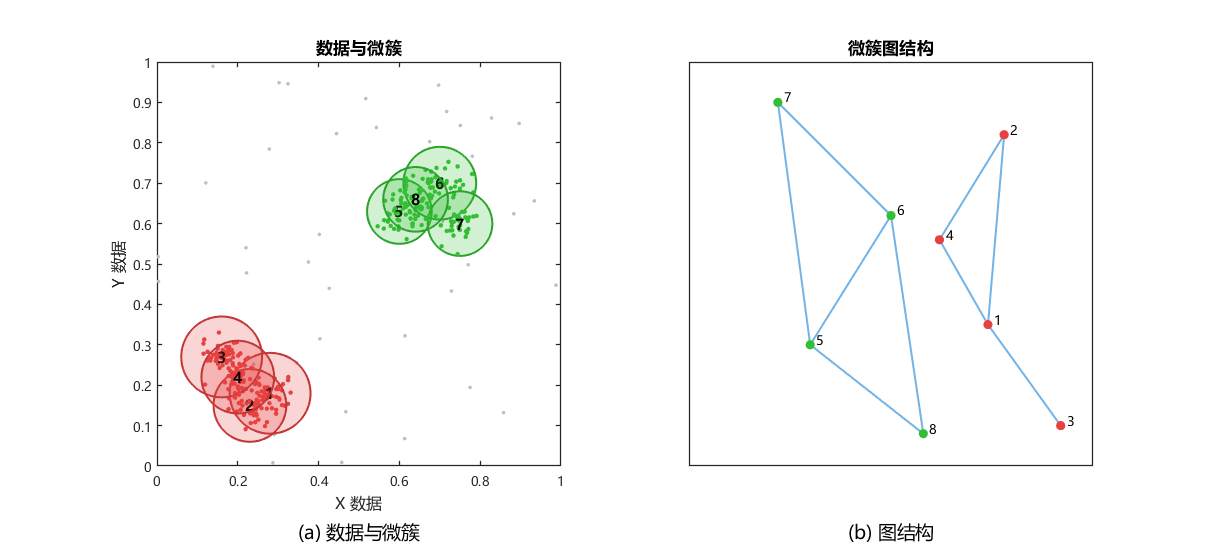
\includegraphics[width=0.85\textwidth]{images/chapter2/CEDAS}
	\caption{CEDAS微簇与图结构示意图}
	\label{fig:cedas_graph}
\end{figure}

从应用角度看，两阶段方法更适合以摘要管理和延迟分析为主的任务，完全在线方法则更适合需要持续输出当前结果的场景。对于本文所面对的地磁事件流而言，后台处理端需要随着数据到达不断维护簇结构和中间结果，难以依赖额外的离线重聚类过程，因此其处理需求更接近完全在线聚类框架。这也是后续章节在设计面向长缺测工况的轨迹重构方法时，更关注在线归并、状态更新和生命周期管理等机制的原因。

\section{本章小结}
本章围绕多地磁传感器车辆目标跟踪的理论基础展开。首先介绍了地磁传感器的车辆检测机理与事件化输出过程，说明地磁扰动如何转化为可用于跟踪的离散检测记录；随后给出了系统架构、双车道部署模型与测量模型，并结合理想与非理想数据流形态分析了漏检、虚警、时间戳误差和迟到到达等主要不确定性来源。在此基础上，进一步梳理了卡尔曼滤波、数据关联以及数据流聚类的基本方法，分别说明了状态估计、量测匹配和在线簇维护在多目标跟踪中的作用。上述内容为后续章节开展在线车辆目标跟踪与长缺测条件下的轨迹重构方法设计奠定了理论与建模基础。


\chapter{复杂交通情况下的双车道多车辆目标跟踪算法}
\label{chap:online_tracking}

\section{引言}

在单向双车道高速公路路段内，基于多地磁传感器的车辆目标跟踪系统会受到数据随机延迟到达、漏检以及噪声干扰等非理想因素的影响；同时，由于车辆行驶行为复杂，邻道干扰与双车长距离并行通过在上报量测的时空特性上又具有较强相似性，难以简单依据单条量测特征判断区分，从而影响车辆实时跟踪的准确性与稳定性。因此，本章面向系统常态工况下存在的量测到达时序错乱、短时漏检、噪声干扰以及复杂并行车况，提出一种基于地磁传感器状态自适应与场景概率判别的在线多车辆目标跟踪方法。

具体而言，本章首先在量测进入关联与滤波之前，利用时间窗口缓存对量测到达时序进行矫正，并通过固定滞后窗口接纳迟到到达的量测，在必要时触发局部回放，从而提高轨迹可利用信息的完整性。其次，在量测时序矫正的基础上，建立与双车道地磁事件流相匹配的车辆运动模型与观测模型，给出状态初始化、状态预测与量测更新方法，形成统一的事件级状态估计框架。随后，围绕多车辆目标的数据关联问题，依次构建跟踪波门、关联似然与软关联权重计算方法，并结合地磁传感器检测概率与杂波强度的在线估计提升复杂工况下的关联鲁棒性；同时，针对邻道干扰与真实双车并行易混淆的问题，引入三状态场景判别模型，对局部交通场景进行概率解释。最后，在轨迹管理阶段，结合目标存在概率递推与基于场景后验的车道状态更新机制，实现轨迹的起始、确认、维持、删除以及车道状态修正，形成完整的在线跟踪流程。

\section{多地磁传感器部署模型及系统介绍}\label{sec:ch2_platform}

相比单个地磁传感器，多地磁传感器协同检测具有更好的可靠性和覆盖能力。沿道路连续布设多个地磁传感器后，车辆在不同观测位置的通过信息可以被依次记录；即使个别地磁传感器受干扰影响而暂时失效，其余地磁传感器的检测数据仍可支撑系统正常运行。与此同时，车辆在某一检测时刻的位置可近似视为对应地磁传感器的预设安装位置，因此联合多点检测数据能够为车辆运动状态估计提供更充分的时空约束。为开展后续车辆目标跟踪研究，下面分别介绍系统架构、地磁传感器部署模型及测量模型。

\subsection{系统架构}

本文搭建了由地磁传感器、数据传输模块、后台处理模块和前端展示模块组成的多地磁车辆感知系统，其总体结构如图~\ref{fig:ch2_system_architecture}所示。系统前端负责车辆检测数据采集，中间层负责多点数据汇聚与回传，后台负责数据接入、处理以及车辆目标跟踪结果输出，前端展示模块负责对跟踪结果进行可视化展示。

\begin{figure}[H]
	\centering
	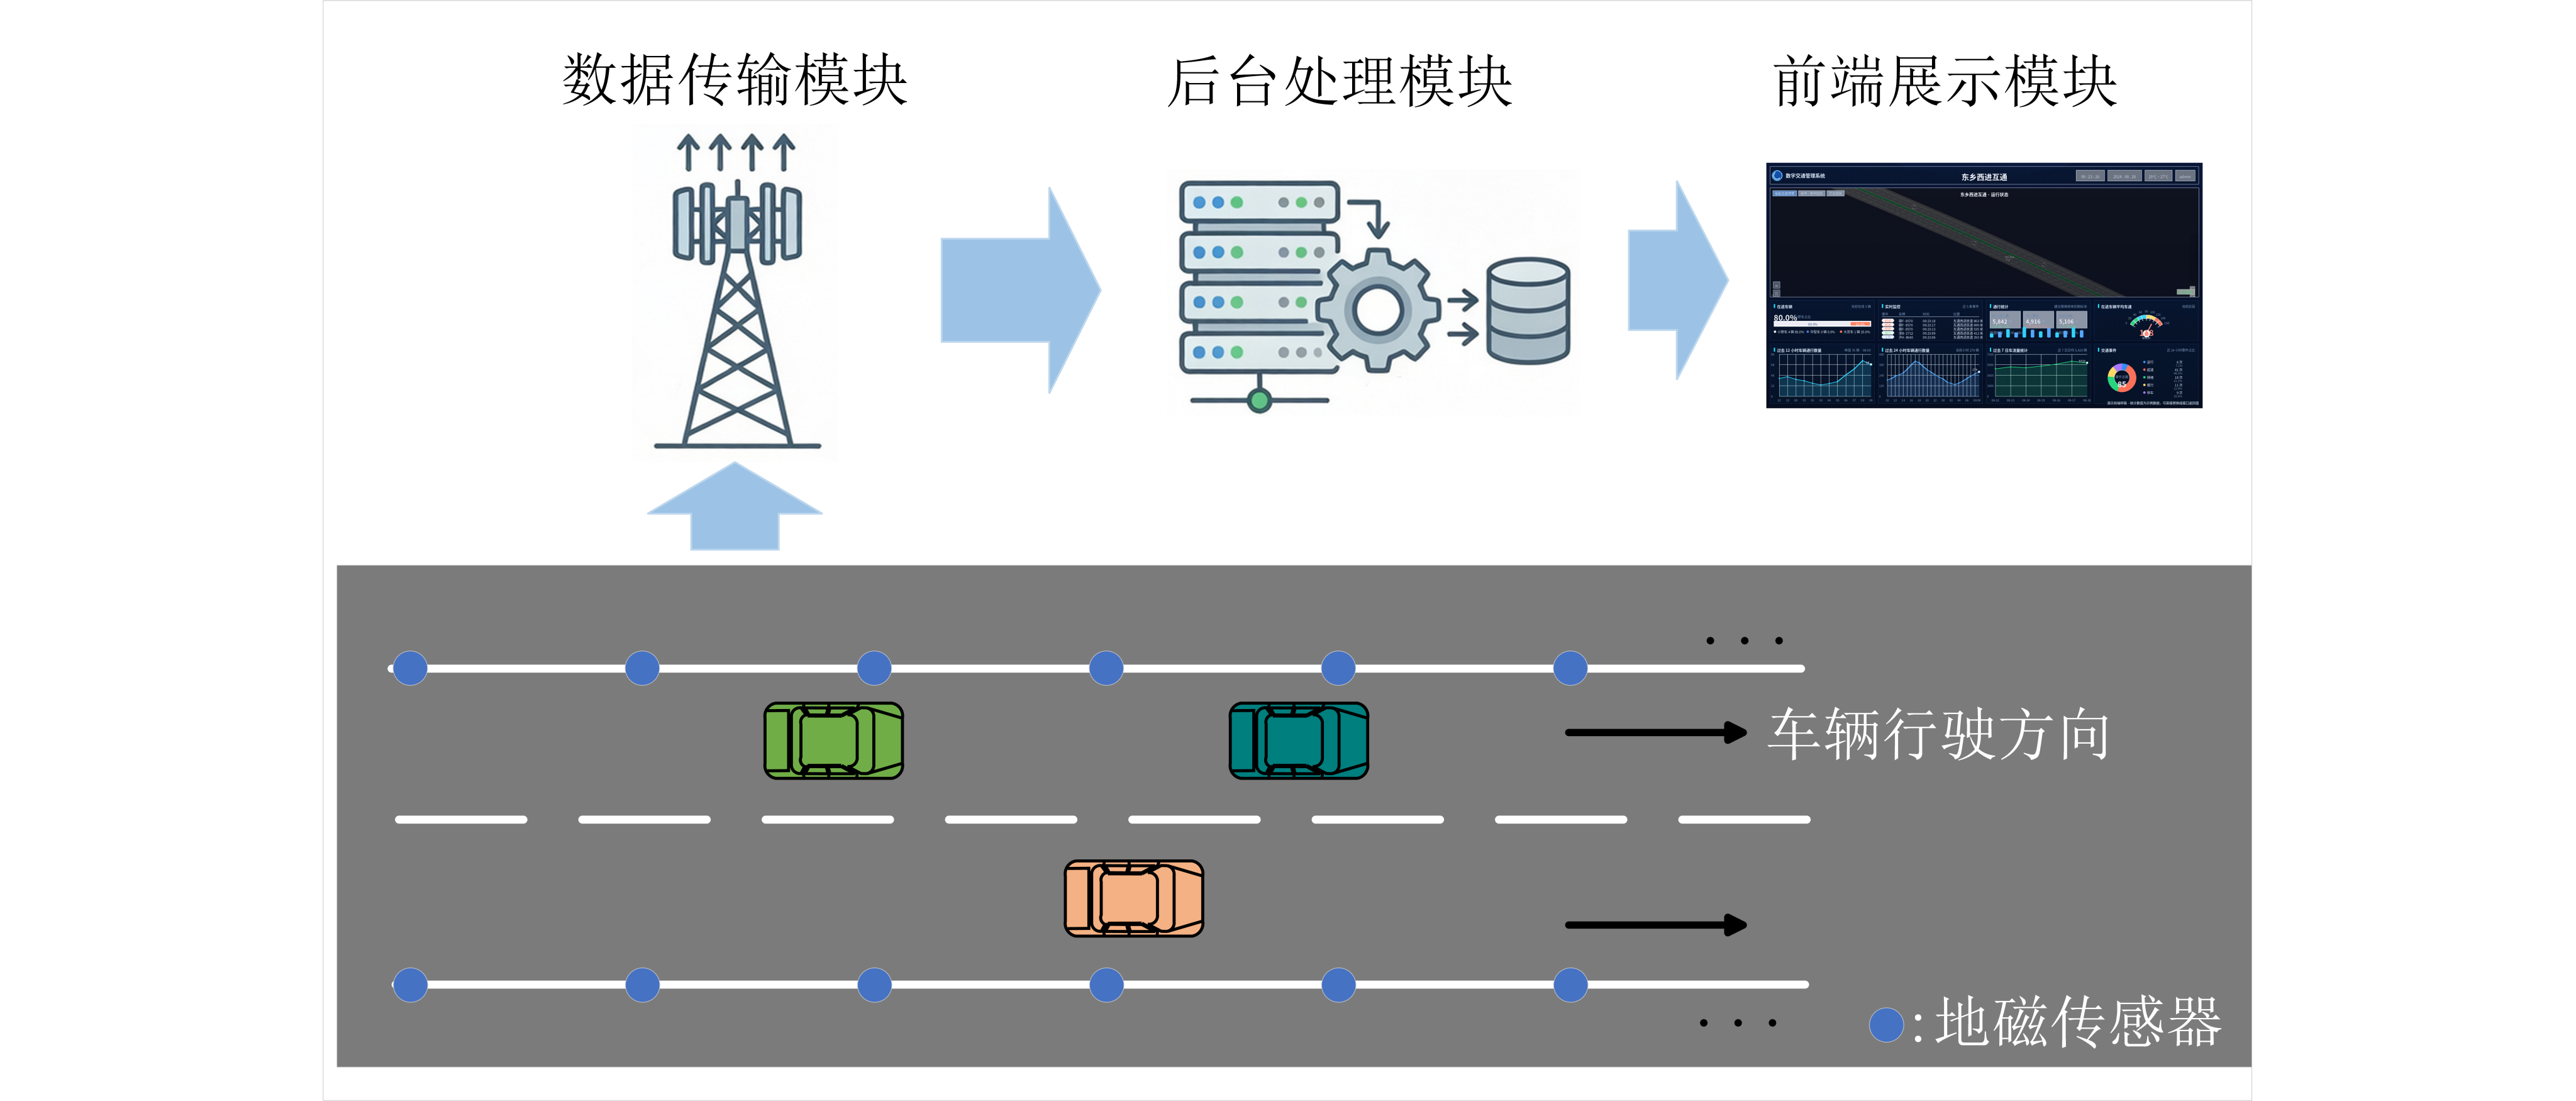
\includegraphics[width=0.9\textwidth]{images/chapter2/fig_2_5_system_v1.png}
	\caption{多地磁传感器车辆目标跟踪系统架构}
	\label{fig:ch2_system_architecture}
\end{figure}

首先，前端地磁传感器负责连续采集路面附近的磁场变化并检测车辆通过。本系统采用一体化地磁传感器设计，将三轴地磁传感器 VCM5883、微控制单元（Micro Control Unit, MCU）、LoRa 通信模块以及太阳能供电与充电单元集成在同一设备中，实物如图~\ref{fig:ch2_geomagnetic_sensor_real}所示。VCM5883 持续输出三轴磁场数据，MCU 在端侧完成必要的预处理、阈值判别和状态机检测，并在车辆通过后生成检测数据。单条检测数据通常包含车辆经过对应地磁传感器的触发时间、地磁传感器编号以及车辆所引起的磁场扰动峰值等字段。生成后的检测数据经 LoRa 通信模块上传至数据传输模块；太阳能供电与充电单元则用于保障地磁传感器在无外接电源条件下的长期稳定运行。

\begin{figure}[H]
	\centering
	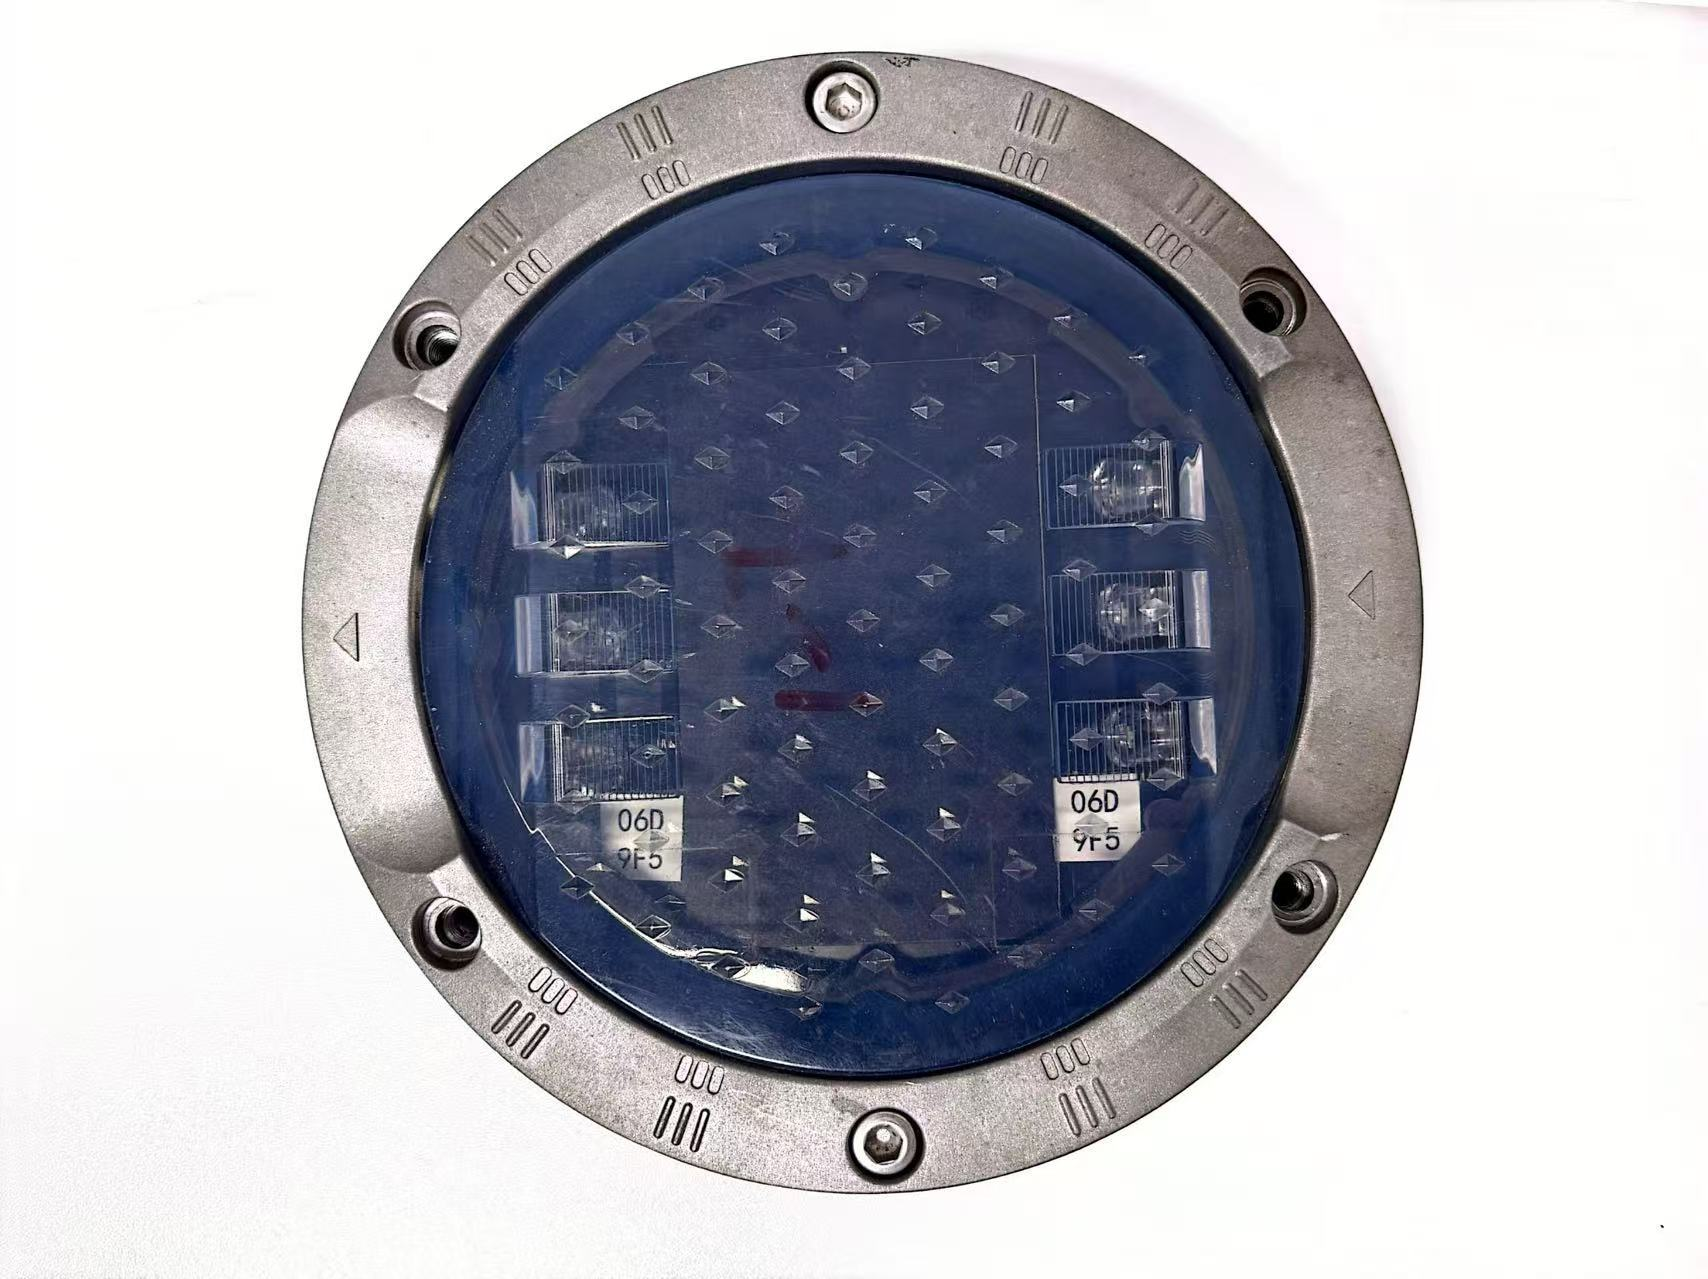
\includegraphics[width=0.45\textwidth]{images/chapter2/fig_2_4_geomagnetic_sensor}
	\caption{地磁传感器实物图}
	\label{fig:ch2_geomagnetic_sensor_real}
\end{figure}

其次，数据传输模块负责多点检测数据的汇聚与回传，其实物如图~\ref{fig:ch2_comm_base_real}所示。该模块一方面可通过 LoRa 与沿线部署的多个地磁传感器建立无线通信，接收并缓存各地磁传感器上传的检测数据；另一方面可通过 4G 网络按预设时间间隔将检测数据打包发送至后台处理模块，从而实现前端检测数据的集中回传。考虑到实际道路环境中的通信条件变化，LoRa 的有效通信距离一般为 3$\sim$5 km。需要说明的是，检测数据流在后台侧按到达顺序进入处理链路，受无线链路时延与回传机制影响，部分量测可能出现随机延迟甚至迟到到达，导致数据到达顺序与实际触发时间顺序不一致，从而对后续关联与更新产生直接影响。

\begin{figure}[H]
	\centering
	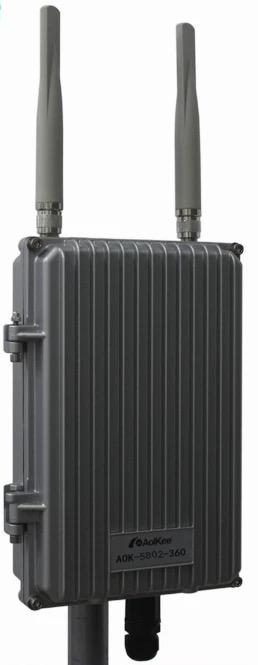
\includegraphics[width=0.15\textwidth]{images/chapter2/fig_2_1_base}
	\caption{数据传输模块实物图}
	\label{fig:ch2_comm_base_real}
\end{figure}

再次，后台处理模块负责对上传的检测数据进行统一接入与处理，本文目前采用云服务器作为后台载体。后台首先完成数据解析与字段校验，随后结合数据关联、状态估计和车道判别等处理，对车辆在路段内的运动状态及行驶车道进行递推估计，最终输出连续的车辆目标跟踪结果。

最后，前端展示模块负责对后台输出的车辆目标跟踪结果进行实时展示。后台处理模块完成车辆实时位置计算后，将车辆位置、所属车道及相关运行信息推送至前端界面，前端据此对路段内车辆运行状态和系统工作状态进行可视化展示。本文搭建的前端展示界面如图~\ref{fig:ch2_online_platform}所示。

\begin{figure}[H]
	\centering
	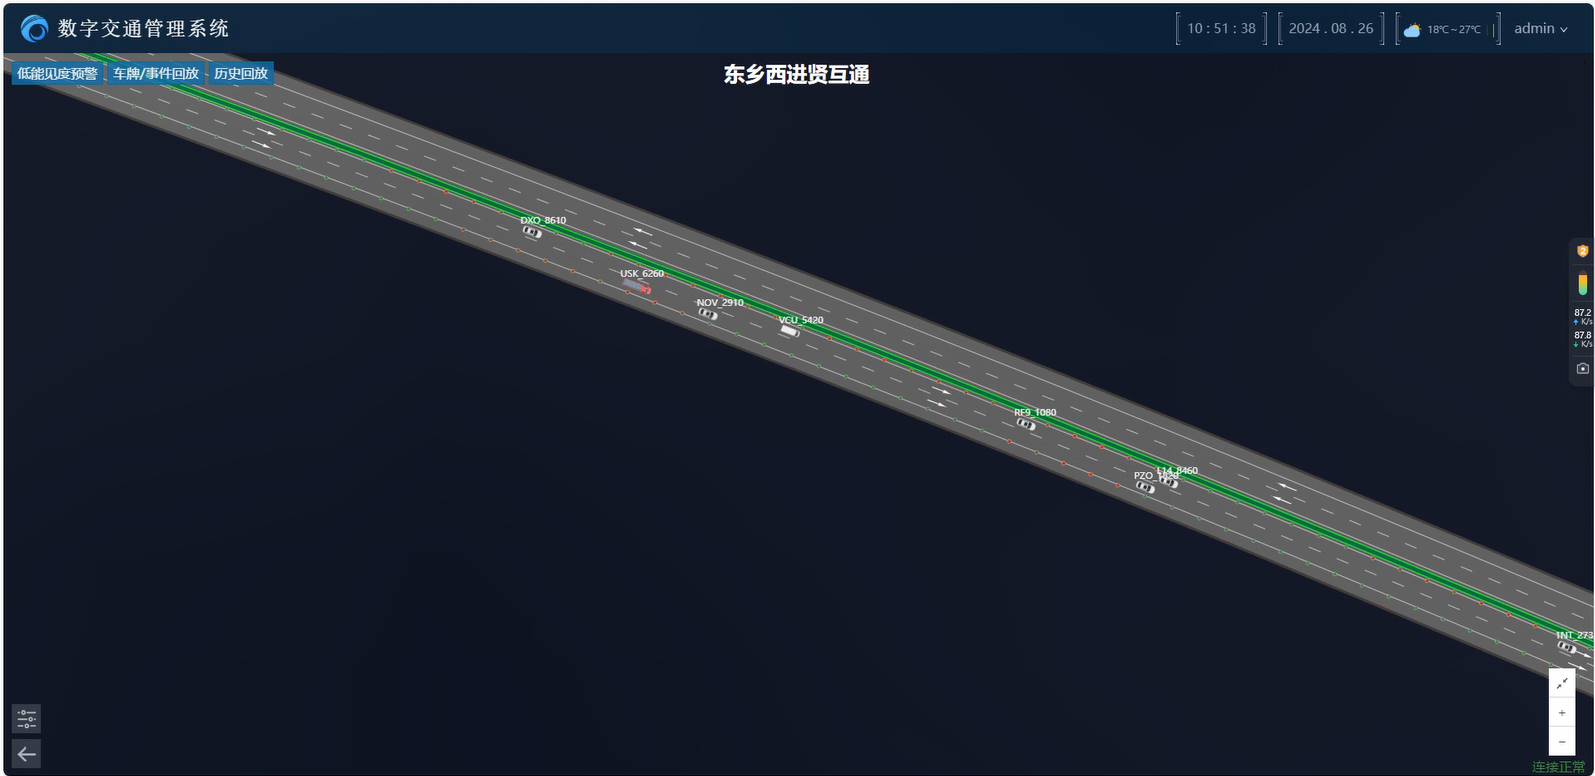
\includegraphics[width=0.85\textwidth]{images/chapter2/fig_2_7_platform}
	\caption{车辆目标跟踪前端展示界面}
	\label{fig:ch2_online_platform}
\end{figure}

\subsection{双车道多地磁传感器部署模型}\label{sec:ch2_summary}

图~\ref{fig:ch2_road_layout}给出了本文研究的单向双车道场景及地磁传感器部署方式。为获得可用于车辆目标跟踪的离散量测序列，本文沿车辆行驶方向以固定纵向间距设置多个观测位置；在每个观测位置的两侧边界车道线附近各部署一个地磁传感器，从而形成左右成对的观测点。图中实心圆点表示地磁传感器。车辆沿纵向行驶时，会依次在不同观测位置形成检测记录，这为后续速度估计、数据关联和轨迹构建提供了基础输入。

\begin{figure}[H]
	\centering
	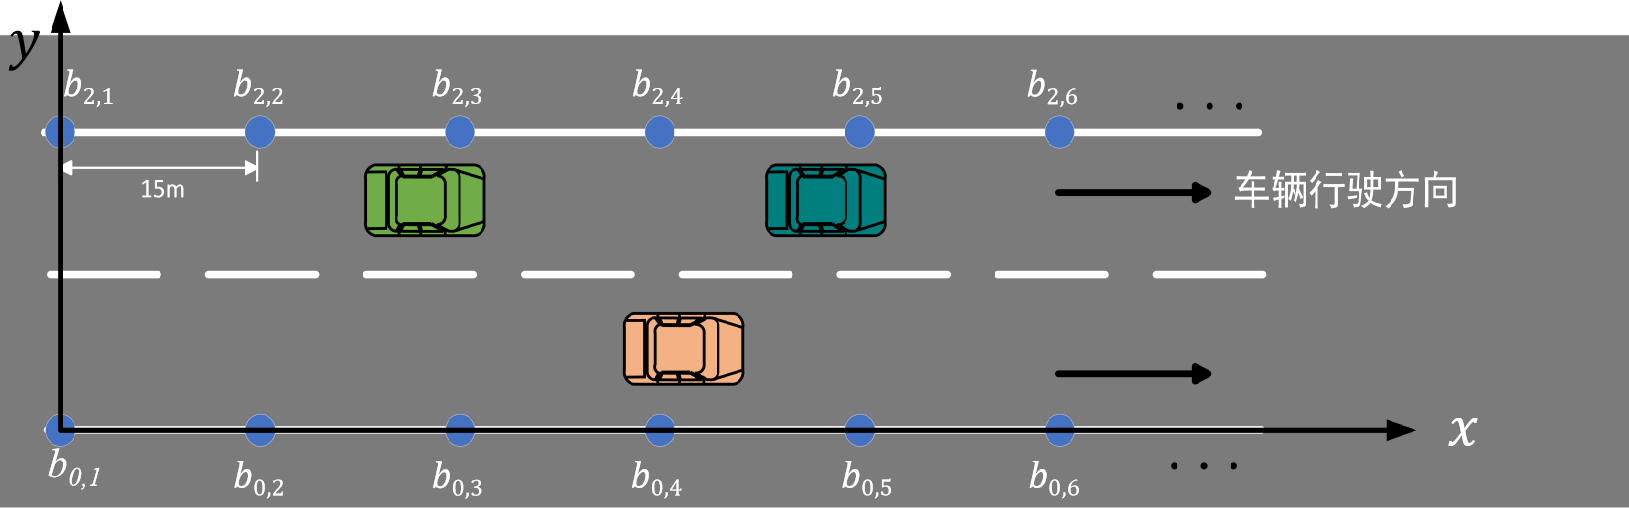
\includegraphics[width=0.85\textwidth]{images/chapter2/fig_2_8_roadv2}
	\caption{单向双车道场景地磁传感器部署示意图}
	\label{fig:ch2_road_layout}
\end{figure}

为便于后续建模与推导，建立道路坐标系：以车辆行驶方向为 $x$ 轴正方向，以横向跨车道方向为 $y$ 轴正方向，并取上游第一组地磁传感器所在的纵向观测位置为坐标原点。本文仅考虑在两条边界车道线附近布设地磁传感器，并与后续车道线索引保持一致，将两条布设车道线编号为

\begin{equation}
	l \in \{0,2\},
	\label{eq:ch2_lane_index}
\end{equation}

其中，$l=0$ 表示左侧边界车道线，$l=2$ 表示右侧边界车道线。沿行驶方向的观测位置按组编号记为

\begin{equation}
	r = 0,1,\ldots,R-1,
	\label{eq:ch2_group_index}
\end{equation}

则位于车道线 $l$ 且属于第 $r$ 组观测位置的地磁传感器记为 $b_{l,r}$。地磁传感器的空间位置用二维坐标向量表示为

\begin{equation}
	\mathbf{s}_{l,r} =
	\begin{bmatrix}
		x_r \\
		y_l
	\end{bmatrix},
	\qquad
	l\in\{0,2\},\; r=0,1,\ldots,R-1,
	\label{eq:ch2_sensor_position}
\end{equation}

其中，$x_r$ 为第 $r$ 个纵向观测位置的坐标，$y_l$ 为对应边界车道线的横向坐标。本文采用对称布设方式，即同一组中的 $b_{0,r}$ 与 $b_{2,r}$ 位于同一纵向观测位置，二者具有相同的 $x_r$，仅在横向位置 $y$ 上不同。相邻两组观测位置的纵向间距记为 $L_a$，则有

\begin{equation}
	x_r = x_0 + rL_a,
	\qquad r=0,1,\ldots,R-1,
	\label{eq:ch2_sensor_spacing}
\end{equation}

其中，$x_0$ 为第一组观测位置的纵向坐标，后续推导中通常取 $x_0=0$ 以简化表达。

需要指出的是，对称布设在工程实现与空间标定上较为直接，但在双车道并行行驶或换道条件下也会提高数据关联难度：一方面，同一纵向观测位置同时存在左右两个观测点，不同车辆的检测时间可能相互接近甚至部分重叠；另一方面，车辆横向位置变化会使左右地磁传感器的触发时间和扰动强度产生偏移，因此仅依据时空邻近关系往往难以稳定完成对应匹配。基于上述部署模型，下一节将给出量测的统一表示，并结合理想与非理想检测数据流说明后续跟踪中面临的主要不确定性。

\subsection{双车道多地磁传感器测量模型}

当地磁传感器检测到车辆通过后，系统会向后台上传一条检测数据。将后台按到达顺序接收的第 $j$ 条检测数据记为量测向量 $\mathbf z_j$，结合本文系统的上报格式，量测可定义为

\begin{equation}
	\mathbf z_j=
	\begin{bmatrix}
		t_j &
		b_j &
		x_{b_j} &
		y_{b_j} &
		l_{b_j} &
		Mpeak_j
	\end{bmatrix}^{\mathrm T},
	\label{eq:ch2_measurement_vector}
\end{equation}

其中，$t_j$ 为触发时间戳，$b_j$ 为地磁传感器设备编号，$x_{b_j}$ 和 $y_{b_j}$ 分别为该设备在道路坐标系下的纵向和横向安装坐标，$l_{b_j}$ 为该设备所属边界车道线编号，$Mpeak_j$ 为对应车辆引起的磁场扰动峰值。式~\eqref{eq:ch2_measurement_vector}描述了车辆在时刻 $t_j$ 于观测点 $(x_{b_j},y_{b_j})$ 附近形成的一次离散量测。


\textnormal{(1) 理想检测数据流形态}\par\vspace{0.3\baselineskip}

图~\ref{fig:ch2_detection_flow}中的(a)给出了理想情况下检测数据流的典型形态。图中以时间戳为横轴、设备编号为纵轴，每一个散点对应一条检测记录。

\begin{figure}[H]
	\centering
	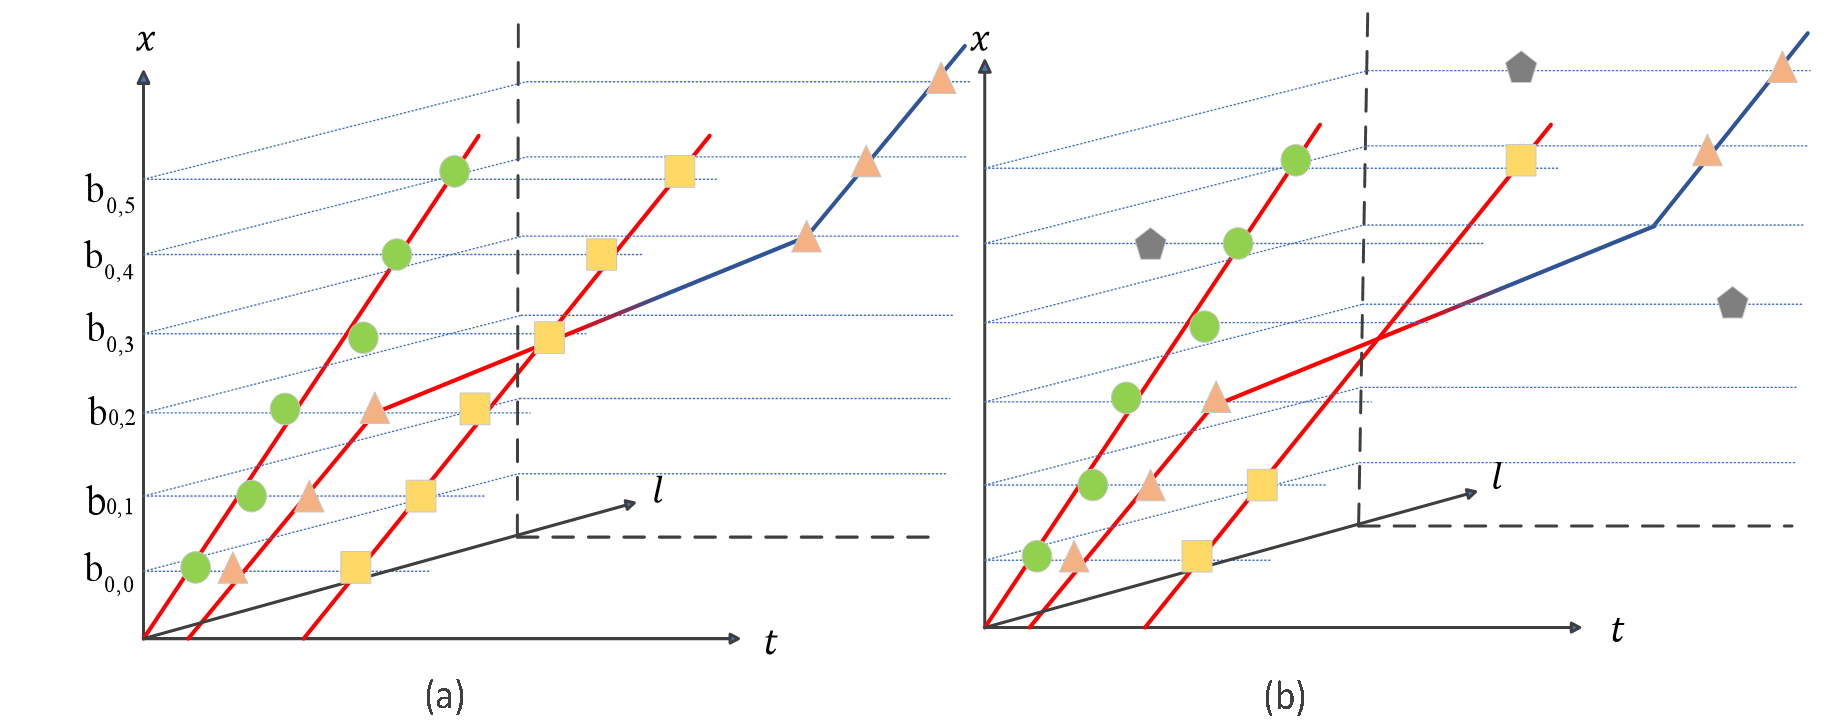
\includegraphics[width=0.85\textwidth]{images/chapter2/fig_2_9_data_v2}
	\caption{地磁传感器检测数据在理想与非理想情况下的分布}
	\label{fig:ch2_detection_flow}
\end{figure}

如图所示，同一车辆沿路段向下游行驶时，其量测点会随着纵向布设顺序依次出现在更下游的地磁传感器上，在 $\text{Time--SensorID}$ 平面内呈现近似单调上升的轨迹结构。当车速变化不剧烈时，同一车辆在相邻两个纵向观测位置处的触发时间差满足近似关系

\begin{equation}
	t_{r+1}-t_r \approx \frac{L_a}{v},
	\label{eq:ch2_time_interval}
\end{equation}

其中，$t_r$ 表示同一车辆在第 $r$ 个纵向观测位置处的触发时间，$L_a$ 为相邻观测位置的纵向间距，$v$ 为车辆纵向速度。由此可见，在理想条件下，检测数据在时间轴和空间轴上具有较强的连续性，这为后续门控与数据关联提供了重要先验。进一步地，当车辆保持当前车道直行时，其量测点通常会持续出现在同一侧地磁传感器序列上；而当车辆发生换道时，量测点则会在两侧地磁传感器序列之间出现切换或过渡。


\textnormal{(2) 非理想检测数据流形态}\par\vspace{0.3\baselineskip}

真实道路环境下，检测数据流通常表现为图~\ref{fig:ch2_detection_flow}中的(b)所示的非理想形态，与理想情况相比主要差异可归纳为以下三类。

首先是漏检导致的量测缺失。部分观测位置未形成有效检测记录，既可能表现为单次缺失，也可能在若干相邻观测位置上连续缺失，从而使同一车辆的量测点出现明显空档并导致轨迹结构断裂。这会直接削弱由时间差推得的速度约束，并增大后续关联的不确定性。

其次是虚警导致的杂波量测。相邻车道干扰、环境噪声或异常电磁扰动可能产生与真实车辆无关的检测点，这些检测点通常分布较为离散，且缺乏与真实车辆一致的时空连续性。当车流密度较高时，这类杂波量测会显著扩大候选关联集合，增加误关联风险。

最后是时间戳误差与迟到到达。不同地磁传感器之间的时钟偏差，以及无线链路回传过程中的随机时延，都会使同一车辆在不同观测位置形成的检测数据在时间轴上出现错位甚至局部乱序，从而增加时序组织与状态更新的难度。

因此，本文所研究的多地磁传感器车辆目标跟踪问题，本质上是在存在漏检、虚警、时间戳偏差及迟到量测等不确定因素的条件下，利用多点检测数据完成车辆量测关联，并进一步估计车辆的运动状态与行驶车道。后续章节将在此基础上展开具体算法设计。




\section{量测时序矫正}

道路侧多地磁传感器在车辆触发后，会将检测事件上报至后台处理模块。然而在实际部署中，地磁传感器上传链路容易受到网络波动、通信排队以及异步传输等因素影响，从而产生随机时延，使得部分量测的到达顺序与车辆在道路上真实触发各地磁传感器的先后顺序并不一致。若系统直接按照量测到达顺序进行在线处理，则某些“触发较早但到达较晚”的量测会被暂时跳过，算法只能基于不完整的事件序列先行完成跨地磁传感器数据关联，这不仅会增加候选匹配的不确定性和关联歧义，也会削弱后续状态预测与轨迹维护的可靠性。

进一步地，当迟到量测在关联与更新完成后才到达时，目标轨迹往往已经沿时间轴推进到更靠后的位置。此时，该量测一方面可能被错误地吸收为后方邻近车辆的观测，引发错误关联并干扰后续车辆的关联判断；另一方面也可能因与当前轨迹的时空位置不再一致而被直接舍弃，造成有效量测浪费。因此，在量测进入状态估计与数据关联模块之前，有必要首先对到达事件进行时序矫正，在有限滞后范围内尽可能恢复量测的真实触发顺序，从而为后续跨地磁传感器关联提供时间一致且信息尽可能完整的输入。

\subsection{基于时间窗口缓存的量测时序重排}

沿用第2章对单条地磁事件量测的定义，这里仍将后台接收到的第 $j$ 条记录记为
\begin{equation}
	\mathbf z_j=
	\begin{bmatrix}
		t_j &
		b_j &
		x_{b_j} &
		y_{b_j} &
		l_{b_j} &
		Mpeak_j
	\end{bmatrix}^{\mathrm T},
	\label{eq:ch3_event_def}
\end{equation}
其中，$t_j$ 为触发时间戳，$b_j$ 为触发地磁传感器编号，$x_{b_j}$ 和 $y_{b_j}$ 分别为地磁传感器 $b_j$ 在道路坐标系下的纵向与横向安装坐标，$l_{b_j}$ 为该地磁传感器对应的边界车道线编号，$Mpeak_j$ 为地磁扰动峰值。为便于后续书写，下面将 $l_{b_j}$ 简记为 $l_j$。在本节中，时间窗口缓存并不是新的时间刻度，而是一个按固定时间片组织的短时缓存区：缓存中的每一个槽位对应一个扫描，所有新到达量测先根据触发时间被写入相应槽位，再在缓存内完成排序和后续处理。因此，后文所说的“扫描序号”，也就是量测在时间窗口缓存中的槽位编号。

给定参考时刻 $t_0$，事件 $\mathbf z_j$ 所属的扫描序号定义为
\begin{equation}
	n(j)=\left\lfloor \frac{t_j-t_0}{\Delta T} \right\rfloor +1.
	\label{eq:ch3_scan_index}
\end{equation}
其中，$\Delta T$ 为时间窗口缓存的扫描时间片长度，其取值通常结合系统允许的处理时延、输出刷新要求以及迟到量测延迟分布的统计结果共同设定。于是，第 $n$ 个扫描内的量测集合可写为
\begin{equation}
	\mathcal Z_n=
	\left\{
	\mathbf z_j\,\big|\, n(j)=n
	\right\}.
	\label{eq:ch3_scan_set}
\end{equation}
时间窗口缓存本质上就是按扫描序号排列的若干个量测集合，系统在线处理时只维护其中最近一段时间内的扫描槽位，从而既保留了时间先后关系，也为迟到量测回插预留了位置。

同一扫描内，不同地磁传感器上报的量测到达顺序仍可能与真实触发顺序不一致，因此还需要在扫描内部按触发时间戳升序排序，得到
\begin{equation}
	\mathcal Z_n^{\uparrow}=\mathrm{Sort}\left(\mathcal Z_n; t_j\uparrow\right).
	\label{eq:ch3_scan_sort}
\end{equation}
后续的状态预测、量测关联和轨迹更新均按照 $\mathcal Z_n^{\uparrow}$ 中的顺序逐条执行。这样，系统先在扫描层面对事件作粗粒度对齐，再在扫描内部恢复真实先后关系，使进入后续递推的事件流在时间上尽可能一致。

\subsection{基于固定滞后窗口的局部处理结果回退}

扫描内排序可以解决同一扫描中的局部乱序，但仍不能处理跨扫描迟到到达的量测。若某条量测在其真实触发扫描已经处理完成后才到达系统，直接忽略它，或者将其并入当前扫描，都会破坏已有轨迹的时间一致性。为此，在时间窗口缓存上进一步引入固定滞后窗口，对最近 $L$ 个扫描保持可回溯状态。定义时刻 $n$ 的活动窗口为
\begin{equation}
	\mathcal W_n=
	\left\{
	\mathcal Z_{n-L+1},\ldots,\mathcal Z_n
	\right\}.
	\label{eq:ch3_lag_window}
\end{equation}
同时，在窗口左端保留快照状态
\begin{equation}
	\mathcal S_{n-L}=
	\left\{
	\hat{\mathbf x}_{i,k|k},\mathbf P_{i,k|k},P_{E,i},
	\boldsymbol\pi_i^{\mathrm{lane}},
	\boldsymbol\pi_g^{\mathrm{scene}},
	\alpha_{D,b},\beta_{D,b},a_{\lambda_c,b},b_{\lambda_c,b}
	\right\},
	\label{eq:ch3_snapshot_reorg}
\end{equation}
其中，$k=n-L$ 表示窗口左端之前最近一次已定稿的时刻；$\hat{\mathbf x}_{i,k|k}$ 和 $\mathbf P_{i,k|k}$ 分别为轨迹 $i$ 在该时刻的后验状态估计与协方差，$P_{E,i}$ 为轨迹存在概率，$\boldsymbol\pi_i^{\mathrm{lane}}$ 为轨迹 $i$ 的车道后验向量，$\boldsymbol\pi_g^{\mathrm{scene}}$ 为地磁传感器对 $g$ 的场景后验向量，$\alpha_{D,b}$ 与 $\beta_{D,b}$ 为地磁传感器 $b$ 检测概率的 Beta 后验参数，$a_{\lambda_c,b}$ 与 $b_{\lambda_c,b}$ 为地磁传感器 $b$ 杂波空间密度的 Gamma 后验参数。之所以需要同时保留这些信息，是因为局部回放不仅要回退轨迹运动状态，还要恢复当时用于关联、场景判别和地磁传感器状态更新的先验条件，这样重新执行窗口内各扫描时，才能与原始处理链条保持一致。

当新到达量测 $\mathbf z_j$ 满足
\begin{equation}
	n(j)\in\{n-L+1,\ldots,n\},
	\label{eq:ch3_late_condition}
\end{equation}
则认为其属于固定滞后窗口内的迟到量测。此时，系统先将该量测回插至对应历史扫描的量测集合中，再从快照 $\mathcal S_{n-L}$ 出发，将该快照之后已经生成的关联、状态更新和轨迹管理结果全部回退，并按时间顺序重新执行窗口内的状态预测、场景判别、数据关联、量测更新和轨迹管理流程。若量测所属扫描早于窗口左端，则说明其已超出当前在线可修正范围，不再纳入在线跟踪流程。借助固定滞后窗口与局部回放机制，系统可以利用后续到达的信息对近期历史关联结果进行局部修正，在不过度增加计算开销的前提下，改善短时乱序和迟到条件下的轨迹连续性与结果一致性。

\section{基于双车道多地磁传感器数据的车辆状态估计算法}
\label{sec:ch3_state_estimation}

完成量测时序矫正后，系统获得了按真实触发时间组织的地磁传感器数据流输入。接下来需要在此基础上建立与地磁事件流相匹配的车辆状态估计算法，把车辆在某一时刻通过某一已知地磁传感器的离散检测事实转化为可递推的状态约束，为后续的数据关联、场景判别和轨迹管理提供统一的状态表达。由于地磁量测本质上仍是离散事件，而不是可直接使用的连续轨迹状态，本节按照模型建立、状态初始化、状态预测和量测更新的顺序给出事件级状态估计方法。



\subsection{车辆运动模型与量测模型}

由于双车道地磁系统并不直接提供车辆横向连续坐标，本文仅对车辆沿道路纵向的连续状态进行递推估计，而将横向安装位置、边界车道线编号和地磁扰动峰值等信息作为离散证据保留，用于后续的数据关联与车道状态判别。考虑到车辆在高速路段沿车道纵向行驶，且相邻地磁传感器之间的通过时间通常处于较短时间尺度内，本文采用常速度（CV）模型作为车辆纵向运动的基础模型。设轨迹 $i$ 在第 $k$ 次有效更新后的状态向量为
\begin{equation}
	\mathbf x_{i,k}=
	\begin{bmatrix}
		p_{i,k}\\
		v_{i,k}
	\end{bmatrix},
	\label{eq:ch3_state_vec}
\end{equation}
其中，$p_{i,k}$ 与 $v_{i,k}$ 分别表示车辆在道路纵向上的位置与速度。

若轨迹 $i$ 在相邻两次有效更新之间的时间间隔为 $\Delta t_{i,k+1}$，则其状态转移模型写为
\begin{equation}
	\mathbf x_{i,k+1}=
	\mathbf F\left(\Delta t_{i,k+1}\right)\mathbf x_{i,k}+\mathbf w_{i,k},
	\label{eq:ch3_state_transition}
\end{equation}
其中，状态转移矩阵为
\begin{equation}
	\mathbf F\left(\Delta t_{i,k+1}\right)=
	\begin{bmatrix}
		1 & \Delta t_{i,k+1}\\
		0 & 1
	\end{bmatrix},
	\label{eq:ch3_F}
\end{equation}
过程噪声满足 $\mathbf w_{i,k}\sim\mathcal N(\mathbf 0,\mathbf Q(\Delta t_{i,k+1}))$。考虑短时机动和时间戳抖动对纵向传播误差的影响，过程噪声协方差写为
\begin{equation}
	\mathbf Q\left(\Delta t_{i,k+1}\right)
	=
	q_a
	\begin{bmatrix}
		\dfrac{\Delta t_{i,k+1}^{4}}{4} & \dfrac{\Delta t_{i,k+1}^{3}}{2}\\[6pt]
		\dfrac{\Delta t_{i,k+1}^{3}}{2} & \Delta t_{i,k+1}^{2}
	\end{bmatrix}
	+
	\begin{bmatrix}
		c_t \hat v_{i,k+1|k}^{\,2}\sigma_t^2 & 0\\
		0 & 0
	\end{bmatrix}.
	\label{eq:ch3_Q}
\end{equation}

当地磁事件最终被关联到轨迹后，事件"车辆在时刻 $t_j$ 通过地磁传感器 $b_j$"这一事实可转化为纵向位置约束。记地磁传感器 $b_j$ 的纵向安装坐标为 $x_{b_j}$，则定义伪位置观测
\begin{equation}
	\tilde p_{i,k+1}=x_{b_j}.
	\label{eq:ch3_pseudo_meas}
\end{equation}
相应的观测模型写为
\begin{equation}
	\tilde p_{i,k+1}=\mathbf H\mathbf x_{i,k+1}+e_{i,k+1},
	\qquad
	\mathbf H=
	\begin{bmatrix}
		1 & 0
	\end{bmatrix},
	\qquad
	e_{i,k+1}\sim\mathcal N(0,R_{b_j}),
	\label{eq:ch3_measurement_k}
\end{equation}
其中，$R_{b_j}$ 为与地磁传感器 $b_j$ 相关的观测方差。需要说明的是，$R_{b_j}$ 反映的是地磁传感器触发区间宽度、安装标定误差以及地磁传感器工作状态不稳定性折算到位置约束上的不确定性，而不是时间戳误差方差。后文将根据地磁传感器检测概率与杂波强度的在线估计结果，对 $R_{b_j}$ 进行自适应调整。

\subsection{状态初始化}

新生轨迹只对当前扫描中未被任何已确认轨迹吸收的量测执行初始化，而不会反过来参与当前时刻已有轨迹的关联竞争。设事件 $\mathbf z_{j_0}$ 触发了新候选轨迹 $i$，则其初始位置取为对应地磁传感器的纵向坐标
\begin{equation}
	p_{i,0}=x_{b_{j_0}}.
	\label{eq:ch3_init_pos}
\end{equation}
由于单条地磁事件无法可靠提供速度信息，本文采用道路历史平均速度或经验速度 $\bar v_0$ 作为初始速度先验，从而得到初始状态均值
\begin{equation}
	\hat{\mathbf x}_{i,0|0}=
	\begin{bmatrix}
		p_{i,0}\\
		\bar v_0
	\end{bmatrix}.
	\label{eq:ch3_init_state}
\end{equation}
对应的初始协方差取为
\begin{equation}
	\mathbf P_{i,0|0}=\mathrm{diag}\left(\sigma_{p0}^{2},\sigma_{v0}^{2}\right),
	\label{eq:ch3_init_cov}
\end{equation}
其中，$\sigma_{p0}^{2}$ 与地磁传感器位置观测方差同量级，$\sigma_{v0}^{2}$ 取较大的先验值，以反映新生轨迹在初始阶段速度不确定性较高。

为使地磁扰动峰值信息能够进入后续关联计算，本文同时维护轨迹级对数磁峰值统计量。设新生事件的对数峰值为
\begin{equation}
	m_{i,0}=\log(Mpeak_{j_0}+\varepsilon_M),
	\label{eq:ch3_init_mag}
\end{equation}
则初始化其磁特征均值与方差为
\begin{equation}
	\mu_{i,0}^{M}=m_{i,0},
	\qquad
	(\sigma_{i,0}^{M})^{2}=\sigma_{M0}^{2}.
	\label{eq:ch3_init_mag_stat}
\end{equation}
这样设置的目的在于，使新生轨迹除了具备位置与速度先验外，还保留可供后续关联使用的地磁特征先验。

\subsection{状态预测}

设轨迹 $i$ 在第 $k$ 次有效更新后的后验状态均值与协方差分别为
\begin{equation}
	\hat{\mathbf x}_{i,k|k},
	\qquad
	\mathbf P_{i,k|k}.
	\label{eq:ch3_post_state}
\end{equation}
若后续某条事件最终对应其第 $k+1$ 次有效更新，则该事件触发时间记为 $t_j$，相邻两次有效更新之间的时间间隔定义为
\begin{equation}
	\Delta t_{i,k+1}=t_j-t_{i,k}.
	\label{eq:ch3_dt_update}
\end{equation}
于是，轨迹 $i$ 在第 $k+1$ 次更新前的预测状态均值与预测协方差分别为
\begin{equation}
	\hat{\mathbf x}_{i,k+1|k}
	=
	\mathbf F\left(\Delta t_{i,k+1}\right)\hat{\mathbf x}_{i,k|k},
	\label{eq:ch3_predict_state}
\end{equation}
\begin{equation}
	\mathbf P_{i,k+1|k}
	=
	\mathbf F\left(\Delta t_{i,k+1}\right)
	\mathbf P_{i,k|k}
	\mathbf F^{\mathrm T}\left(\Delta t_{i,k+1}\right)
	+
	\mathbf Q\left(\Delta t_{i,k+1}\right).
	\label{eq:ch3_predict_cov}
\end{equation}
由此可将轨迹状态传播到候选事件触发时刻，为后续量测关联和滤波更新提供统一的预测先验。

\subsection{量测更新}

若轨迹 $i$ 最终被分配到事件 $\mathbf z_j$，则由伪位置观测模型可得创新为
\begin{equation}
	\nu_{i,k+1}=\tilde p_{i,k+1}-\mathbf H\hat{\mathbf x}_{i,k+1|k},
	\label{eq:ch3_innovation_event}
\end{equation}
对应的创新方差为
\begin{equation}
	S_{i,k+1}=\mathbf H\mathbf P_{i,k+1|k}\mathbf H^{\mathrm T}+R_{b_j}.
	\label{eq:ch3_S_event}
\end{equation}
于是，Kalman 增益写为
\begin{equation}
	\mathbf K_{i,k+1}
	=
	\mathbf P_{i,k+1|k}\mathbf H^{\mathrm T}
	\left(
	\mathbf H\mathbf P_{i,k+1|k}\mathbf H^{\mathrm T}+R_{b_j}
	\right)^{-1},
	\label{eq:ch3_K_event}
\end{equation}
相应的状态均值与协方差更新为
\begin{equation}
	\hat{\mathbf x}_{i,k+1|k+1}
	=
	\hat{\mathbf x}_{i,k+1|k}
	+
	\mathbf K_{i,k+1}\nu_{i,k+1},
	\label{eq:ch3_update_state_event}
\end{equation}
\begin{equation}
	\mathbf P_{i,k+1|k+1}
	=
	\left(\mathbf I-\mathbf K_{i,k+1}\mathbf H\right)\mathbf P_{i,k+1|k}.
	\label{eq:ch3_update_cov_event}
\end{equation}
若轨迹在当前扫描内未获得有效关联，则不执行量测更新，而仅保留预测结果，并将该次未命中事实作为后续目标存在概率递推和地磁传感器检测概率统计更新的输入证据。至此，本文建立了与地磁事件流相匹配的事件级状态估计框架。下面进一步解决多车辆共享事件流条件下的量测归属与场景消歧问题。

\section{多车辆目标的数据关联与并行场景判别算法设计}
\label{sec:ch3_association}

在完成车辆状态估计模型之后，下一步需要处理事件流中的量测来源不确定性问题。对于双车道地磁系统而言，量测归属不仅取决于时间一致性，还受到地磁传感器检测能力差异、杂波水平变化以及邻道干扰与真实双车并行混淆的共同影响。因此，本节围绕跟踪波门、关联似然与软关联权重、地磁传感器状态自适应以及并行场景判别四个方面构建统一的概率建模框架。

\subsection{跟踪波门设置}

由于地磁量测在时间轴上异步到达，系统无法像同步采样传感器那样在单一采样时刻统一判断所有事件的来源。因此，本文首先基于时间一致性构造轨迹门控。对任意候选事件 $\mathbf z_j$，记其触发地磁传感器编号为 $b_j$，对应地磁传感器的纵向安装坐标为 $x_{b_j}$，触发时间戳为 $t_j$。若轨迹 $i$ 在当前状态下可能继续前进至该地磁传感器，则由常速度模型可得到其预测通过地磁传感器 $b_j$ 的时刻
\begin{equation}
	\hat t_{i\rightarrow b_j}
	=
	t_{i,k}+\frac{x_{b_j}-\hat p_{i,k|k}}{\hat v_{i,k|k}}.
	\label{eq:ch3_pred_time}
\end{equation}
于是，事件 $\mathbf z_j$ 与轨迹 $i$ 之间的时间残差定义为
\begin{equation}
	\nu^{t}_{i,j}=t_j-\hat t_{i\rightarrow b_j}.
	\label{eq:ch3_time_residual}
\end{equation}
由式~\eqref{eq:ch3_pred_time} 对状态变量 $(p,v)$ 作一阶线性化，可得雅可比向量
\begin{equation}
	\mathbf J_{i,j}
	=
	\begin{bmatrix}
		-\dfrac{1}{\hat v_{i,k|k}} & -\dfrac{x_{b_j}-\hat p_{i,k|k}}{\hat v_{i,k|k}^{\,2}}
	\end{bmatrix},
	\label{eq:ch3_time_jacobian}
\end{equation}
从而时间残差方差写为
\begin{equation}
	S^{t}_{i,j}=\mathbf J_{i,j}\mathbf P_{i,k|k}\mathbf J_{i,j}^{\mathrm T}+\sigma_{t,b_j}^{2},
	\label{eq:ch3_time_var}
\end{equation}
其中，$\sigma_{t,b_j}^{2}$ 表示地磁传感器 $b_j$ 的时间戳误差方差。基于此，定义时间域归一化距离
\begin{equation}
	d^{t\,2}_{i,j}=\frac{\left(\nu^{t}_{i,j}\right)^2}{S^{t}_{i,j}}.
	\label{eq:ch3_time_maha}
\end{equation}
当 $d^{t\,2}_{i,j}\le \gamma_t$ 时，认为事件 $\mathbf z_j$ 落入轨迹 $i$ 的时间门控范围内，其中 $\gamma_t$ 为时间门控阈值。对应的门控宽度可写为
\begin{equation}
	V^{t}_{i,j}=2\sqrt{\gamma_t S^{t}_{i,j}}.
	\label{eq:ch3_gate_width_time}
\end{equation}
该门控机制为后续关联求解提供了候选事件集合，并显著降低了不合理匹配进入关联阶段的概率。

\subsection{标准化关联似然比计算}

在跟踪波门筛选出候选事件之后，本文进一步构造融合运动学一致性、地磁扰动峰值一致性和车道/场景一致性的关联似然。对轨迹 $i$ 与事件 $\mathbf z_j$，定义总似然为
\begin{equation}
	g(\mathbf z_j\mid \hat{\mathbf x}_{i,k|k})
	=
	g_{i,j}^{\mathrm{time}}
	\phi_{i,j}^{\mathrm{mag}}
	\phi_{i,j}^{\mathrm{lane}},
	\label{eq:ch3_total_likelihood}
\end{equation}
其中，基于时间残差的运动学一致性项为
\begin{equation}
	g_{i,j}^{\mathrm{time}}
	=
	\frac{1}{\sqrt{2\pi S^{t}_{i,j}}}
	\exp\left(-\frac{1}{2}d^{t\,2}_{i,j}\right),
	\label{eq:ch3_g_time}
\end{equation}
地磁扰动峰值一致性项采用轨迹历史对数峰值统计建模：
\begin{equation}
	\phi_{i,j}^{\mathrm{mag}}
	=
	\exp\left[
	-\frac{
		\left(
		\log(Mpeak_j+\varepsilon_M)-\mu_i^{M}
		\right)^2
	}{2\left((\sigma_i^{M})^2+\varepsilon_M\right)}
	\right],
	\label{eq:ch3_phi_mag}
\end{equation}
车道/场景一致性项定义为
\begin{equation}
	\phi_{i,j}^{\mathrm{lane}}
	=
	\sum_{l\in\{1,2\}}
	p\!\left(l_j\middle|l,\boldsymbol\pi_{g(j),n}^{\mathrm{scene}}\right)
	\pi_{i,n}^{\mathrm{lane}}(l),
	\label{eq:ch3_phi_lane}
\end{equation}
其中，$g(j)$ 表示事件 $\mathbf z_j$ 所属的左右地磁传感器对编号。

为使不同地磁传感器、不同车流密度和不同杂波条件下的关联代价具有可比性，本文采用显式包含地磁传感器检测概率与地磁传感器杂波空间密度的标准化关联似然比。记事件 $\mathbf z_j$ 所属地磁传感器 $b_j$ 在扫描 $n$ 开始时冻结的检测概率后验均值和杂波空间密度后验均值分别为 $\hat P_D^{(b_j)}(n^-)$ 与 $\hat\lambda_{c,b_j}(n^-)$，则定义
\begin{equation}
	\Lambda_{i,j}(n)
	=
	\frac{\hat P_D^{(b_j)}(n^-)\,g(\mathbf z_j\mid \hat{\mathbf x}_{i,k|k})}{\hat\lambda_{c,b_j}(n^-)},
	\label{eq:ch3_assoc_ratio}
\end{equation}
相应的全局分配代价写为
\begin{equation}
	C_{i,j}(n)=-\log \Lambda_{i,j}(n).
	\label{eq:ch3_assoc_cost}
\end{equation}

进一步地，为向地磁传感器后验更新和目标存在概率更新提供软统计证据，对每条轨迹 $i$ 在其验证门内定义局部软关联权重。设轨迹 $i$ 在扫描 $n$ 中的候选事件集合为 $\mathcal G_i(n)$，则对任意 $\mathbf z_j\in\mathcal G_i(n)$，定义
\begin{equation}
	\beta_{i,j}(n)=
	\frac{\Lambda_{i,j}(n)}{1-\bar P_{D,i}(n)P_G+\sum\limits_{\mathbf z_\ell\in\mathcal G_i(n)}\Lambda_{i,\ell}(n)},
	\label{eq:ch3_beta_soft}
\end{equation}
对应的未检出权重为
\begin{equation}
	\beta_{i,0}(n)=
	\frac{1-\bar P_{D,i}(n)P_G}{1-\bar P_{D,i}(n)P_G+\sum\limits_{\mathbf z_\ell\in\mathcal G_i(n)}\Lambda_{i,\ell}(n)}.
	\label{eq:ch3_beta_miss}
\end{equation}
式中，$\bar P_{D,i}(n)$ 表示轨迹 $i$ 在当前扫描预测对应地磁传感器上的平均检测概率，$P_G$ 表示时间门控概率。本文在工程实现上保留“全局分配 + 局部补关联”的总体骨架，而式~\eqref{eq:ch3_beta_soft} 与式~\eqref{eq:ch3_beta_miss} 则用于构造软统计量，供后续地磁传感器状态在线估计与目标存在概率递推使用。

\subsection{地磁传感器检测概率与杂波强度更新}
\label{subsec:ch3_node_stats}

在关联似然建立之后，还需要根据已经发生的事件对地磁传感器检测能力和杂波水平进行在线修正。由于当前扫描的关联结果本身依赖地磁传感器后验，因此若在同一扫描中立即利用本扫描结果反向更新地磁传感器参数，会引入明显的循环依赖。为此，本文采用“扫描冻结 + 定稿后更新”的两阶段策略。

具体地，在扫描 $n$ 开始时，先冻结全体地磁传感器的检测概率与杂波空间密度后验均值，记为
\begin{equation}
	\Theta_n^{-}=
	\left\{
	\hat P_D^{(b)}(n^-),\hat\lambda_{c,b}(n^-):b\in\mathcal B
	\right\},
	\label{eq:ch3_theta_frozen}
\end{equation}
其中，$\mathcal B$ 表示地磁传感器集合。扫描 $n$ 内的全部门控、关联和轨迹管理均使用 $\Theta_n^{-}$ 完成，而不会在处理中途改变地磁传感器参数。只有当某一扫描在固定滞后窗口回放之后被正式定稿时，才利用该扫描的软统计量更新地磁传感器后验。

对地磁传感器 $b$ 的检测概率，采用 Beta 先验建模：
\begin{equation}
	P_D^{(b)}\sim \mathrm{Beta}\bigl(\alpha_{D,b},\beta_{D,b}\bigr),
	\label{eq:ch3_beta_prior}
\end{equation}
对地磁传感器 $b$ 的杂波空间密度，采用 Gamma 先验建模：
\begin{equation}
	\lambda_{c,b}\sim \mathrm{Gamma}\bigl(a_{\lambda_c,b},b_{\lambda_c,b}\bigr),
	\label{eq:ch3_gamma_prior}
\end{equation}
其中，Gamma 分布采用形状--率参数化，其数学期望为
\begin{equation}
	\mathbb E[\lambda_{c,b}]=\frac{a_{\lambda_c,b}}{b_{\lambda_c,b}}.
	\label{eq:ch3_kappa_mean}
\end{equation}

设扫描 $n$ 完成固定滞后回放并被定稿后，定义地磁传感器 $b$ 在该扫描上的高置信通过轨迹集合为 $\mathcal E_b(n)$。集合中的轨迹满足其存在概率超过阈值 $\tau_E$，并且按预测状态在扫描 $n$ 内与地磁传感器 $b$ 具有可达一致性。记轨迹 $i\in\mathcal E_b(n)$ 对地磁传感器 $b$ 的通过机会指示为
\begin{equation}
	\omega_{i,b}(n)=\mathbb I\left\{d^{t\,2}_{i,b}(n)\le \gamma_t\right\},
	\label{eq:ch3_pass_indicator}
\end{equation}
则地磁传感器 $b$ 在扫描 $n$ 上的软命中计数和软期望计数分别定义为
\begin{equation}
	N_{\mathrm{hit}}^{(b)}(n)
	=
	\sum_{i\in\mathcal E_b(n)}
	\omega_{i,b}(n)
	\sum_{\mathbf z_j\in \mathcal Z_n:b_j=b}
	\beta_{i,j}(n),
	\label{eq:ch3_soft_hit}
\end{equation}
\begin{equation}
	N_{\mathrm{exp}}^{(b)}(n)
	=
	\sum_{i\in\mathcal E_b(n)}
	\omega_{i,b}(n).
	\label{eq:ch3_soft_exp}
\end{equation}
据此，地磁传感器检测概率的后验递推写为
\begin{equation}
	\alpha_{D,b}(n)=\rho_D\alpha_{D,b}(n-1)+N_{\mathrm{hit}}^{(b)}(n),
	\qquad
	\beta_{D,b}(n)=\rho_D\beta_{D,b}(n-1)+N_{\mathrm{exp}}^{(b)}(n)-N_{\mathrm{hit}}^{(b)}(n),
	\label{eq:ch3_beta_update}
\end{equation}
其中，$\rho_D\in(0,1]$ 为遗忘因子。相应的检测概率后验均值为
\begin{equation}
	\hat P_D^{(b)}(n)=\frac{\alpha_{D,b}(n)}{\alpha_{D,b}(n)+\beta_{D,b}(n)}.
	\label{eq:ch3_pD_mean}
\end{equation}

对于地磁传感器杂波空间密度，利用未被任何轨迹解释的软剩余概率构造软杂波计数：
\begin{equation}
	N_{\mathrm{clu}}^{(b)}(n)
	=
	\sum_{\mathbf z_j\in \mathcal Z_n:b_j=b}
	\left[1-\sum_{i\in\mathcal E_b(n)}\beta_{i,j}(n)\right],
	\label{eq:ch3_soft_clutter}
\end{equation}
对应的总暴露时间门控宽度定义为
\begin{equation}
	V_b(n)=
	\sum_{i\in\mathcal E_b(n)}
	\omega_{i,b}(n)V^{t}_{i,b}(n),
	\label{eq:ch3_exposure_volume}
\end{equation}
于是，地磁传感器杂波空间密度的后验递推为
\begin{equation}
	a_{\lambda_c,b}(n)=\rho_c a_{\lambda_c,b}(n-1)+N_{\mathrm{clu}}^{(b)}(n),
	\qquad
	b_{\lambda_c,b}(n)=\rho_c b_{\lambda_c,b}(n-1)+V_b(n),
	\label{eq:ch3_kappa_update}
\end{equation}
对应的杂波空间密度后验均值为
\begin{equation}
	\hat\lambda_{c,b}(n)=\frac{a_{\lambda_c,b}(n)}{b_{\lambda_c,b}(n)}.
	\label{eq:ch3_kappa_mean_v2}
\end{equation}

进一步地，将地磁传感器后验传递到位置更新的观测方差中，定义
\begin{equation}
	R_b(n)=R_0\left[1+c_D\bigl(1-\hat P_D^{(b)}(n)\bigr)+c_c\hat\lambda_{c,b}(n)\right],
	\label{eq:ch3_Rb}
\end{equation}
其中，$R_0$ 为基准观测方差，$c_D$ 和 $c_c$ 为调节系数。式~\eqref{eq:ch3_Rb} 表明：当地磁传感器检测概率下降或地磁传感器杂波空间密度升高时，其观测方差自动增大，从而降低该地磁传感器量测对状态更新的牵引强度。

\subsection{邻道干扰与双车并行场景递推判别}

在地磁传感器状态在线估计之后，还需要进一步解决双车道场景中最难区分的一类情况，即邻道干扰与真实双车并行的混淆。现有规则系统通常依赖单次时间差阈值和磁峰值比值来区分这两类情形，但在真实道路中确实存在少量两车长时间并行且相对时间差持续较小的情况，此时若仅依赖单帧规则，系统容易把真实双车并行误判为邻道干扰。

为此，本文显式引入场景状态变量
\begin{equation}
	s_{g,n}\in\left\{\mathcal I_1,\mathcal I_2,\mathcal P\right\},
	\label{eq:ch3_scene_state}
\end{equation}
其中，$\mathcal I_1$ 表示“1车道真实车辆、2车道为邻道干扰”，$\mathcal I_2$ 表示“2车道真实车辆、1车道为邻道干扰”，$\mathcal P$ 表示“真实双车并行”。对地磁传感器对 $g$ 在扫描 $n$ 的场景后验概率向量记为
\begin{equation}
	\boldsymbol\pi_{g,n}^{\mathrm{scene}}=
	\begin{bmatrix}
		\pi_{g,n}^{\mathrm{scene}}(\mathcal I_1) &
		\pi_{g,n}^{\mathrm{scene}}(\mathcal I_2) &
		\pi_{g,n}^{\mathrm{scene}}(\mathcal P)
	\end{bmatrix}.
	\label{eq:ch3_scene_vector}
\end{equation}
采用一阶马尔可夫模型描述场景转移，则预测步写为
\begin{equation}
	\boldsymbol\pi_{g,n|n-1}^{\mathrm{scene}}=
	\boldsymbol\pi_{g,n-1|n-1}^{\mathrm{scene}}\mathbf A_s,
	\label{eq:ch3_scene_predict}
\end{equation}
其中
\begin{equation}
	\mathbf A_s=
	\begin{bmatrix}
		1-\rho_I-\rho_{1P} & \rho_I & \rho_{1P}\\
		\rho_I & 1-\rho_I-\rho_{2P} & \rho_{2P}\\
		\rho_{P1} & \rho_{P2} & 1-\rho_{P1}-\rho_{P2}
	\end{bmatrix}.
	\label{eq:ch3_As}
\end{equation}

在观测层面，提取如下场景观测向量：
\begin{equation}
	\mathbf o_{g,n}=
	\begin{bmatrix}
		\Delta t_{g,n}^{\mathrm{adj}} &
		\alpha_{g,n} &
		e_{g,n}^{\mathrm{opp}} &
		d_{g,n,\mathrm{opp}}^2
	\end{bmatrix}^{\mathrm T},
	\label{eq:ch3_scene_obs}
\end{equation}
其中，$\Delta t_{g,n}^{\mathrm{adj}}$ 表示左右两侧地磁传感器触发时间差，$\alpha_{g,n}$ 表示两侧地磁扰动峰值对数比值，$e_{g,n}^{\mathrm{opp}}\in\{0,1\}$ 表示对侧是否存在触发，$d_{g,n,\mathrm{opp}}^2$ 表示对侧触发被另一车道现有轨迹解释的最小时间域门控距离。若对侧不存在可解释轨迹，则令 $d_{g,n,\mathrm{opp}}^2=d_0^2$，其中 $d_0^2$ 为较大的常数。

采用条件独立近似构造场景观测似然：
\begin{equation}
	p(\mathbf o_{g,n}\mid s_{g,n})
	=
	p(\Delta t_{g,n}^{\mathrm{adj}}\mid s_{g,n})\,
	p(\alpha_{g,n}\mid s_{g,n})\,
	p(e_{g,n}^{\mathrm{opp}}\mid s_{g,n})\,
	p(d_{g,n,\mathrm{opp}}^2\mid s_{g,n}),
	\label{eq:ch3_scene_likelihood}
\end{equation}
从而场景后验递推为
\begin{equation}
	\pi_{g,n|n}^{\mathrm{scene}}(s)
	=
	\frac{p(\mathbf o_{g,n}\mid s)\,\pi_{g,n|n-1}^{\mathrm{scene}}(s)}{\sum\limits_{s'\in\{\mathcal I_1,\mathcal I_2,\mathcal P\}}p(\mathbf o_{g,n}\mid s')\,\pi_{g,n|n-1}^{\mathrm{scene}}(s')},
	\qquad s\in\{\mathcal I_1,\mathcal I_2,\mathcal P\}.
	\label{eq:ch3_scene_update}
\end{equation}
该模型的关键意义在于：它不再依赖单帧时间差阈值，而是利用多步时序信息持续判断对侧触发更像是邻道干扰还是另一条真实轨迹的连续观测，从而为后续轨迹级车道状态更新提供更稳定的场景解释。

\section{轨迹管理}
\label{sec:ch3_track_management}

经过状态估计、数据关联和场景判别之后，系统已经获得“当前量测属于哪条轨迹”以及“当前局部场景更可能是哪一种”的概率解释。为了持续输出身份一致且车道状态稳定的在线轨迹，还需要进一步完成轨迹起始、存在概率递推、删除决策以及基于场景后验的车道状态更新。

\subsection{轨迹起始与确认}

当扫描 $n$ 中存在未被任何已确认轨迹吸收的量测，或者其与所有已确认轨迹的关联似然比均低于阈值 $\Lambda_{\min}$ 时，系统以该量测触发新候选轨迹。候选轨迹仅记录首条量测、初始车道证据和初始场景上下文，不立即输出。为抑制杂波触发假轨迹，本文采用 $M/N$ 确认策略：若候选轨迹在最近 $N$ 个扫描内获得至少 $M$ 次有效关联，且其平均关联似然比不低于给定阈值，则转为已确认轨迹；否则在超过 $N$ 个扫描仍未满足条件时予以删除。

与仅依赖命中计数的规则不同，本文对候选轨迹的确认同时考察运动学一致性、地磁传感器可靠性和场景一致性。当候选轨迹主要由高杂波地磁传感器触发，或其长期处于“邻道干扰概率占优”的场景后验下时，即使短时获得若干次命中，也不会立即提升为已确认状态。只有当其在多步时序上能稳定维持较高的关联似然比和存在概率时，才执行确认。

\subsection{目标存在概率更新与删除策略}

为避免轨迹因单次未检出而立即终止，本文显式维护每条轨迹的存在概率 $P_{E,i,n}$。设轨迹 $i$ 在第 $n$ 次扫描前的存在概率预测值为 $P_{E,i,n|n-1}$，则其递推写为
\begin{equation}
	P_{E,i,n|n-1}=p_S P_{E,i,n-1|n-1}+p_B\left(1-P_{E,i,n-1|n-1}\right),
	\label{eq:ch3_exist_predict_v2}
\end{equation}
其中，$p_S$ 为轨迹存活概率，$p_B$ 为新生概率。

若轨迹 $i$ 在扫描 $n$ 中通过全局分配被分配到量测 $\mathbf z_j$，则用标准化关联似然比完成存在概率更新：
\begin{equation}
	P_{E,i,n|n}=
	\frac{\Lambda_{i,j}(n)P_{E,i,n|n-1}}{\Lambda_{i,j}(n)P_{E,i,n|n-1}+1-P_{E,i,n|n-1}}.
	\label{eq:ch3_exist_hit_v2}
\end{equation}
若轨迹在当前扫描中未获得有效关联，则利用预测对应地磁传感器上的平均检测概率完成未检出更新：
\begin{equation}
	P_{E,i,n|n}=
	\frac{\left[1-\bar P_{D,i}(n)P_G\right]P_{E,i,n|n-1}}{\left[1-\bar P_{D,i}(n)P_G\right]P_{E,i,n|n-1}+1-P_{E,i,n|n-1}}.
	\label{eq:ch3_exist_miss_v2}
\end{equation}
在工程实现中，存在概率与连续漏检计数联合用于轨迹维持与删除。设连续漏检计数为 $N_{\mathrm{miss}}^{(i)}(n)$，则当
\begin{equation}
	P_{E,i,n|n}<P_{E,\mathrm{del}}
	\qquad\text{或}\qquad
	N_{\mathrm{miss}}^{(i)}(n)>N_{\mathrm{del}},
	\label{eq:ch3_delete_v2}
\end{equation}
时，判定轨迹终止。这里，$N_{\mathrm{del}}$ 需与固定滞后窗口长度 $L$ 协同设置：当 $N_{\mathrm{miss}}^{(i)}(n)\le L$ 时，系统优先等待局部回放结果；当连续缺测长度超过 $L$ 且存在概率持续下降时，说明当前在线方法已难以可靠维持身份一致性，此时将轨迹转为轨迹片段并交由下一章进一步拼接。

\subsection{基于场景后验的车道状态更新与修正}

场景概率判别解决的是“当前量测对应的是哪种局部交通场景”，而轨迹级车道状态更新解决的是“某条轨迹当前属于哪条车道以及是否需要进行车道状态修正”。虽然地磁系统无法直接给出车辆横向连续位置，但量测携带的边界车道线编号仍提供了稳定的离散车道证据。设轨迹 $i$ 在第 $n$ 次扫描时的车道状态为 $l_{i,n}\in\{1,2\}$，其车道后验概率向量记为
\begin{equation}
	\boldsymbol\pi_{i,n}^{\mathrm{lane}}=
	\begin{bmatrix}
		\pi_{i,n}^{\mathrm{lane}}(1) &
		\pi_{i,n}^{\mathrm{lane}}(2)
	\end{bmatrix}.
	\label{eq:ch3_lane_vector_v2}
\end{equation}
预测步采用两状态马尔可夫模型：
\begin{equation}
	\boldsymbol\pi_{i,n|n-1}^{\mathrm{lane}}
	=
	\boldsymbol\pi_{i,n-1|n-1}^{\mathrm{lane}}
	\begin{bmatrix}
		1-p_c & p_c\\
		p_c & 1-p_c
	\end{bmatrix},
	\label{eq:ch3_lane_predict_v2}
\end{equation}
其中，$p_c$ 为单步换道概率。

若轨迹 $i$ 在当前扫描中关联到量测 $\mathbf z_j$，则其车道后验按 Bayes 规则更新：
\begin{equation}
	\pi_{i,n|n}^{\mathrm{lane}}(l)
	=
	\frac{p(l_j\mid l,\boldsymbol\pi_{g(j),n}^{\mathrm{scene}})\pi_{i,n|n-1}^{\mathrm{lane}}(l)}{\sum\limits_{l'=1}^{2}p(l_j\mid l',\boldsymbol\pi_{g(j),n}^{\mathrm{scene}})\pi_{i,n|n-1}^{\mathrm{lane}}(l')},
	\qquad l\in\{1,2\}.
	\label{eq:ch3_lane_update_v2}
\end{equation}
当轨迹未获得关联时，保持预测结果不变。由于式~\eqref{eq:ch3_lane_update_v2} 将场景后验显式纳入车道更新过程，因此系统在邻道高干扰时不会仅凭一次对侧触发就轻易切换车道，而在真实双车并行和稳定换道阶段又能够逐步累积正确证据。

在输出层面，本文采用稳定性优先原则。当某一车道后验概率连续多次超过阈值 $\tau_{\mathrm{lane}}$ 且持续时间超过 $T_{\mathrm{lane}}$ 时，输出该车道；当两车道后验发生持续且显著翻转时，判定换道事件，并将换道时刻对齐到固定滞后窗口提交的最早扫描，以降低单帧波动对换道时刻标注的影响。

\section{算法流程汇总}

综合上述各节，本章在线多车辆目标跟踪方法在每个扫描周期的主要处理流程如下。

步骤一：接收异步地磁事件流，并按时间片 $\Delta T$ 组织为扫描量测集合；在扫描内部按触发时间戳升序重排，形成时间一致的量测处理序列。

步骤二：对新到达量测判断其是否属于固定滞后窗口，若属于窗口内迟到量测，则将其回插到对应历史扫描，并从窗口左端快照出发执行局部回放。

步骤三：对所有活动轨迹执行状态预测，得到候选事件触发时刻的预测状态及其不确定性。

步骤四：基于预测触发时间与实际触发时间构造时间域跟踪波门，筛选候选轨迹--量测对。

步骤五：对门内候选对计算关联似然与标准化关联代价，并结合地磁传感器检测概率、杂波强度以及软关联权重完成多轨迹事件归属。

步骤六：根据当前扫描的双侧触发模式、时间差和地磁扰动峰值等信息更新邻道干扰/双车并行三状态场景后验。

步骤七：对获得有效关联的轨迹执行量测更新，对未获得关联的轨迹更新目标存在概率，并根据规则完成轨迹的起始、确认、维持与删除。

步骤八：利用场景后验和边界车道线编号对轨迹车道状态进行在线更新与修正，并在满足条件时输出换道事件。

步骤九：当窗口左端扫描不再可能受更早迟到量测影响时，将其定稿并利用该扫描的软统计量更新地磁传感器检测概率与杂波强度后验，然后将其移出活动窗口。

通过上述处理流程，系统能够在量测乱序、短时漏检、地磁传感器状态变化以及邻道干扰与双车并行易混淆等复杂条件下，持续输出较为连续且身份一致的车辆轨迹，并为后续实验验证提供完整的方法实现基础。


\section{仿真与实验结果分析}
\label{sec:ch3_experiment}

\subsection{仿真场景设置}

考虑到原始地磁事件流缺乏完整的车辆级真值轨迹、场景标签和连续漏检标注，而邻道干扰、双车并行、换道以及节点退化等困难工况在自然采集中出现频率较低，若直接以真实道路数据作为第三章的主要定量评测样本，难以对各模块的性能进行细粒度分析。因此，本章采用仿真数据作为主要评测数据，少量真实检测数据仅用于标定地磁事件的统计特性，真实道路环境下的验证结果统一放在第四章展开。

\noindent （1）仿真数据生成与参数设置。

首先，按照第二章给出的单向双车道部署模型构建仿真路段。仿真场景包含两条行车道、沿纵向均匀布设的成对检测节点，以及车辆在路段内的直行、并行和换道等基本运动过程。对每一辆仿真车辆，记录其纵向位置、速度、车道归属和换道发生时刻等真值信息，作为后续性能评估的参考基准。

其次，利用少量真实检测数据对地磁事件的统计特性进行标定，主要包括地磁扰动峰值、事件持续时长和量测到达延迟的经验分布。在此基础上，将仿真车辆的真值轨迹映射为与实际系统格式一致的异步地磁事件流，使生成数据在事件幅值、持续时间和时序扰动等方面尽可能接近真实系统输出。

随后，为验证本章提出的各个关键模块，在基础事件流上分场景注入非理想因素，主要包括节点退化、邻道干扰、双车并行、连续漏检、杂波事件和迟到量测。这样处理的目的有两点：一是保留地磁事件在幅值、持续时间和到达乱序上的统计真实性；二是获得真实道路数据中缺失的车辆级真值标签，从而支撑本章各项指标的定量计算。

根据实验目的，本文构建了四类仿真场景。第一类为节点退化场景，用于分析节点检测概率和杂波空间密度的后验估计性能；第二类为邻道干扰与双车并行场景，用于验证三状态场景判别和车道状态更新能力；第三类为连续漏检场景，用于考察轨迹连续保持能力及短连漏检容忍范围；第四类为迟到量测与乱序场景，用于验证时间组织机制和固定滞后回放策略的有效性。仿真场景的全局参数如表~\ref{tab:ch3_sim_global} 所示，复杂场景的注入参数如表~\ref{tab:ch3_scene_inject} 所示。除时间组织实验外，其余实验统一采用相同的道路拓扑、事件映射和轨迹管理参数，以保证不同实验之间具有可比性。默认时间片长度取 $\Delta T=0.2\ \mathrm{s}$，固定滞后窗口长度取 $L=4$，门控阈值按三倍标准差原则设置，其余参数与前文方法设计保持一致。

\begin{table}[H]
	\centering
	\caption{全局仿真参数设置}
	\label{tab:ch3_sim_global}
	\small
	\begin{tabular}{p{2.4cm}p{2.3cm}p{3.0cm}p{5.0cm}}
		\toprule
		参数类别 & 参数符号 & 取值 & 说明 \\
		\midrule
		车道数 & $N_{\mathrm{lane}}$ & 2 & 单向双车道 \\
		单侧节点数 & $N_{\mathrm{node}}$ & 与第二章部署模型一致 & 与实际部署拓扑保持一致 \\
		节点纵向间距 & $d$ & 15 m & 相邻同侧节点的纵向间距 \\
		速度范围 & $[V_{\min},V_{\max}]$ & $[16.7,33.3]\ \mathrm{m/s}$ & 由 $60\sim120\ \mathrm{km/h}$ 折算得到 \\
		平均车速 & $V_{\mathrm{avg}}$ & 25 m/s & 常规车流基准速度 \\
		仿真重复次数 & $c$ & 100 & 每类场景的重复仿真次数 \\
		时间戳噪声 & $\sigma_t$ & 0.1 s & 节点触发时间误差 \\
		磁峰值噪声 & $\sigma_M$ & 50 nT & 地磁峰值测量误差 \\
		正常检测概率 & $P_D^{(0)}$ & 0.95 & 正常节点的基准检测概率 \\
		默认时间片长度 & $\Delta T$ & 0.2 s & 在时间组织实验中单独扫描 \\
		默认滞后窗口长度 & $L$ & 4 & 在时间组织实验中单独扫描 \\
		\bottomrule
	\end{tabular}
\end{table}

\begin{table}[H]
	\centering
	\caption{复杂场景注入参数设置}
	\label{tab:ch3_scene_inject}
	\small
	\begin{tabular}{p{2.4cm}p{2.6cm}p{3.0cm}p{5.0cm}}
		\toprule
		场景类型 & 关键参数 & 取值范围 & 说明 \\
		\midrule
		邻道干扰 & 邻道触发概率 $p_{\mathrm{adj}}$ & 0.10 & 对侧节点产生弱触发事件的概率 \\
		邻道干扰 & 峰值衰减系数 $\alpha_M$ & $0.1\sim0.2$ & 相对真实触发峰值的比例 \\
		双车并行 & 初始纵向间隔 $\delta_p$ & $0\sim5$ m & 保证两车在多个节点对上近似并行 \\
		双车并行 & 速度差 $\delta_v$ & $0\sim1.5$ m/s & 压缩两车相对触发时间差 \\
		换道场景 & 换道持续时间 $T_{\mathrm{lc}}$ & $2\sim4$ s & 横向状态平滑过渡，避免瞬时跳变 \\
		节点退化 & 退化检测概率 $P_D^{\mathrm{deg}}$ & $0.55\sim0.75$ & 用于节点后验实验 \\
		节点退化 & 杂波增强倍数 $\kappa_c$ & $2\sim4$ & 相对正常杂波强度的放大倍数 \\
		连续漏检 & 连续漏检长度 $m$ & 1，2，3，4，5 & 用于容忍边界统计 \\
		迟到量测 & 延迟扰动 $\Delta t_{\mathrm{delay}}$ & 实测经验分布 & 用于时间组织与回放一致性实验 \\
		\bottomrule
	\end{tabular}
\end{table}

\noindent （2）对比算法与评价指标。

为客观评估所提方法的有效性，本文设置四组对比算法，分别为仅采用单帧规则的基线方法、去除节点状态自适应的改写方法、去除场景递推的改写方法，以及本文完整方法。在消融实验中，进一步考察去除磁特征一致性、将软计数定稿更新替换为硬计数即时更新、以及去除固定滞后回放等关键模块对结果的影响。

状态估计精度采用位置均方根误差和速度均方根误差，定义为
\begin{equation}
	RMSE_p=
	\sqrt{\frac{1}{N_s}\sum_{k=1}^{N_s}(\hat p_k-p_k^{\ast})^2},
	\qquad
	RMSE_v=
	\sqrt{\frac{1}{N_s}\sum_{k=1}^{N_s}(\hat v_k-v_k^{\ast})^2},
	\label{eq:ch3_rmse_exp}
\end{equation}
其中，$\hat p_k$ 和 $\hat v_k$ 分别为估计位置和估计速度，$p_k^{\ast}$ 和 $v_k^{\ast}$ 分别为对应真值，$N_s$ 为参与统计的状态样本数。

对于多目标跟踪结果，统计身份切换次数、轨迹碎片数和轨迹连续保持率；对于场景与车道输出，统计三状态场景识别准确率、车道状态准确率以及车道状态抖动次数；对于时间组织模块，统计迟到量测吸收比例，以及在线处理结果与离线重排结果的一致率。

\subsection{节点检测概率与杂波空间密度后验估计结果}

\noindent （1）仿真数据生成与参数设置。

为验证节点检测概率与杂波空间密度后验的估计能力，本文在表~\ref{tab:ch3_sim_global} 的全局参数基础上，对若干代表性节点施加正常、退化和恢复三段变化。在正常区间内，节点保持较高的检测概率和较低的杂波水平；在退化区间内，检测概率下降，杂波强度同步上升；在恢复区间内，两者重新回到正常水平。由于仿真过程中各节点的真实检测概率与杂波强度均为已知，因此可以直接将后验估计结果与真值进行比较。同时，进一步统计不同退化强度下的身份切换次数和误删轨迹次数，用于分析节点后验进入门控与关联过程之后对整体跟踪鲁棒性的影响。

\noindent （2）仿真结果分析。

图~\ref{fig:ch3_exp2_node_posterior} 给出了代表性退化节点的检测概率与杂波强度后验估计结果。

\begin{figure}[H]
	\centering
	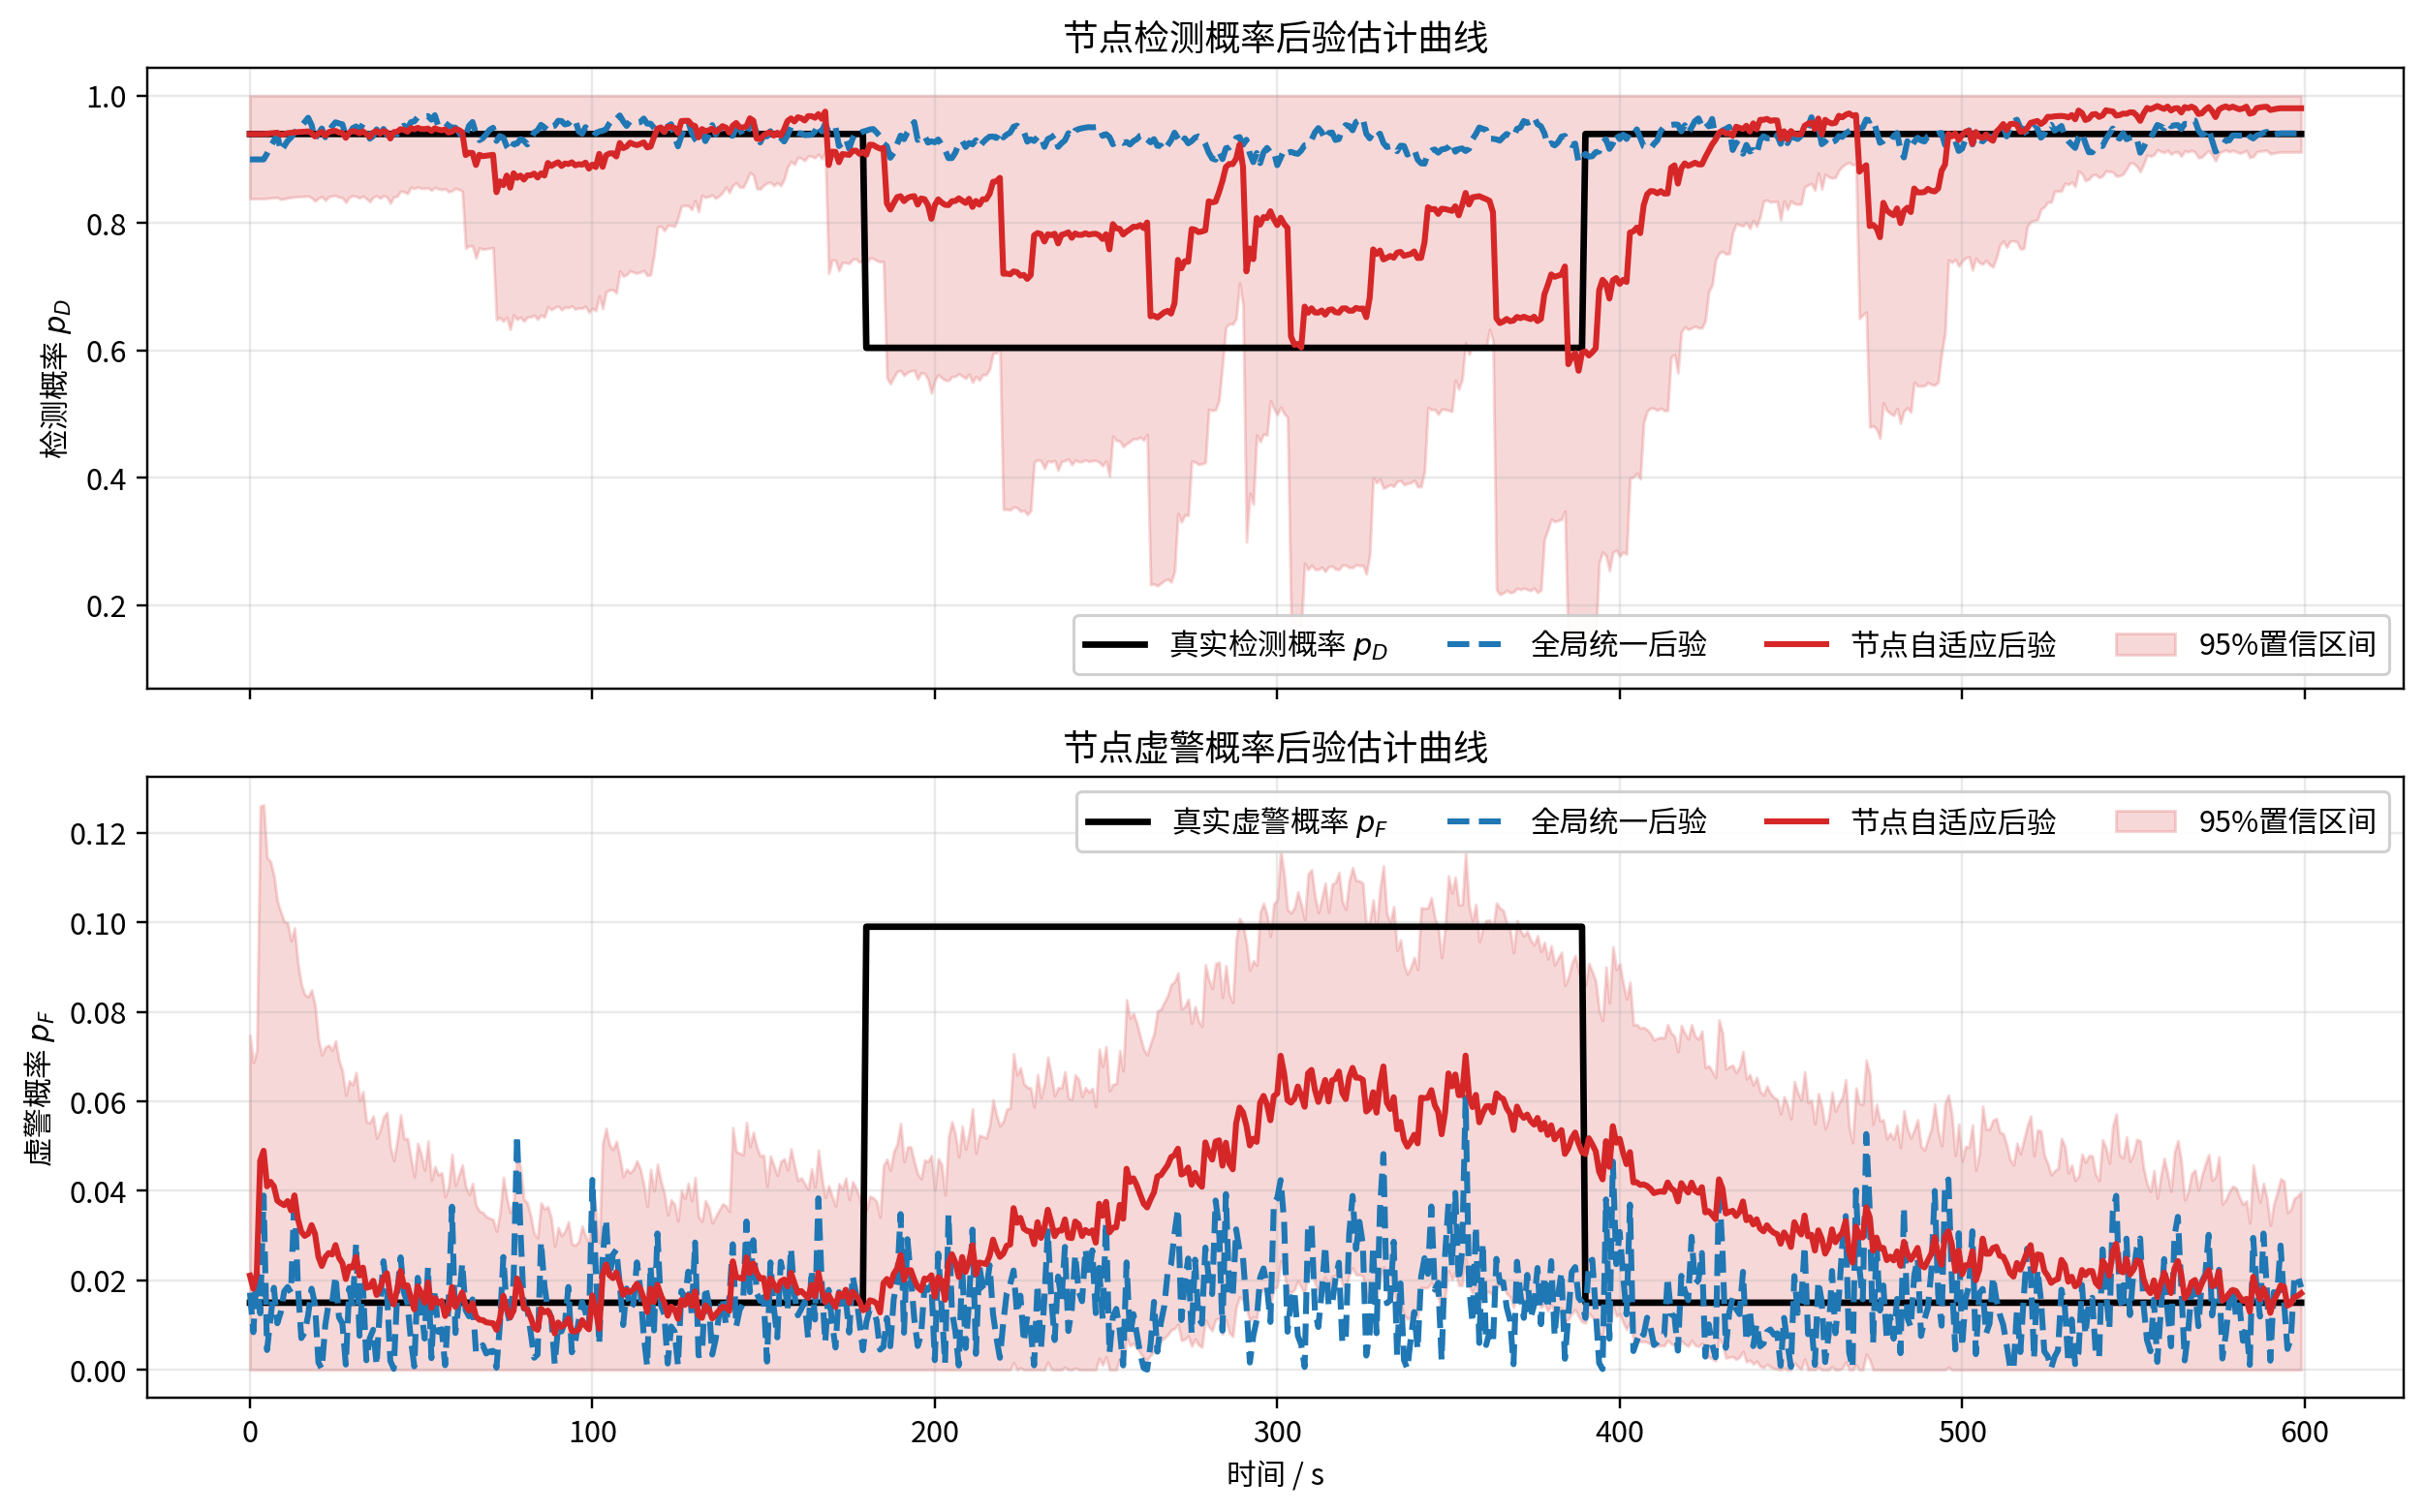
\includegraphics[width=0.88\textwidth]{code/chapter3/experiment1/exp1_results/exp1_node_posterior_curve_v1.png}
	\caption{代表性退化节点的检测概率与杂波强度后验估计曲线}
	\label{fig:ch3_exp2_node_posterior}
\end{figure}

从图~\ref{fig:ch3_exp2_node_posterior} 可以看出，当节点进入退化区间后，本文采用的扫描冻结、软计数累积和窗口定稿后更新策略能够较快跟随真实检测概率的下降趋势，并在退化结束后重新收敛到稳定高值。相比之下，全局统一后验对局部退化的响应存在明显滞后，难以准确刻画单节点性能突变。对于杂波强度，自适应后验能够在退化区间内持续抬升，并在恢复阶段逐步回落，说明该机制能够同时感知漏检增多和误触发增多两类退化现象。

图~\ref{fig:ch3_exp2_degradation_impact} 给出了不同退化强度下的跟踪性能变化。

\begin{figure}[H]
	\centering
	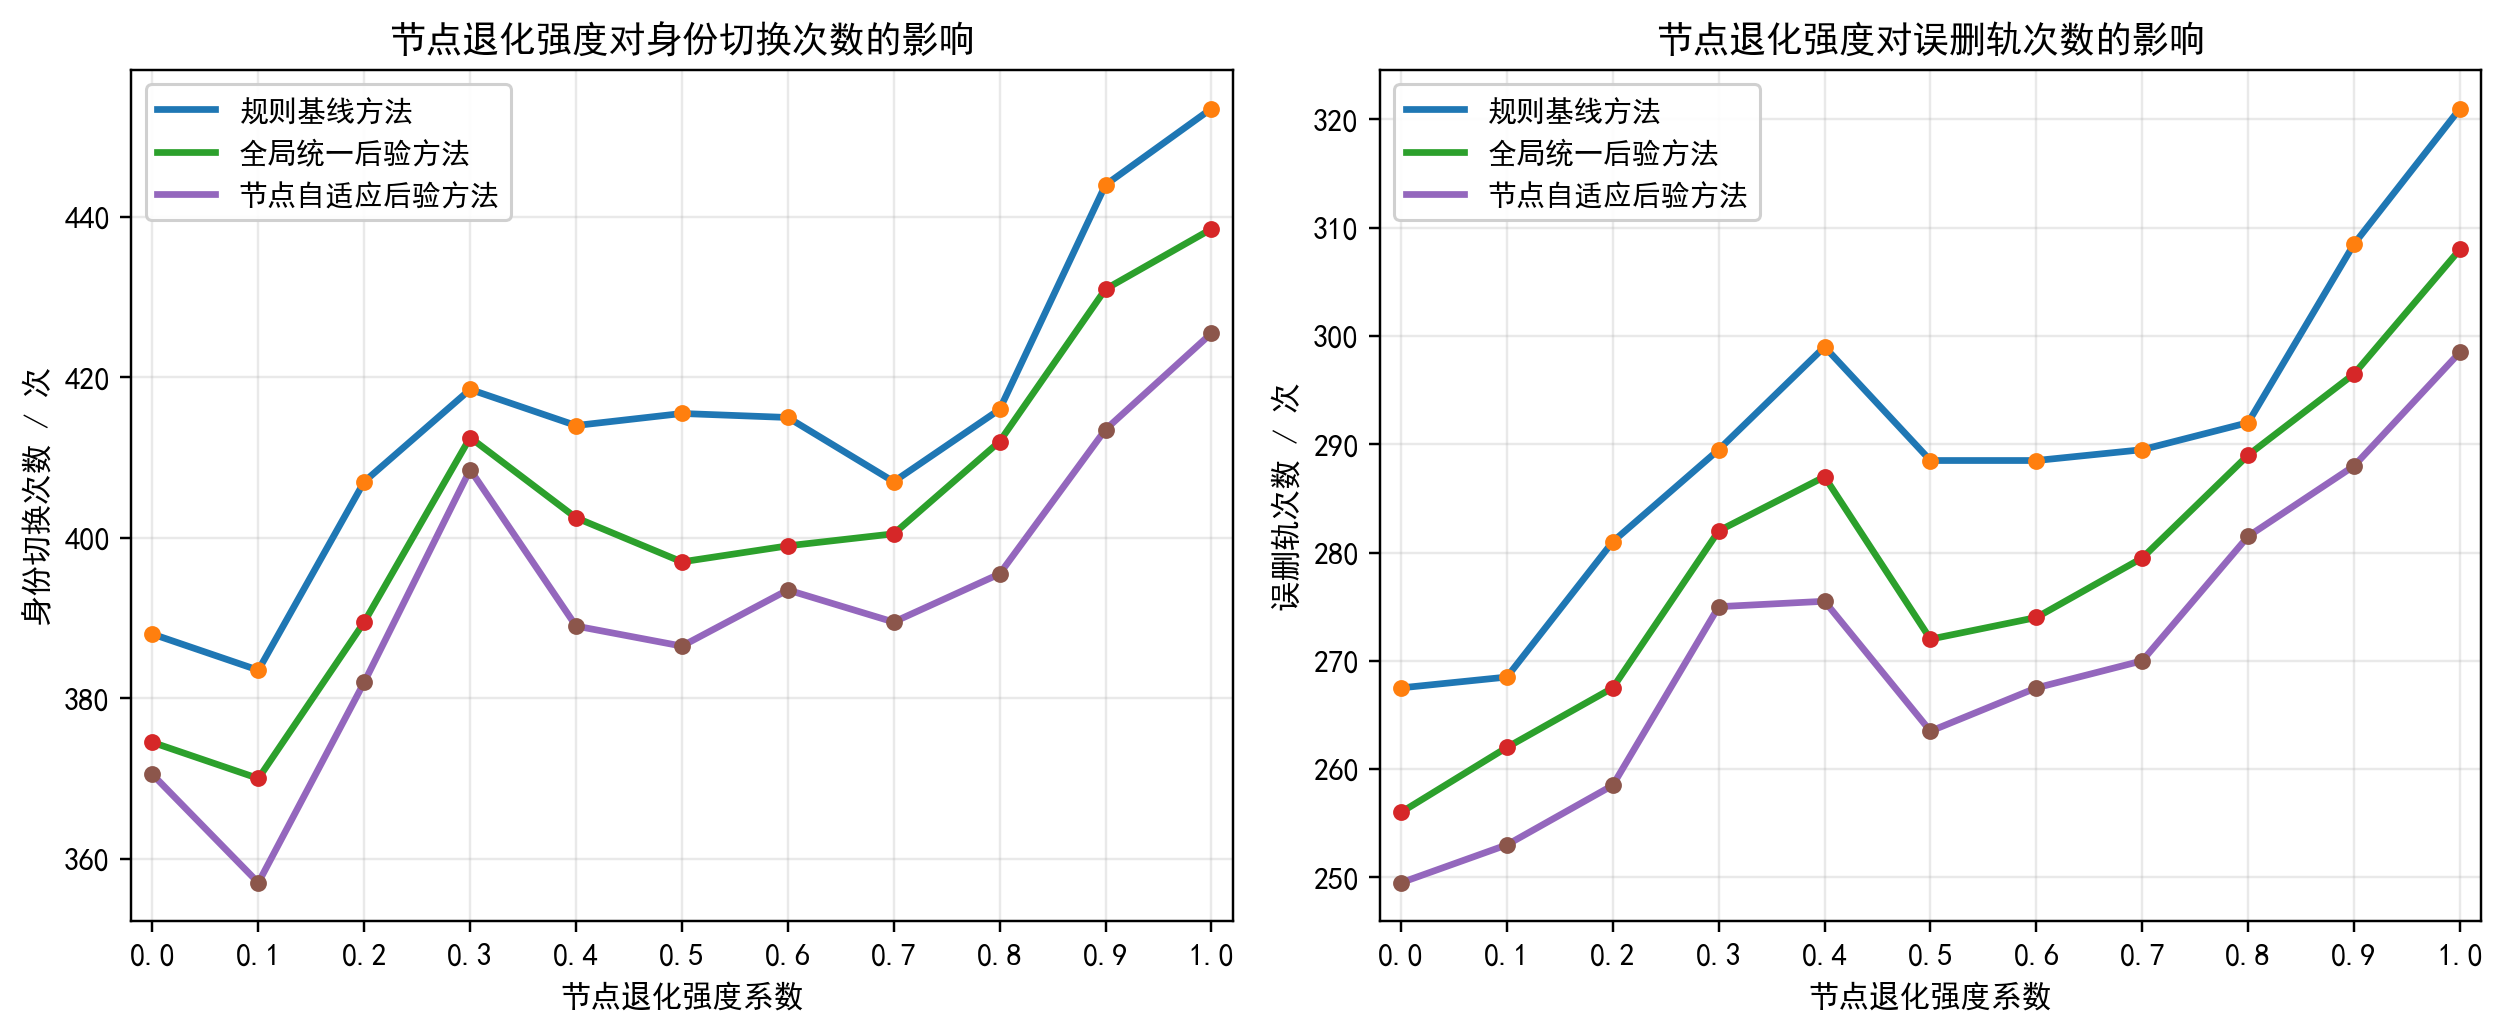
\includegraphics[width=0.88\textwidth]{code/chapter3/experiment1/exp1_results/exp1_degradation_impact_v2.png}
	\caption{节点退化强度对身份切换次数与误删轨迹次数的影响}
	\label{fig:ch3_exp2_degradation_impact}
\end{figure}

随着节点退化强度逐步增加，各方法的身份切换次数和误删轨迹次数均有所上升，但本文方法在整个退化区间内始终保持最低水平。这表明节点后验不仅提高了参数辨识精度，而且通过将节点可靠性显式引入门控与关联过程，实质性降低了节点退化对轨迹连续性和身份一致性的破坏。综合图~\ref{fig:ch3_exp2_node_posterior} 与图~\ref{fig:ch3_exp2_degradation_impact} 可知，节点状态自适应是本章在线跟踪框架成立的重要基础，也为后续场景判别和漏检容忍提供了更可信的先验信息。

\subsection{邻道干扰、双车并行和车道状态更新仿真结果}

\noindent （1）仿真数据生成与参数设置。

邻道干扰与真实双车并行是双车道地磁事件流中最容易混淆的两类场景，也是原有单帧阈值规则最容易失效的部分。为此，本文构造三类典型序列，分别对应单车正常通过、单车通过并伴随邻道干扰，以及两车长时间并行通过。对于困难场景，将两车的初始纵向间隔和速度差压缩在较小范围内，使其在连续多个节点对上保持近似并行，并有意将两车相对时间差长期控制在经验阈值附近，以突出单帧证据不足而多步证据递推有效这一差异。此外，在部分样本中以小概率注入换道行为，使车道后验能够在固定滞后窗口内完成平滑翻转，用于验证场景后验显式进入车道状态递推后的稳定性。

\noindent （2）仿真结果分析。

图~\ref{fig:ch3_exp3_hard_case} 给出了困难双车并行场景下的场景后验递推过程。

\begin{figure}[H]
	\centering
	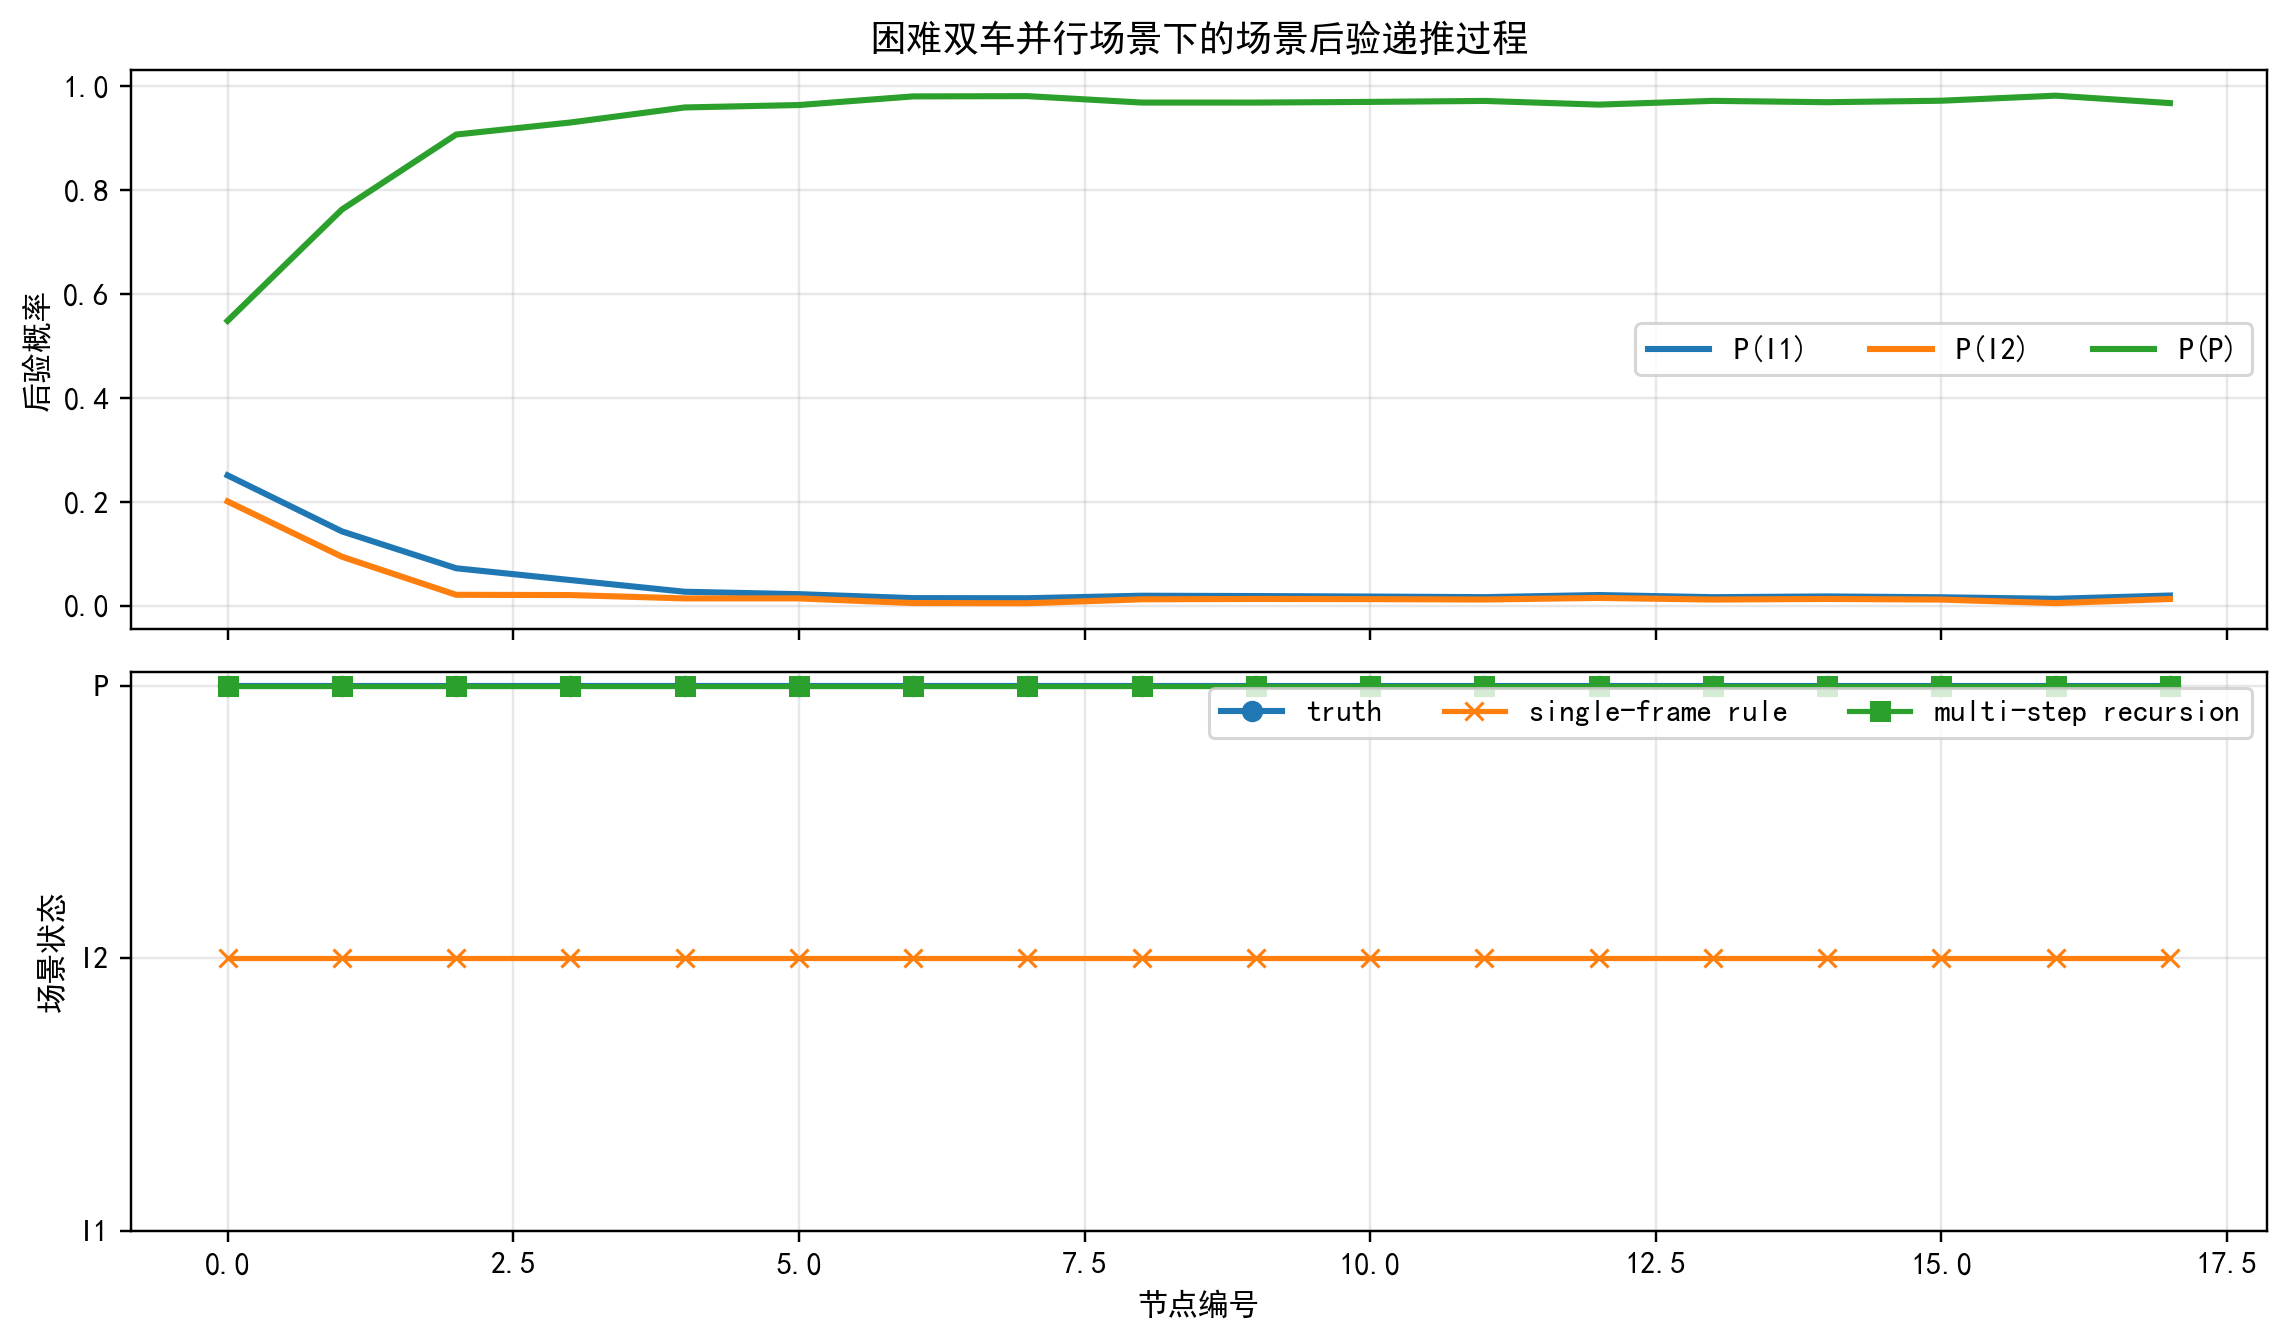
\includegraphics[width=0.88\textwidth]{code/chapter3/experiment3/chapter3_exp345_results/exp3_hard_case_posterior.png}
	\caption{困难双车并行场景下的场景后验递推过程}
	\label{fig:ch3_exp3_hard_case}
\end{figure}

可以看到，单帧阈值规则在整个节点序列上几乎始终停留在邻道干扰状态，未能恢复真实并行关系；而三状态场景递推模型在早期若干节点后便逐步累积并行证据，使并行状态后验持续升高并保持稳定。该结果说明，当相对时间差持续较小、磁峰值差异又不足以单独支撑硬判决时，单帧阈值规则会持续将真实双车并行误判为邻道干扰，而引入状态持续性和多步递推后，这一失效模式能够被显著缓解。

图~\ref{fig:ch3_exp3_metrics} 汇总了实验三的整体指标。

\begin{figure}[H]
	\centering
	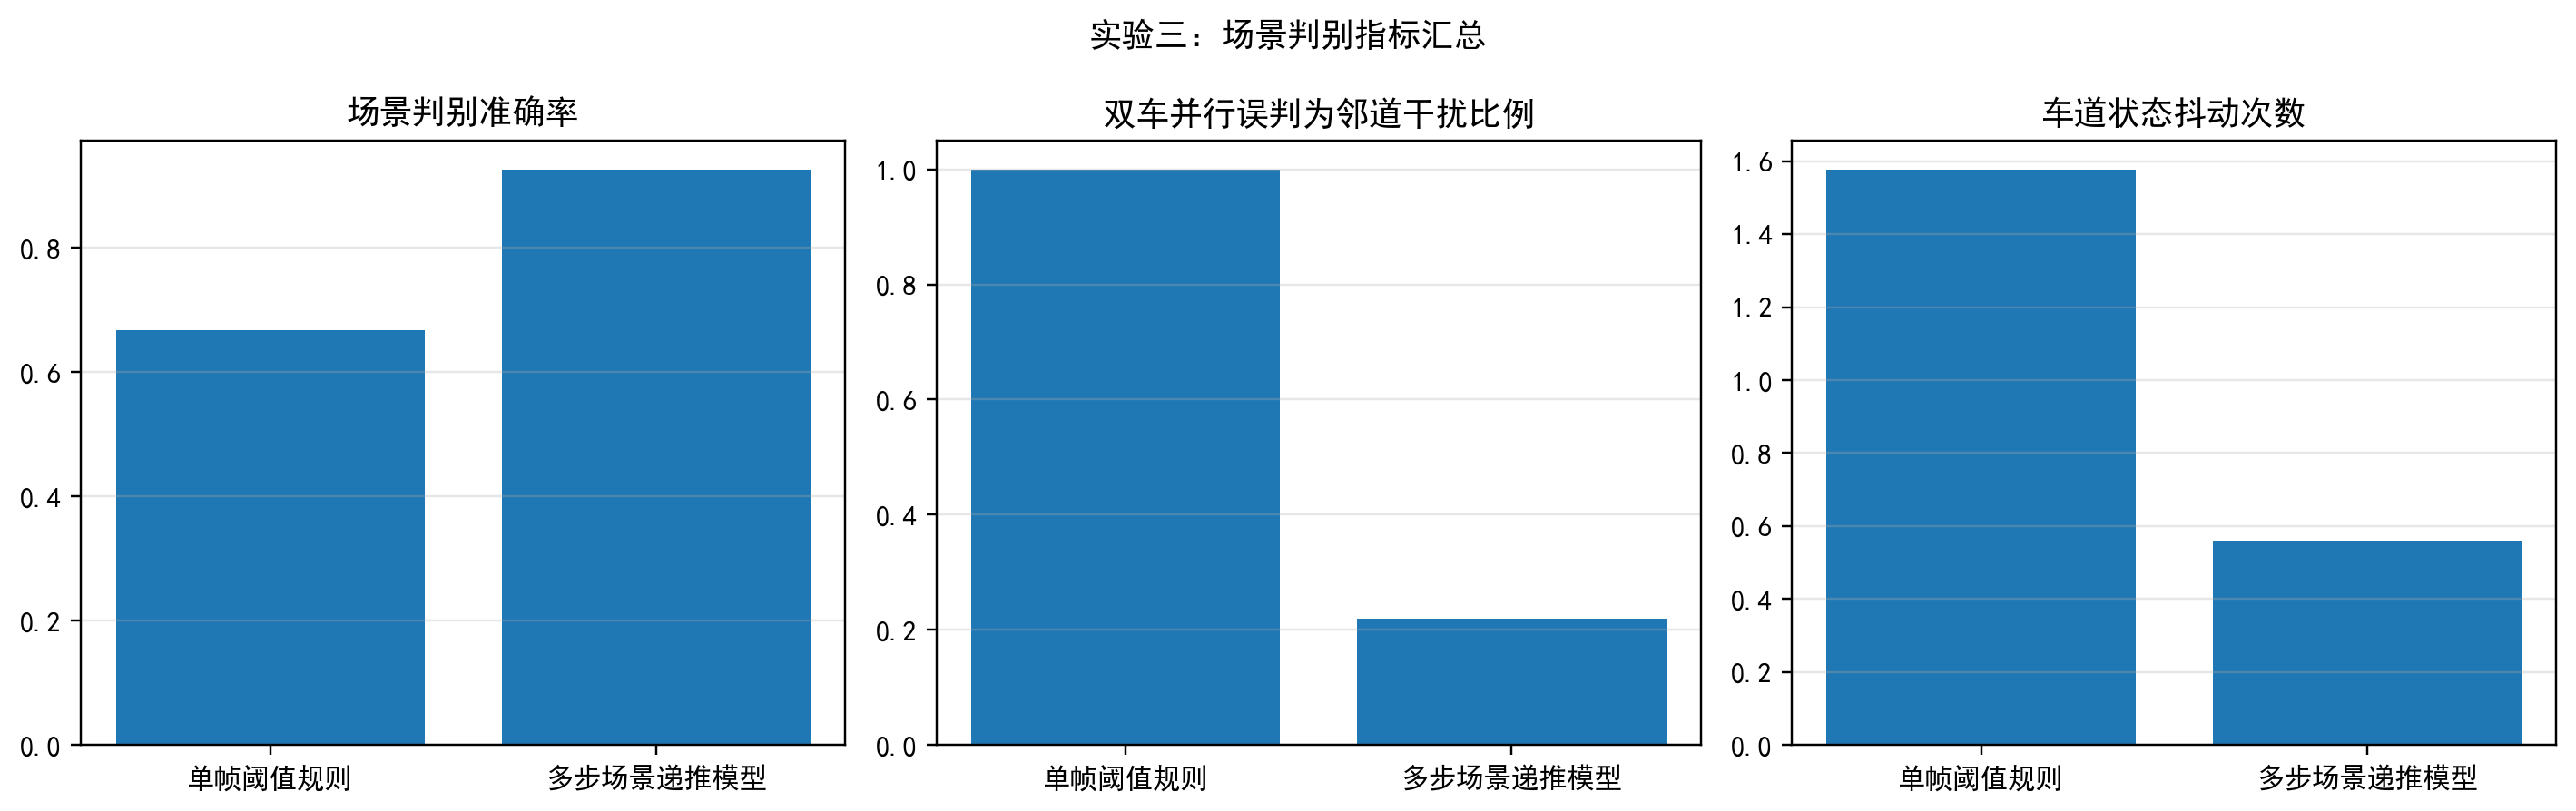
\includegraphics[width=0.92\textwidth]{code/chapter3/experiment3/chapter3_exp345_results/exp3_scene_metrics.png}
	\caption{实验三场景判别与车道状态指标汇总}
	\label{fig:ch3_exp3_metrics}
\end{figure}

结果表明，场景判别准确率由单帧阈值规则的 $0.6667$ 提升至多步场景递推模型的 $0.9262$，车道状态准确率也由 $0.6667$ 提升至 $0.9262$；真实双车并行被误判为邻道干扰的比例由 $1.0000$ 显著下降至 $0.2194$，车道状态抖动次数由 $1.5778$ 下降至 $0.5611$。这说明本文方法的改进并非依赖简单的阈值重整，而是通过三状态场景后验递推完成了对原有失效场景的有效修正。此外，在注入换道动作的扩展样本中，场景后验进入车道状态递推后，车道后验能够在固定滞后窗口内完成由旧车道到新车道的平滑翻转，而不会因单次对侧弱触发产生误切换，这与图~\ref{fig:ch3_exp3_metrics} 中车道状态抖动次数显著下降的结论是一致的。

\subsection{连续漏检容忍范围仿真结果}

\noindent （1）仿真数据生成与参数设置。

在高速路侧部署条件下，短时漏检和短连漏检不可避免。对于第三章方法而言，更重要的问题并不是在理想无漏检条件下是否能够获得最小误差，而是在多大程度上能够维持轨迹连续性和身份一致性。因此，本节在表~\ref{tab:ch3_sim_global} 和表~\ref{tab:ch3_scene_inject} 的基础上，分别在常规车流和低密度车流条件下设置连续漏检长度 $m\in\{1,2,3,4,5\}$，统计轨迹连续保持率、跨段位置均方根误差、身份切换次数和轨迹碎片数的变化趋势，用于确定所提方法对连续漏检的稳定容忍区间。

\noindent （2）仿真结果分析。

图~\ref{fig:ch3_exp4_miss} 给出了不同连续漏检长度下的轨迹连续保持率与跨段位置均方根误差。

\begin{figure}[H]
	\centering
	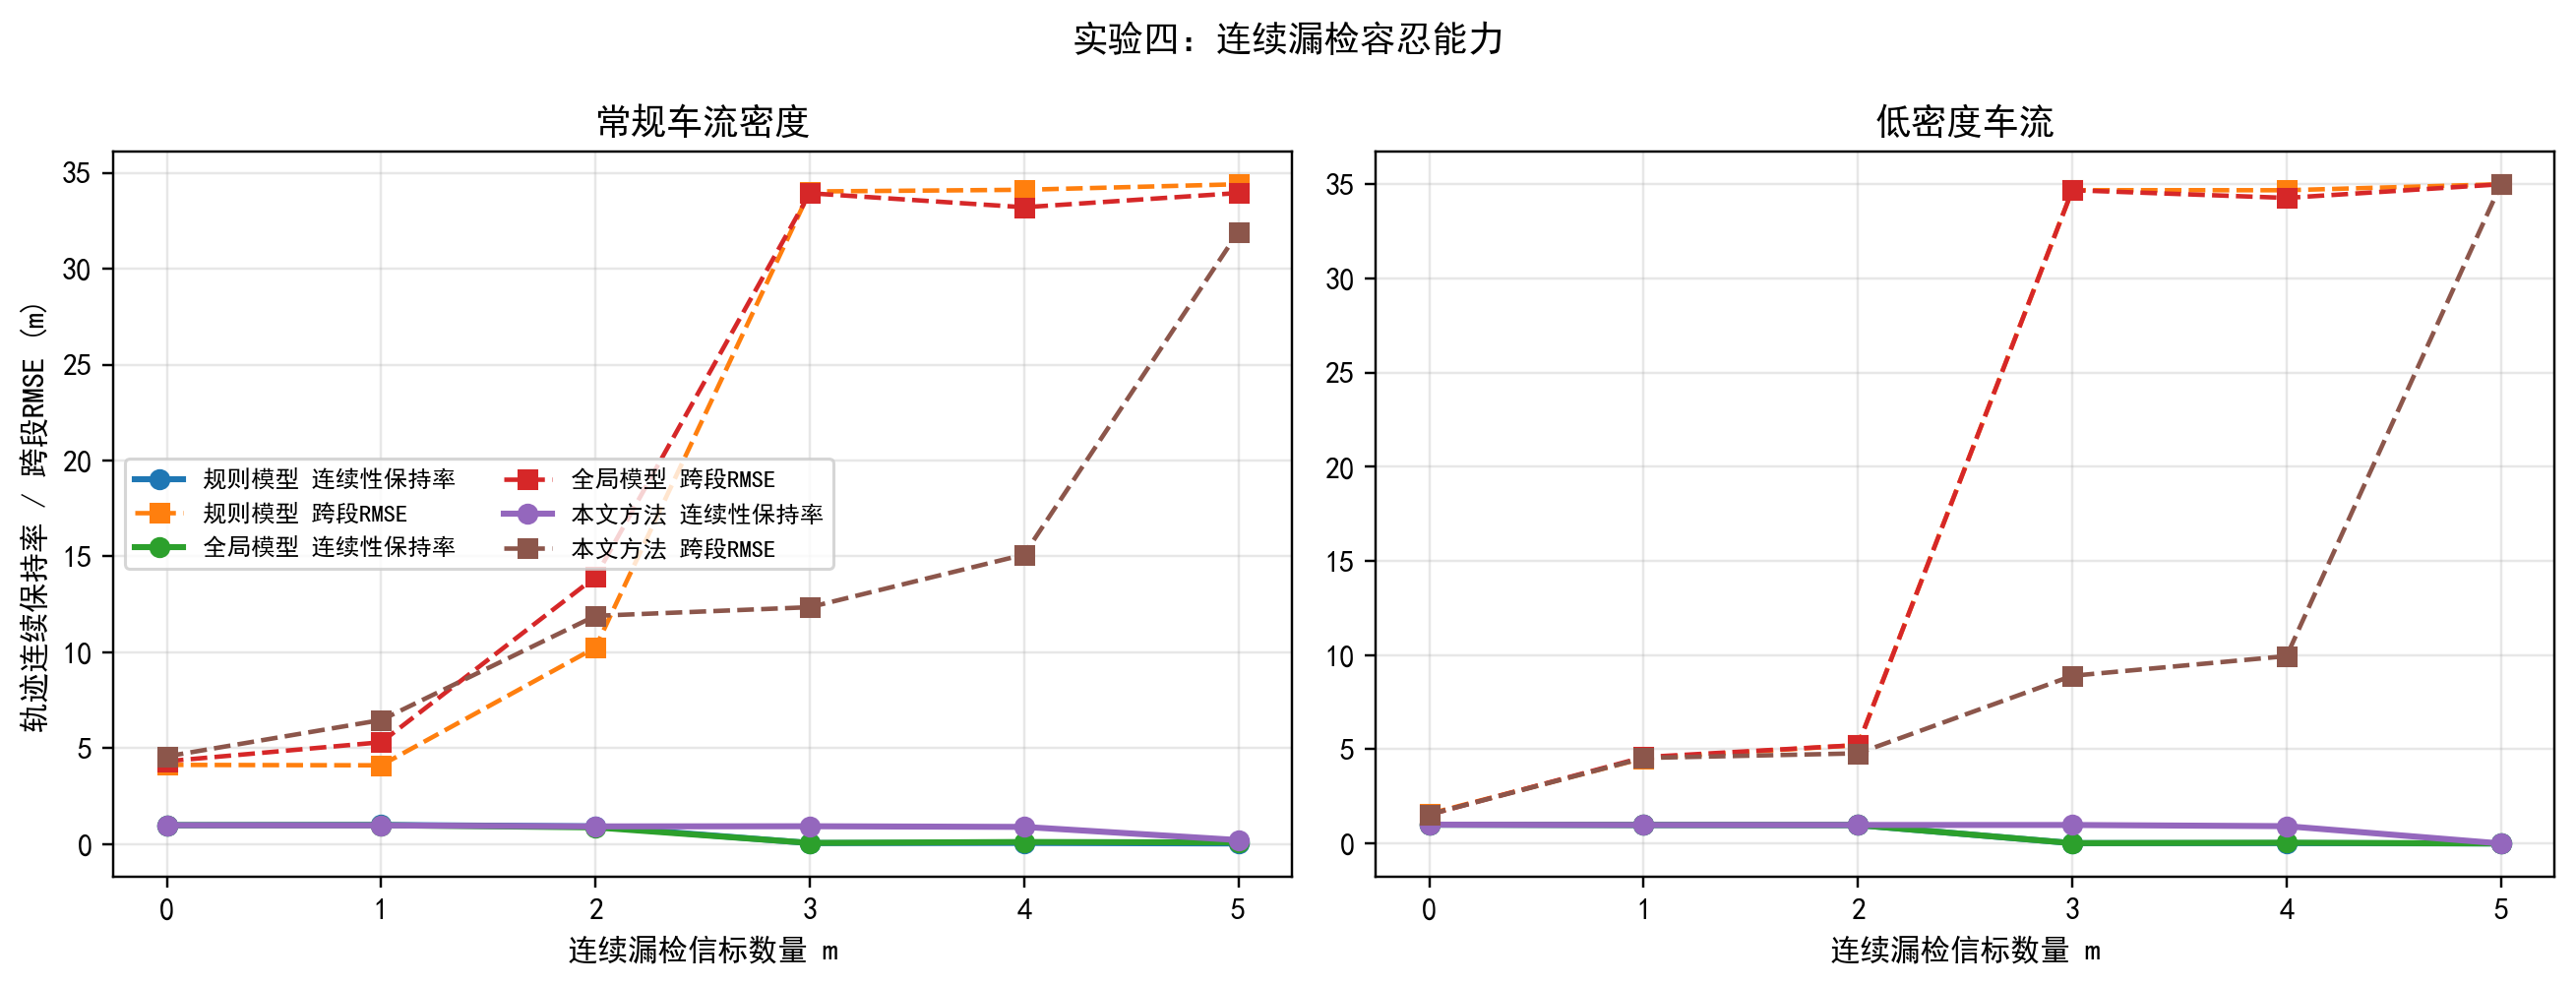
\includegraphics[width=0.95\textwidth]{code/chapter3/experiment3/chapter3_exp345_results/exp4_miss_tolerance.png}
	\caption{不同连续漏检长度下的轨迹连续保持率与跨段 RMSE}
	\label{fig:ch3_exp4_miss}
\end{figure}

由图~\ref{fig:ch3_exp4_miss} 可见，本文方法在常规车流条件下对连续 2 至 3 个节点漏检仍保持较稳定的轨迹连续性。当 $m=2,3,4$ 时，轨迹连续保持率分别为 $0.9233$、$0.9321$ 和 $0.8981$，对应跨段位置均方根误差分别为 $11.90\ \mathrm{m}$、$12.35\ \mathrm{m}$ 和 $15.10\ \mathrm{m}$。在低密度车流条件下，该容忍范围可进一步扩展。当 $m=2,3,4$ 时，轨迹连续保持率分别为 $0.9821$、$0.9821$ 和 $0.9188$，对应跨段位置均方根误差分别为 $4.78\ \mathrm{m}$、$8.90\ \mathrm{m}$ 和 $9.95\ \mathrm{m}$。

上述结果说明，第三章方法的稳定容忍区间主要集中在常规车流下的连续 2 至 3 个节点，以及低密度条件下的连续 3 至 4 个节点。一旦超过该范围，门控范围扩张和身份歧义会共同导致轨迹碎片化明显加重。从章节衔接角度看，该实验也为第四章的研究定位提供了直接依据。由于第三章方法已经能够在在线条件下处理短时漏检和短连漏检问题，因此第四章更适合作为其下游片段级重构模块，重点处理超过固定滞后窗口和删除阈值之后形成的长时间间断片段，而不是重复解决第三章已能较好覆盖的短间断情形。

\subsection{时间组织与固定滞后回放仿真结果}

\noindent （1）仿真数据生成与参数设置。

本节用于验证扫描化处理、事件驱动更新和固定滞后回放相结合的时间组织方式是否合理。实验以实测延迟分布为约束，对事件到达顺序进行随机扰动，并分别扫描时间片长度 $\Delta T$ 和固定滞后窗口长度 $L$。在每组配置下，统计同一扫描内相邻节点的同车触发比例、迟到量测吸收比例，以及在线回放结果与按触发时间离线重排结果之间的一致率，用于考察时间组织参数对在线结果稳定性的影响。

\noindent （2）仿真结果分析。

图~\ref{fig:ch3_exp5_time} 给出了实验五的三类统计结果。

\begin{figure}[H]
	\centering
	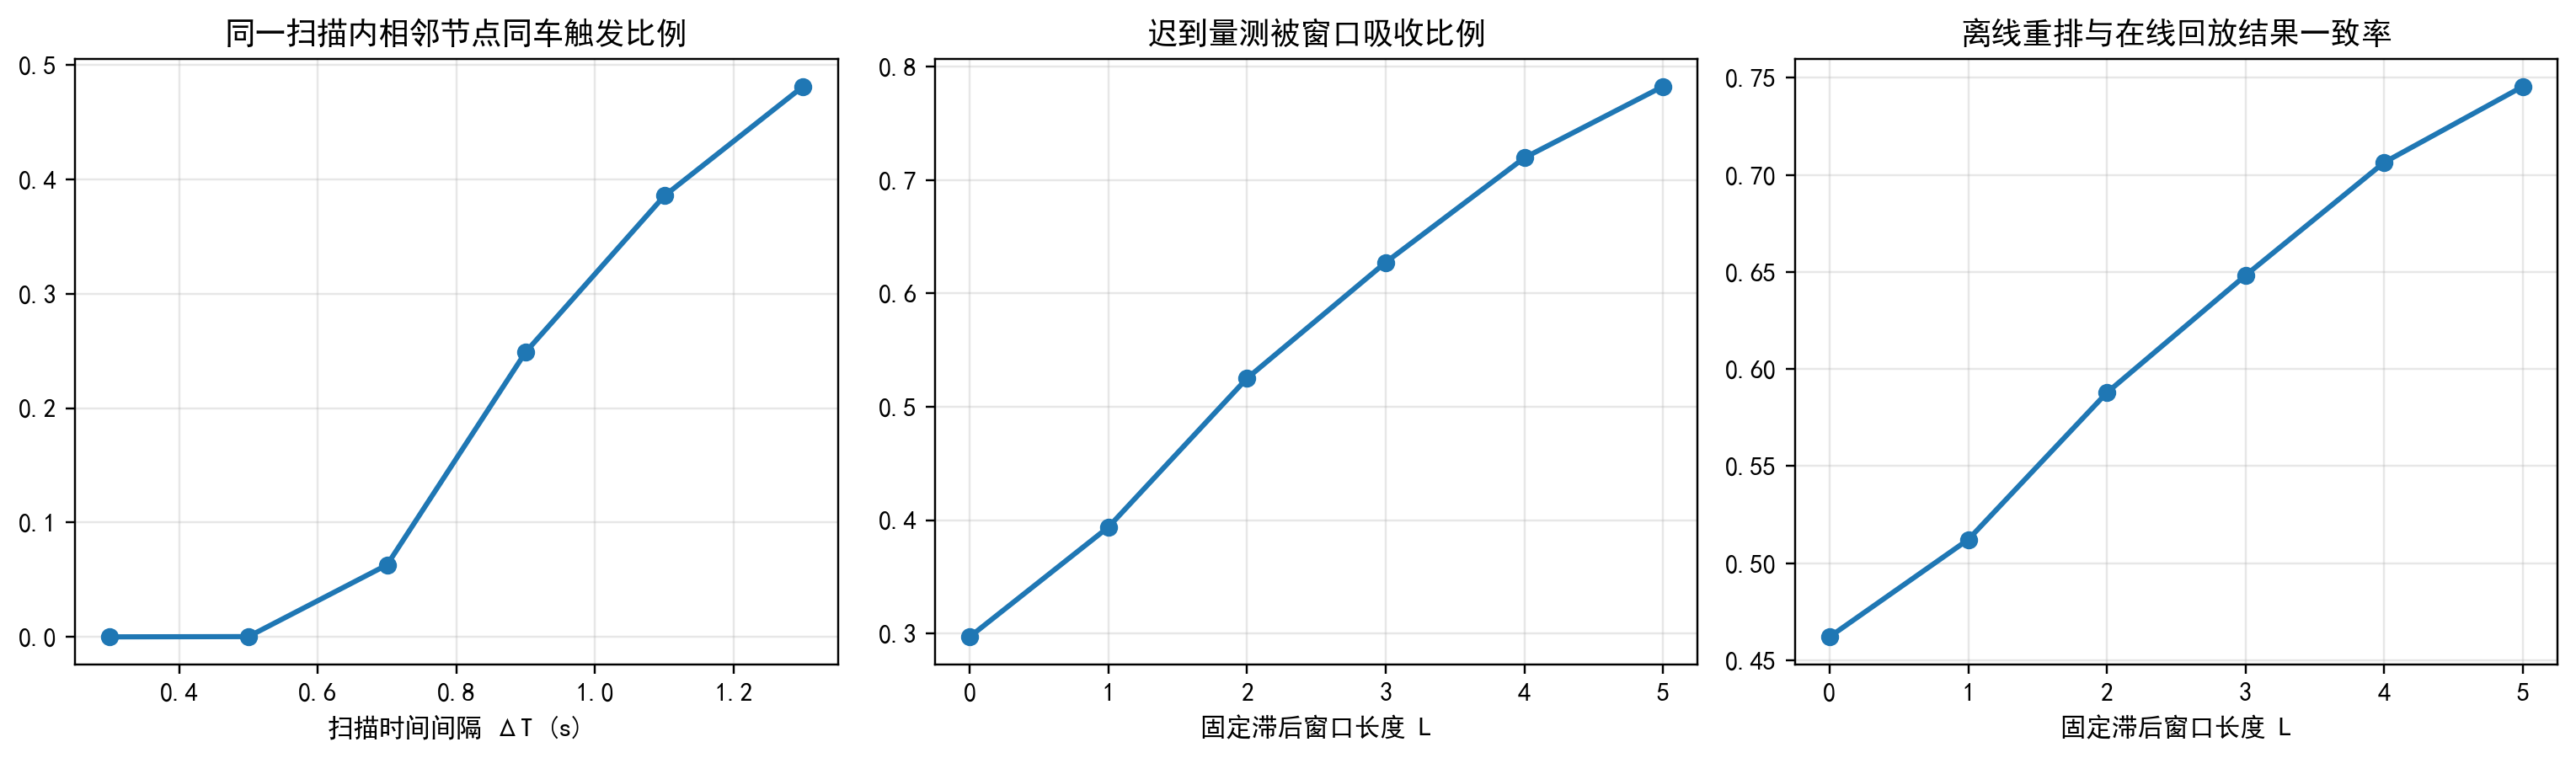
\includegraphics[width=0.95\textwidth]{code/chapter3/experiment3/chapter3_exp345_results/exp5_time_consistency.png}
	\caption{时间组织与固定滞后回放一致性实验结果}
	\label{fig:ch3_exp5_time}
\end{figure}

首先，随着 $\Delta T$ 增大，同一扫描内相邻节点同车触发比例单调提升，说明过小的扫描间隔会削弱扫描组织对相邻节点事件的吸纳能力，而适度增大 $\Delta T$ 有利于提升局部时间组织的一致性。其次，迟到量测被窗口吸收的比例随 $L$ 增大而持续上升。当 $L=0,1,2,3,4,5$ 时，吸收比例分别为 $0.2970$、$0.3937$、$0.5250$、$0.6272$、$0.7194$ 和 $0.7824$。再次，离线重排与在线回放结果一致率也随 $L$ 增长而稳步提升，对应取值分别为 $0.4620$、$0.5121$、$0.5878$、$0.6482$、$0.7064$ 和 $0.7456$。这说明固定滞后窗口确实能够在不过度牺牲实时性的前提下吸收迟到量测，并显著改善在线处理与离线最优时间顺序之间的一致性。

综合图中结果可见，当 $L=4$ 时，迟到量测吸收比例达到 $0.7194$，在线与离线结果一致率达到 $0.7064$，已经能够在精度收益和额外开销之间取得较好的折中。因此，除时间组织扫描实验外，本文后续实验统一取 $L=4$ 作为默认配置。

\subsection{消融实验与复杂度分析}

\noindent （1）消融设置。

为验证本章方法不是对原有规则的局部修补，而是由若干可解释模块共同构成的统一概率递推模型，本节从场景判别、跟踪连续性和时间回放三个角度分别进行定向消融，并进一步分析固定滞后窗口长度对额外开销的影响。具体消融项包括去除三状态场景递推、去除节点状态自适应、去除磁特征一致性、将软计数定稿更新替换为当前扫描的硬计数即时更新，以及去除固定滞后回放模块。

\noindent （2）消融结果分析。

图~\ref{fig:ch3_ablation_scene} 给出了场景递推模块的定向消融结果。

\begin{figure}[H]
	\centering
	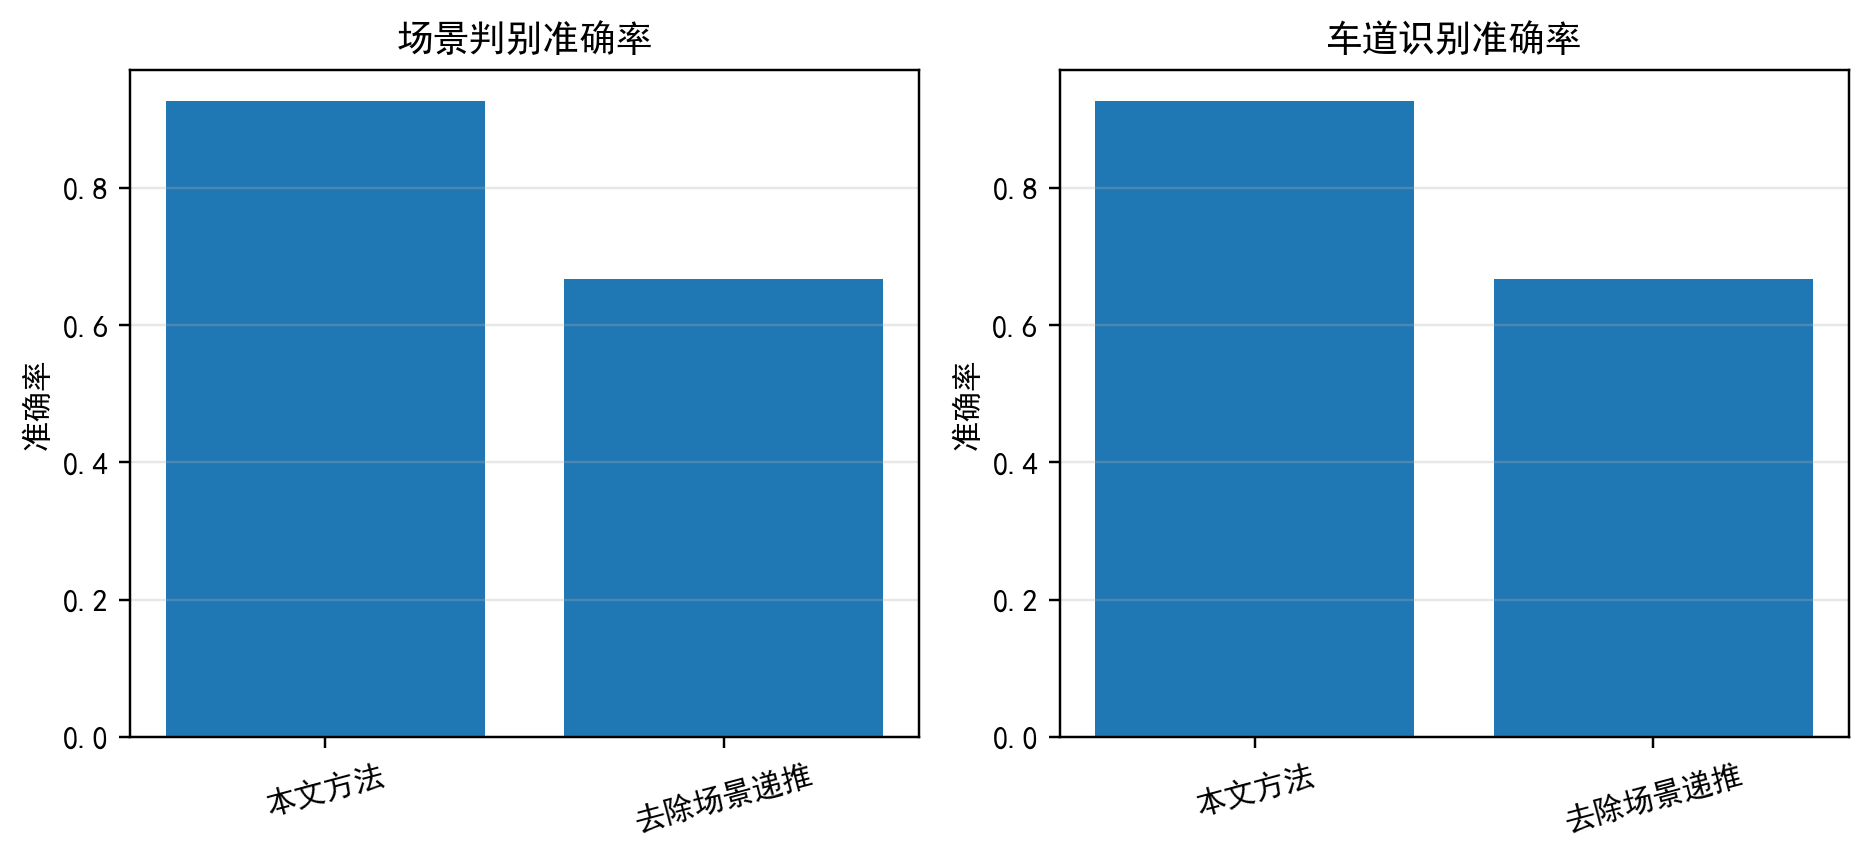
\includegraphics[width=0.75\textwidth]{code/chapter3/experiment3/chapter3_exp345_results/ablation_scene_targeted.png}
	\caption{场景递推模块的定向消融结果}
	\label{fig:ch3_ablation_scene}
\end{figure}

由图~\ref{fig:ch3_ablation_scene} 可见，去掉三状态场景递推，仅保留单帧时间阈值和磁峰值规则后，场景判别准确率和车道识别准确率均由本文方法的 $0.9144$ 下降至 $0.6667$。这说明场景递推并非附属模块，而是支撑双车并行与邻道干扰区分能力的核心组成部分。

图~\ref{fig:ch3_ablation_track} 给出了跟踪侧关键模块的定向消融结果。

\begin{figure}[H]
	\centering
	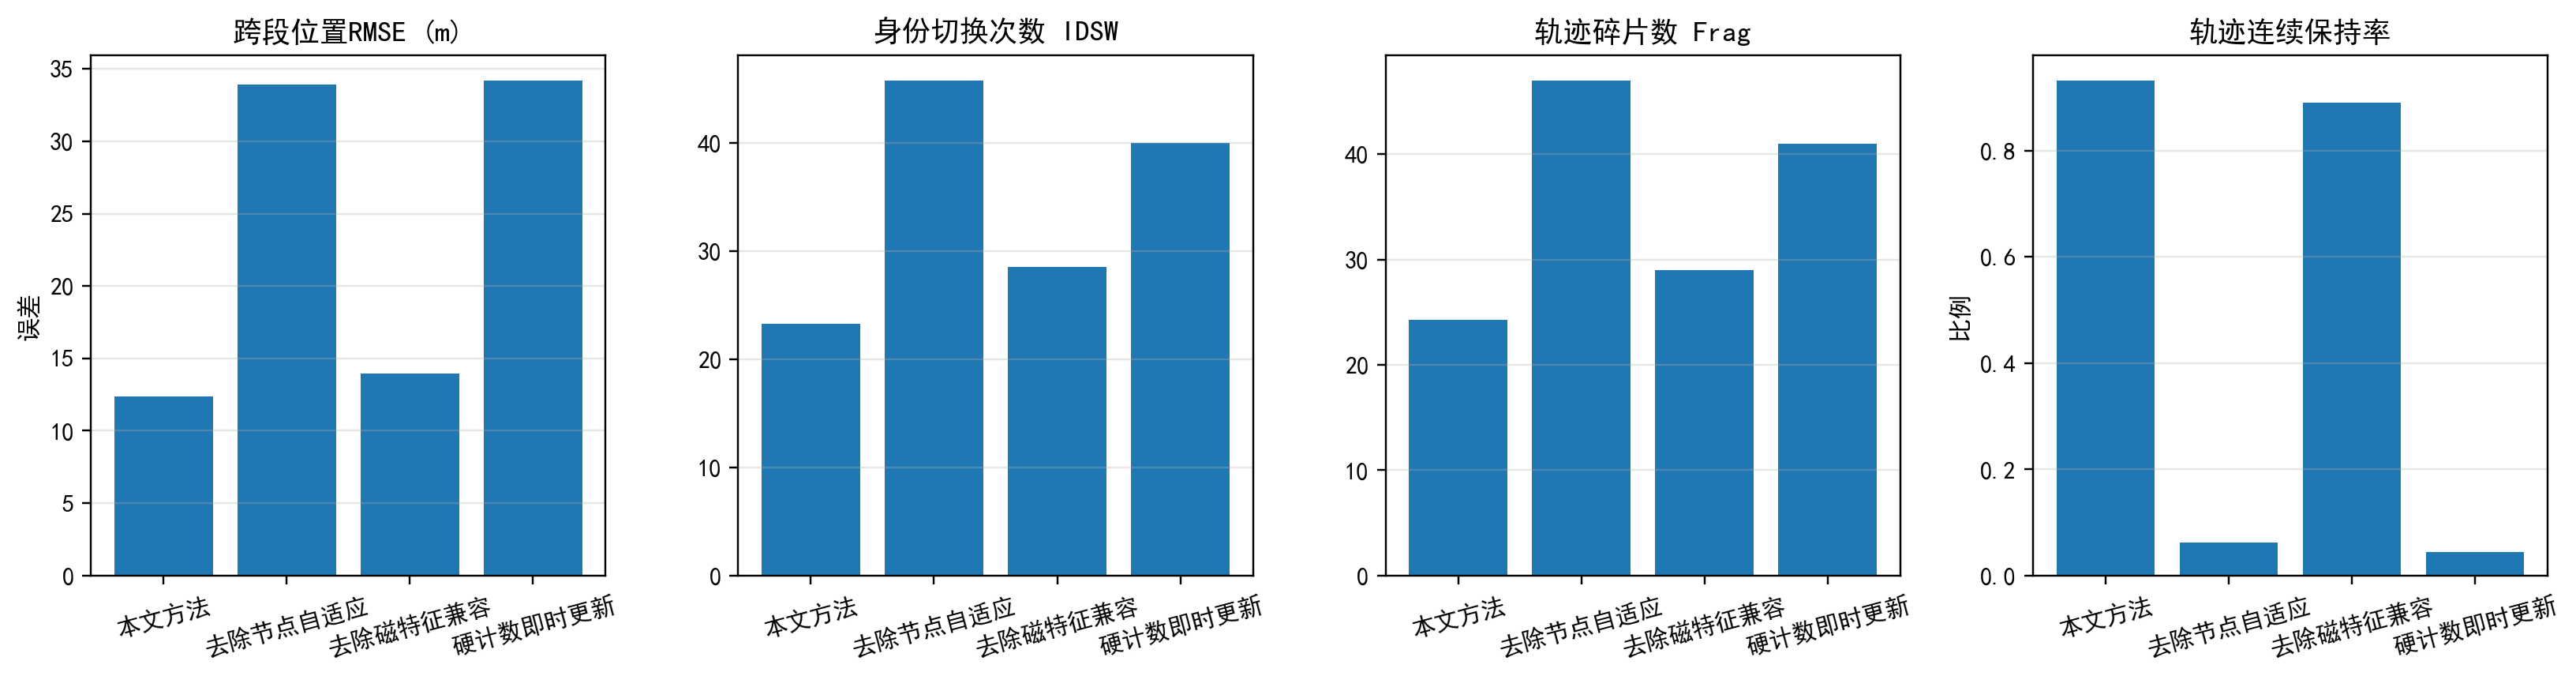
\includegraphics[width=0.95\textwidth]{code/chapter3/experiment3/chapter3_exp345_results/ablation_tracking_targeted.png}
	\caption{跟踪侧关键模块的定向消融结果}
	\label{fig:ch3_ablation_track}
\end{figure}

可以看到，去掉节点状态自适应后，跨段位置均方根误差和轨迹连续保持率均有所恶化；将软计数定稿更新替换为硬计数即时更新后，桥接位置均方根误差急剧上升，轨迹连续保持率显著下降，说明该模块对于抑制错误自强化、维持短连漏检条件下的轨迹连续性具有关键作用。相比之下，仅去掉磁特征一致性时，虽然位置误差、身份切换次数和轨迹碎片数均出现一定退化，但下降幅度明显小于硬计数即时更新的情形，说明磁特征主要在候选冲突和相邻目标近距离竞争时提供辅助判别信息。

图~\ref{fig:ch3_ablation_replay} 给出了固定滞后回放模块的定向消融结果。

\begin{figure}[H]
	\centering
	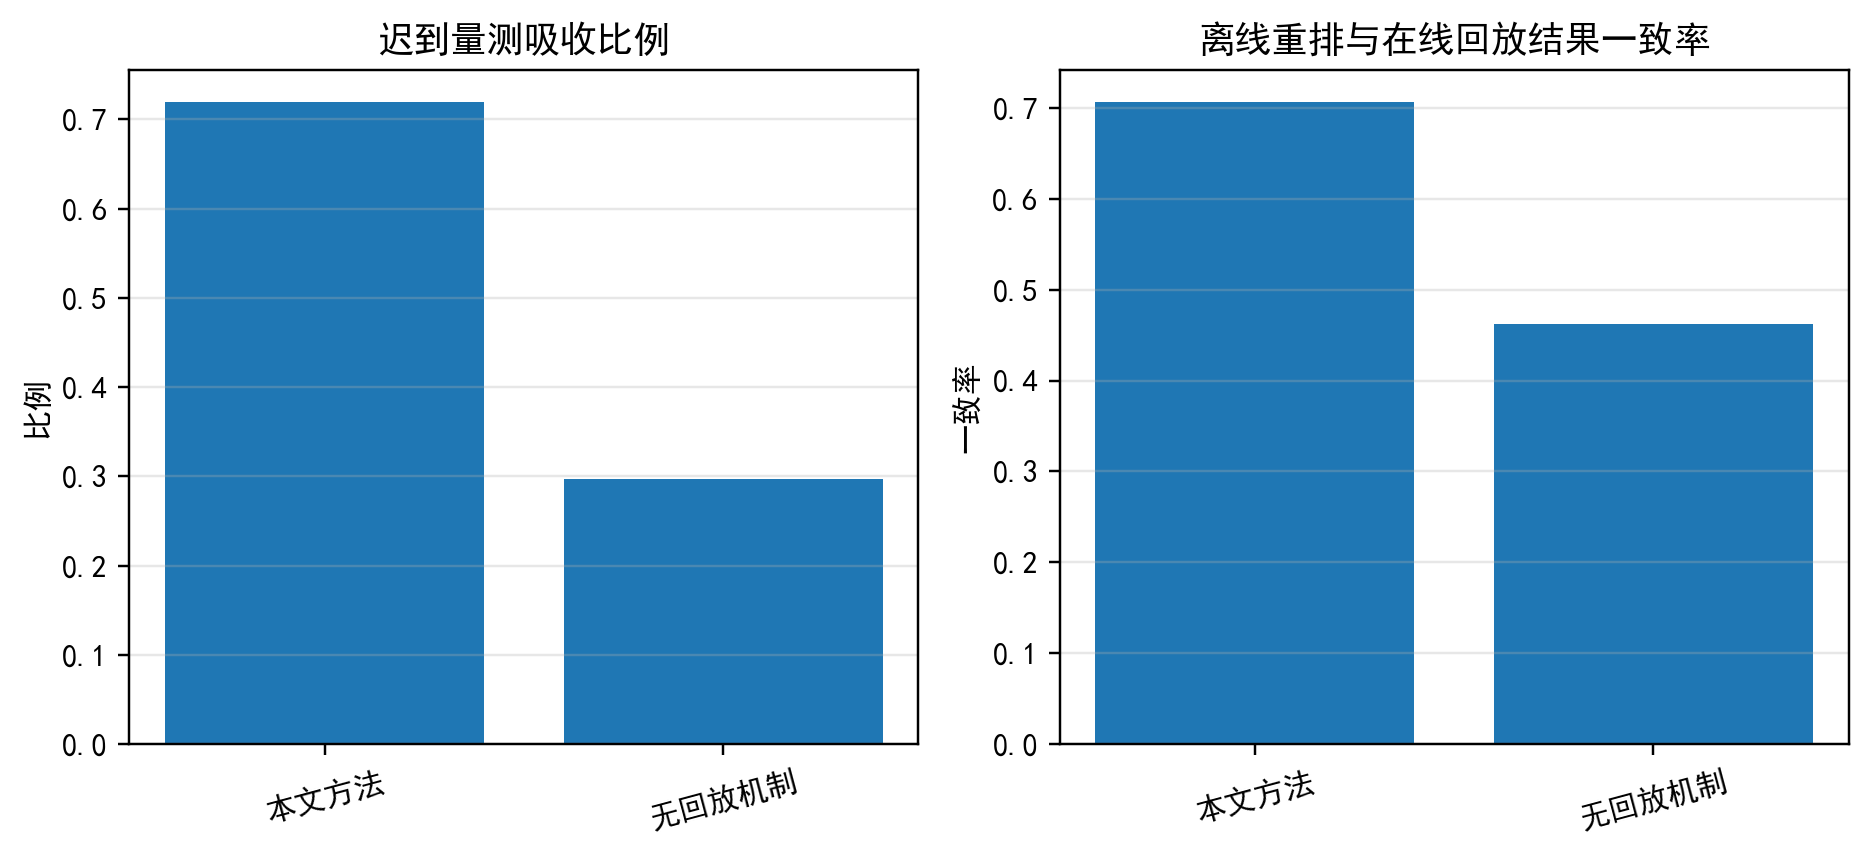
\includegraphics[width=0.75\textwidth]{code/chapter3/experiment3/chapter3_exp345_results/ablation_replay_targeted.png}
	\caption{固定滞后回放模块的定向消融结果}
	\label{fig:ch3_ablation_replay}
\end{figure}

由图~\ref{fig:ch3_ablation_replay} 可见，去掉固定滞后回放后，迟到量测吸收比例由 $0.7194$ 降至 $0.2970$，离线重排与在线回放结果一致率由 $0.7064$ 降至 $0.4620$。这表明回放模块不仅改善了量测时序一致性，而且直接影响在线结果的可复现性，因此其作用应视为本章时间组织模型的一部分，而不是简单的工程性补丁。

图~\ref{fig:ch3_complexity} 给出了固定滞后窗口长度 $L$ 的复杂度与收益折中关系。

\begin{figure}[H]
	\centering
	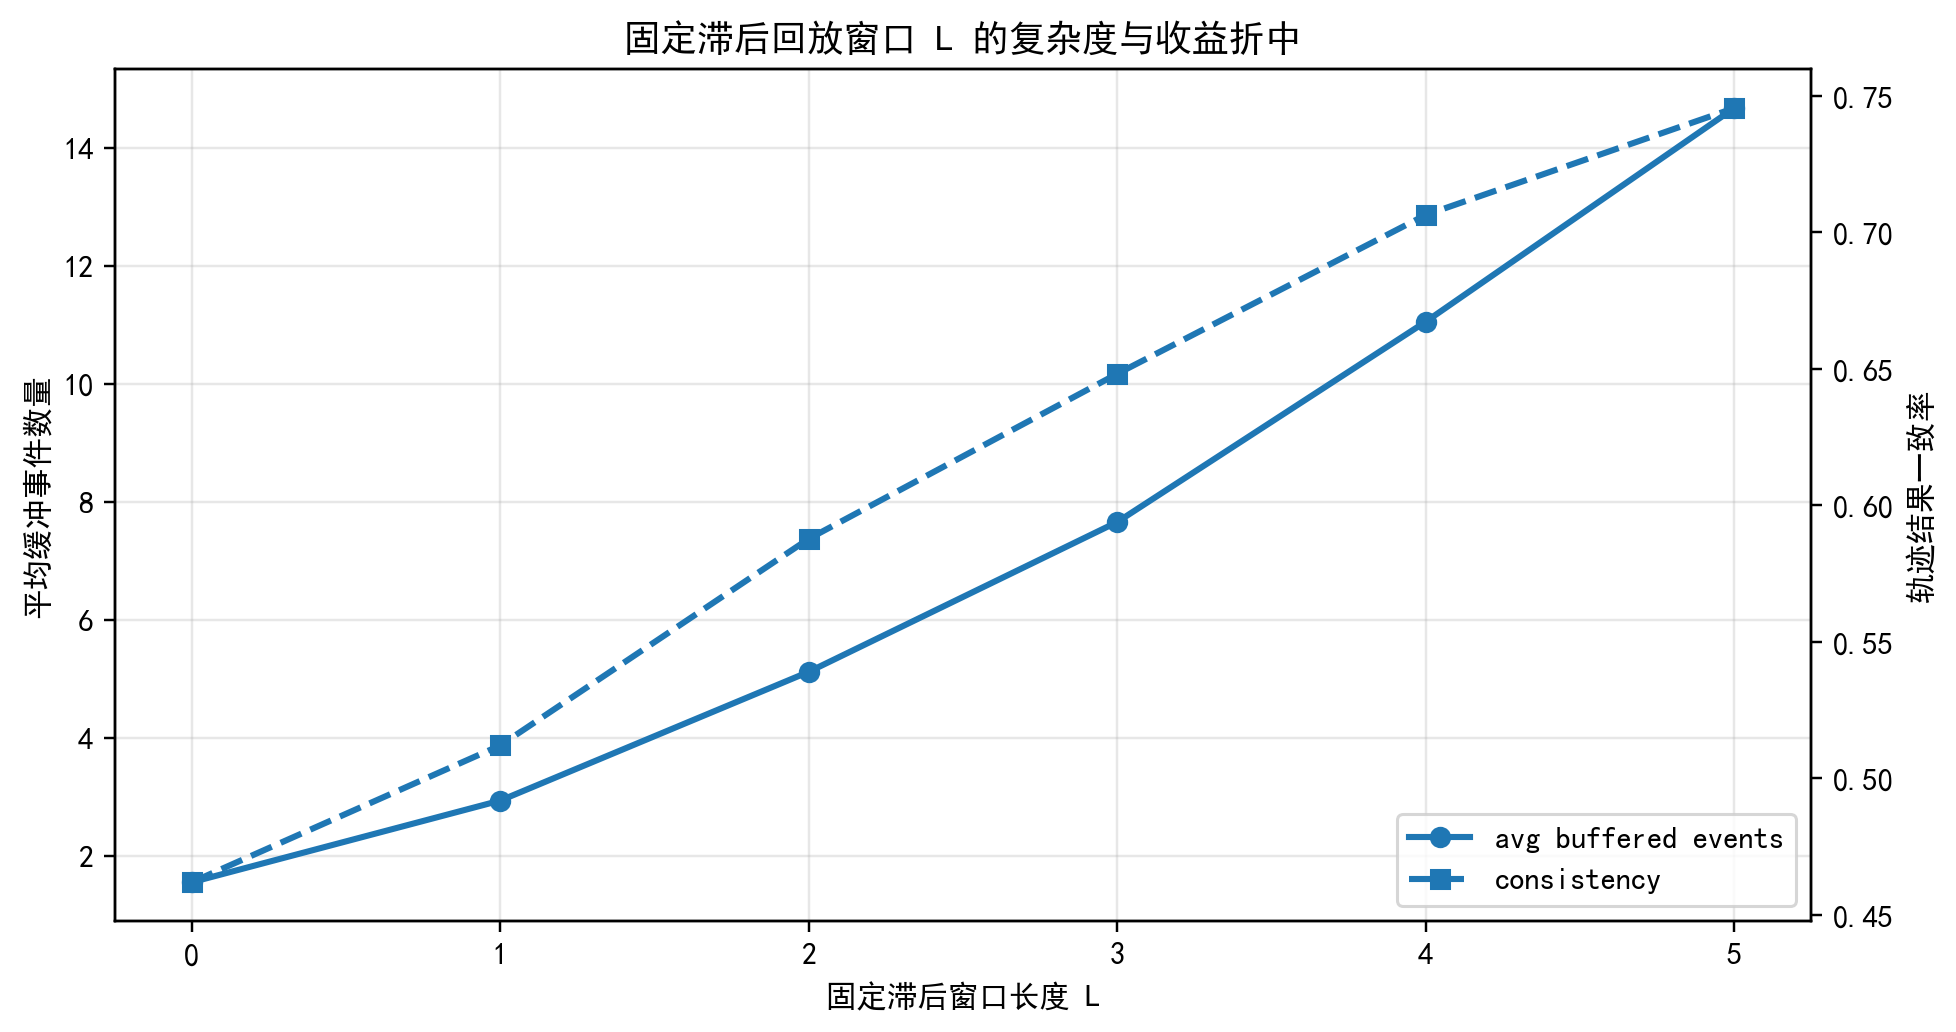
\includegraphics[width=0.78\textwidth]{code/chapter3/experiment3/chapter3_exp345_results/complexity_tradeoff.png}
	\caption{固定滞后窗口长度 $L$ 的复杂度与收益折中关系}
	\label{fig:ch3_complexity}
\end{figure}

随着固定滞后窗口长度 $L$ 增大，平均缓冲事件数由 $1.5517$ 增加到 $14.6682$，说明额外开销与 $L$ 之间呈现近似线性增长关系；与此同时，轨迹结果一致率由 $0.4620$ 提升至 $0.7456$。结合图~\ref{fig:ch3_exp5_time} 与图~\ref{fig:ch3_complexity} 可见，当 $L=4$ 时，迟到量测吸收比例达到 $0.7194$，一致率达到 $0.7064$，而缓冲规模尚处于可接受范围内，因此本文在后续实验中取 $L=4$ 作为精度收益与额外开销之间的折中选择。

\begin{table}[H]
	\centering
	\caption{不同机制对跟踪性能的消融实验结果}
	\label{tab:ablation_tracking}
	\begin{tabular}{lcccc}
		\toprule
		方法 & 桥接位置 RMSE（m） & ID 切换次数 & 轨迹碎片数 & 轨迹保持率 \\
		\midrule
		本文完整方法 & 12.35 & 23.25 & 24.25 & 0.9321 \\
		去除节点状态自适应 & 12.70 & 23.50 & 24.50 & 0.9188 \\
		去除磁特征一致性 & 12.70 & 26.50 & 27.00 & 0.8981 \\
		硬计数即时更新 & 34.21 & 40.00 & 41.00 & 0.0441 \\
		\bottomrule
	\end{tabular}
\end{table}

\subsection{本节小结}

本节围绕节点后验估计能力、邻道干扰与双车并行判别能力、连续漏检容忍范围、时间组织一致性以及各关键模块的独立贡献进行了系统验证。实验结果表明：节点状态自适应后验能够在节点退化与恢复过程中稳定跟踪检测概率和杂波强度变化；三状态场景递推显著降低了真实双车并行被误判为邻道干扰的比例，并有效抑制车道状态抖动；在常规车流条件下，本文方法可较稳定地容忍连续 2 至 3 个节点漏检，在低密度条件下该范围可扩展至连续 3 至 4 个节点；固定滞后回放能够明显提升迟到量测吸收比例以及在线处理结果与离线重排结果的一致率。消融实验进一步说明，节点状态自适应、三状态场景判别、磁特征一致性、软计数定稿更新以及固定滞后回放均对本章方法的最终性能具有独立而明确的贡献。综合来看，上述结果不仅验证了本文方法的精度与鲁棒性，也明确了其适用边界，并为第四章面向长缺测工况的片段级在线聚类与轨迹重构提供了合理的输入条件与触发依据。


\chapter{连续漏检场景下的多地磁传感器车辆轨迹实时聚类算法}
\label{chap:cedas_fragment}

\graphicspath{
	{code/chapter4/experiment123/chapter4_results/exp1/}
	{code/chapter4/experiment123/chapter4_results/exp2/}
	{code/chapter4/experiment123/chapter4_results/exp3/}
}

\section{引言}

第三章主要面向常态工况下的在线车辆目标跟踪问题，通过事件级关联、状态估计与轨迹管理实现了车辆轨迹的持续更新。在短时漏检条件下，上游跟踪器仍可以依靠局部时序信息和在线关联结果维持轨迹连续性，因此系统在一般工况下能够获得较稳定的输出。然而，当系统长期运行后部分地磁传感器检测能力下降，连续漏检长度不断增大时，上游输出中会逐渐出现更明显的轨迹碎片化现象，同一车辆的真实轨迹会被切分为多个彼此独立的片段。此时，如果仍然沿用第三章面向点级量测的处理方式，不仅会重复前文已经完成的工作，也会削弱第四章作为后验修复模块的独立性。

基于这一认识，本文将第四章的任务明确界定为长缺测后的片段级重构，而不是重新回到原始事件流上再做一次点级跟踪。也就是说，第三章解决的是短时漏检条件下如何尽量不断轨，第四章解决的是在已经发生长缺测并形成碎片化输出之后，如何将属于同一车辆的断裂片段重新连接起来。两章在处理对象和作用层次上前后衔接，但方法主线保持分工明确。

为与会议论文的基本思路保持一致，第四章仍然采用图结构簇的在线归并框架，但不再把片段写成由大量边界状态、协方差与后验量构成的复杂对象，而是只保留真正影响片段归并决策的几类摘要信息，包括片段方向、地磁代表值、片段支持度以及起止时间戳。基于这些摘要信息，进一步构建簇图结构和簇尾摘要，并通过融合方向约束的聚类相似度评分完成片段归簇，从而在不重新回到点级跟踪的前提下，实现面向长缺测工况的在线轨迹重构。

\section{输入样本表示与簇图结构定义}

\subsection{输入样本表示}

设第三章按时间输出的第 $m$ 个输入样本记为 $\mathbf{u}_m$。为了使第四章的表述与会议论文保持一致，同时避免重复引入第三章中的状态递推细节，本文将片段样本统一表示为
\begin{equation}
	\mathbf{u}_m=
	\left(
	\mathbf{q}_m,\,
	g_m,\,
	n_m,\,
	t_m^{\mathrm{s}},\,
	t_m^{\mathrm{e}}
	\right),
\end{equation}
其中，$\mathbf{q}_m$ 表示片段的方向向量，$g_m$ 表示片段的地磁代表值，$n_m$ 表示片段内有效观测数量，$t_m^{\mathrm{s}}$ 与 $t_m^{\mathrm{e}}$ 分别表示片段的起始时间戳与结束时间戳。

在上述表示中，方向向量 $\mathbf{q}_m$ 是片段归并判定的核心。考虑到车辆在本场景中的运动具有明确的单向性，本文不再将车道一致性单独写成一项额外约束，而是将车道信息直接并入片段的三维方向表示中。设片段起点和终点在“纵向位置、车道、时间”三维空间中的坐标差写为
\begin{equation}
	\Delta \mathbf{r}_m=
	\begin{bmatrix}
		\dfrac{p_m^{\mathrm{e}}-p_m^{\mathrm{s}}}{D_p}\\[8pt]
		\dfrac{\ell_m^{\mathrm{e}}-\ell_m^{\mathrm{s}}}{D_{\ell}}\\[8pt]
		\dfrac{t_m^{\mathrm{e}}-t_m^{\mathrm{s}}}{D_t}
	\end{bmatrix},
\end{equation}
其中，$p_m^{\mathrm{s}}$ 与 $p_m^{\mathrm{e}}$ 为片段边界位置，$\ell_m^{\mathrm{s}}$ 与 $\ell_m^{\mathrm{e}}$ 为片段边界车道编号或车道坐标，$D_p$、$D_{\ell}$ 与 $D_t$ 为三个维度的归一化尺度。于是，片段方向向量定义为
\begin{equation}
	\mathbf{q}_m=
	\frac{\Delta \mathbf{r}_m}{\left\|\Delta \mathbf{r}_m\right\|_2+\varepsilon_q},
\end{equation}
其中，$\varepsilon_q$ 为稳定项。这样定义以后，$\mathbf{q}_m$ 描述的是片段在三维时空中的整体延伸方向，车道变化也作为其中一个空间分量自然包含在内，因此后续不再额外设置独立的车道一致性项。

地磁代表值 $g_m$ 用于在方向相近的候选片段之间提供辅助辨识信息。本文采用经过节点间归一化处理后的地磁特征统计量作为片段地磁代表值，例如片段内部地磁峰值均值或归一化幅值均值。需要强调的是，第四章并不依赖地磁特征的具体表达形式，关键在于该统计量能够稳定反映同一车辆片段之间的地磁相似性。片段支持度 $n_m$ 则用于表征该片段由多少有效观测支撑形成。一般而言，$n_m$ 越大，说明该片段越稳定，在簇尾摘要更新时应占据更高权重。

当输入对象不是轨迹片段，而是第三章未能吸收的单点量测时，本文仍将其视作一种退化片段进行统一处理。此时有
\begin{equation}
	t_m^{\mathrm{s}}=t_m^{\mathrm{e}},\qquad n_m=1.
\end{equation}
对于这类退化片段，可用道路主行驶方向对其方向向量进行初始化，即
\begin{equation}
	\mathbf{q}_m=\mathbf{q}_{\mathrm{road}},
\end{equation}
其中 $\mathbf{q}_{\mathrm{road}}$ 为由道路几何结构和行驶方向给定的单位向量。通过这种处理，第四章无需分别设计片段和单点两套流程，而是能够在统一样本定义下完成在线归簇与轨迹重构。

\subsection{簇图结构定义}

设当前系统中的簇集合记为
\begin{equation}
	\mathbb{C}=\left\{C_1,C_2,\ldots,C_{N_C}\right\},
\end{equation}
其中，$C_c$ 表示第 $c$ 个簇。延续会议论文中图结构簇的表达方式，本文将簇定义为
\begin{equation}
	C_c=
	\left(
	\mathcal{V}_c,\,
	\mathcal{E}_c,\,
	\mathcal{A}_c
	\right),
\end{equation}
其中，$\mathcal{V}_c$ 为簇内节点集合，$\mathcal{E}_c$ 为节点之间的有向边集合，$\mathcal{A}_c$ 为簇尾摘要。

对于任意样本 $\mathbf{u}_m$，若其被归并到簇 $C_c$，则在图结构中对应一个节点 $v_m\in\mathcal{V}_c$。簇内有向边用于表示片段之间的时间先后关系和可连接关系。这里的方向并不只是图中边的箭头方向，更重要的是它反映了片段沿车辆真实运动方向逐步延伸的归并过程。也就是说，簇图结构本质上记录的是一条由多个片段依次拼接而成的增长链，簇内节点按时间顺序组织，边则显式给出片段之间的连接关系。

考虑到第四章的归簇判定主要围绕簇尾端展开，本文将簇尾摘要定义为
\begin{equation}
	\mathcal{A}_c=
	\left(
	\bar{\mathbf{q}}_c,\,
	\bar{g}_c,\,
	N_c,\,
	t_c^{\mathrm{tail}},\,
	E_c,\,
	s_c
	\right),
\end{equation}
其中，$\bar{\mathbf{q}}_c$ 为簇当前维护的代表方向向量，$\bar{g}_c$ 为簇当前维护的地磁代表值，$N_c$ 为簇累计支持度，$t_c^{\mathrm{tail}}$ 为簇尾端样本的结束时间，$E_c$ 为簇活跃度，$s_c\in\{\mathrm{active},\mathrm{closed}\}$ 为簇生命周期状态。

与将簇尾写成状态向量和不确定度摘要的做法不同，上述定义只保留第四章真正需要的内容。其物理含义十分直接。$\bar{\mathbf{q}}_c$ 用于描述当前簇继续向前延伸时的主方向，$\bar{g}_c$ 用于在方向相近时进行地磁消歧，$N_c$ 决定历史片段在摘要更新中的权重，$t_c^{\mathrm{tail}}$ 用于约束新旧片段的时间顺序，$E_c$ 与 $s_c$ 则用于控制簇的存活、关闭与删除。通过这样的定义，第四章中的簇不再是一个由大量状态量堆叠而成的复杂容器，而是一个服务于在线归并判定的图结构摘要。

\section{基于聚类相似度评分的在线聚类与簇管理算法}

\subsection{算法总体流程}

在完成输入样本和簇图结构定义之后，第四章的在线聚类与轨迹重构过程可以概括为以下几个步骤。首先，系统按时间接收第三章输出的片段样本 $\mathbf{u}_m$，并从当前簇集合中筛选出处于活跃状态且在时间上可能与该片段相接的候选簇。其次，对每个候选簇计算样本与簇尾摘要之间的方向相似度和地磁相似度，并在方向约束和时间顺序约束下形成聚类相似度评分。随后，选择得分最高的候选簇作为最优归并对象。若最高得分超过预设阈值，则将当前片段归并到对应簇中；否则，以该片段初始化一个新簇。最后，在样本归簇后同步更新簇图结构、簇尾摘要和生命周期状态，并在簇关闭时输出对应的重构轨迹。

从流程上看，第四章的方法仍属于完全在线处理范式。它并不回头对全部历史片段进行离线重聚类，而是面向持续到达的片段流，边接收、边评分、边更新、边管理。其整体思想与 CEDAS 一类在线聚类方法在“簇的持续生长和生命周期管理”这一层面是一致的，但基本对象已经由普通样本点转变为第三章输出的轨迹片段，因此更加贴合本文的任务背景。

\subsection{簇初始化}

当新到达样本 $\mathbf{u}_m$ 无法与任何现有活跃簇形成足够高的聚类相似度评分时，系统将以该样本为起点初始化一个新的簇。设新簇记为 $C_{\mathrm{new}}$，则其节点集合和边集合分别初始化为
\begin{equation}
	\mathcal{V}_{\mathrm{new}}=\{v_m\},\qquad
	\mathcal{E}_{\mathrm{new}}=\varnothing.
\end{equation}
同时，其簇尾摘要初始化为
\begin{equation}
	\bar{\mathbf{q}}_{\mathrm{new}}=\mathbf{q}_m,\qquad
	\bar{g}_{\mathrm{new}}=g_m,\qquad
	N_{\mathrm{new}}=n_m,\qquad
	t_{\mathrm{new}}^{\mathrm{tail}}=t_m^{\mathrm{e}},
\end{equation}
并置
\begin{equation}
	E_{\mathrm{new}}=1,\qquad
	s_{\mathrm{new}}=\mathrm{active}.
\end{equation}

上述初始化方式意味着，无论输入对象是一个长度较长的轨迹片段，还是一个未被上游吸收的退化单点，只要它在当前时刻不能与已有簇形成可信连接，就可以直接作为新簇的初始节点。这种做法与会议论文中的处理方式保持一致，能够以最直接的方式将第四章写成一个片段流到簇流的在线演化过程。

\subsection{融合方向约束的聚类相似度评分计算}

设当前新到达样本为 $\mathbf{u}_m$，候选簇为 $C_c$。由于第四章的任务是将后续片段接到已有簇的尾端，因此首先必须满足基本的时间顺序约束。记样本起始时间与簇尾端时间之间的间隔为
\begin{equation}
	\Delta t_{cm}=t_m^{\mathrm{s}}-t_c^{\mathrm{tail}}.
\end{equation}
对于一个可连接的候选关系，应当满足新片段出现在簇尾端之后，且二者间隔不超过允许的最大长缺测范围。于是，候选簇集合可定义为
\begin{equation}
	\mathbb{C}_{\mathrm{cand}}(m)=
	\left\{
	C_c\in\mathbb{C}\ \middle|\ s_c=\mathrm{active},\ 0<\Delta t_{cm}\le T_{\max}
	\right\},
\end{equation}
其中，$T_{\max}$ 为允许拼接的最大时间间隔。该约束的作用很明确，就是防止不同时间顺序的片段被倒接在一起。

在通过时间顺序约束初筛之后，进一步利用方向一致性构造方向门控。由于 $\mathbf{q}_m$ 与 $\bar{\mathbf{q}}_c$ 均为归一化向量，因此它们的内积可以直接反映方向接近程度。记方向门控函数为
\begin{equation}
	g_{cm}^{\mathrm{dir}}=
	\mathbf{1}
	\left(
	\mathbf{q}_m^{\top}\bar{\mathbf{q}}_c\ge \tau_q
	\right),
\end{equation}
其中，$\tau_q$ 为方向门控阈值。若 $g_{cm}^{\mathrm{dir}}=0$，则说明样本与簇尾在整体运动方向上不一致，应直接剔除。这里仍然沿用会议论文中基于方向一致性进行片段归并的基本思想，只是把原来的单点方向推广到了片段方向向量。

在方向门控通过之后，首先计算样本与簇之间的方向相似度。本文采用如下形式
\begin{equation}
	S_{cm}^{\mathrm{dir}}=
	\frac{1+\mathbf{q}_m^{\top}\bar{\mathbf{q}}_c}{2},
\end{equation}
其中 $S_{cm}^{\mathrm{dir}}\in[0,1]$。当两向量方向完全一致时，$S_{cm}^{\mathrm{dir}}$ 接近 1；当二者方向偏差增大时，该值相应减小。由于车道信息已经包含在 $\mathbf{q}_m$ 与 $\bar{\mathbf{q}}_c$ 的空间分量之中，因此这里不再单独引入显式的车道一致性评分项。

除方向相似度外，本文进一步引入地磁代表值相似度作为辅助约束。设样本与簇的地磁代表值分别为 $g_m$ 与 $\bar{g}_c$，则其地磁相似度定义为
\begin{equation}
	S_{cm}^{\mathrm{mag}}=
	\exp
	\left(
	-\frac{(g_m-\bar{g}_c)^2}{2\sigma_g^2+\varepsilon_g}
	\right),
\end{equation}
其中，$\sigma_g$ 为控制地磁相似度衰减速度的尺度参数，$\varepsilon_g$ 为稳定项。若样本与簇的地磁特征越接近，则 $S_{cm}^{\mathrm{mag}}$ 越接近 1；若二者地磁特征差异明显，则该值相应减小。

综合时间顺序约束、方向门控、方向相似度与地磁相似度，定义样本 $\mathbf{u}_m$ 与簇 $C_c$ 之间的聚类相似度评分为
\begin{equation}
	S_{cm}^{\mathrm{clus}}=
	\mathbf{1}
	\left(
	0<\Delta t_{cm}\le T_{\max}
	\right)
	\cdot
	g_{cm}^{\mathrm{dir}}
	\cdot
	\left(
	w_q S_{cm}^{\mathrm{dir}}+w_g S_{cm}^{\mathrm{mag}}
	\right),
\end{equation}
其中
\begin{equation}
	w_q+w_g=1,\qquad
	w_q\ge 0,\qquad
	w_g\ge 0.
\end{equation}
由于长缺测后的轨迹重构首先依赖片段方向的一致性，因此通常取 $w_q>w_g$，即方向项占主导地位，地磁项主要负责在方向相近的候选片段之间进行辅助消歧。

对于候选簇集合中的各个簇，选取聚类相似度评分最高者作为当前样本的最优匹配簇
\begin{equation}
	c^{\star}(m)=
	\arg\max_{C_c\in\mathbb{C}_{\mathrm{cand}}(m)}S_{cm}^{\mathrm{clus}}.
\end{equation}
若满足
\begin{equation}
	S_{c^{\star}(m),m}^{\mathrm{clus}}\ge \tau_{\mathrm{clus}},
\end{equation}
则将样本 $\mathbf{u}_m$ 归入簇 $C_{c^{\star}(m)}$；否则，以该样本初始化新簇。这样，第四章的归簇判定就被写成了“时间顺序正确、方向一致性占主导、地磁特征辅助消歧”的在线评分过程，结构简洁，物理意义也更加直观。

\subsection{簇更新与生命周期管理}

当样本 $\mathbf{u}_m$ 被归入已有簇 $C_c$ 后，需要同步完成簇图结构更新、簇尾摘要更新以及生命周期维护。

首先，在图结构层面，将当前样本加入簇的节点集合，并在其与原簇尾节点之间建立一条有向边：
\begin{equation}
	\mathcal{V}_c\leftarrow \mathcal{V}_c\cup\{v_m\},\qquad
	\mathcal{E}_c\leftarrow \mathcal{E}_c\cup\{(v_{\mathrm{tail}},v_m)\},
\end{equation}
其中，$v_{\mathrm{tail}}$ 表示更新前簇的尾端节点。通过这一步，簇图结构能够显式记录片段之间的连接关系，从而保持与会议论文图结构表达的一致性。

其次，在簇尾摘要层面，本文采用支持度加权的方式更新簇的代表方向和地磁代表值。设样本并入前簇的累计支持度为 $N_c$，当前样本支持度为 $n_m$，则更新后的簇代表方向向量定义为
\begin{equation}
	\bar{\mathbf{q}}_c^{+}=
	\frac{
		N_c\bar{\mathbf{q}}_c+n_m\mathbf{q}_m
	}{
		\left\|
		N_c\bar{\mathbf{q}}_c+n_m\mathbf{q}_m
		\right\|_2+\varepsilon_q
	},
\end{equation}
更新后的簇地磁代表值为
\begin{equation}
	\bar{g}_c^{+}=
	\frac{N_c\bar{g}_c+n_m g_m}{N_c+n_m}.
\end{equation}
随后执行
\begin{equation}
	\bar{\mathbf{q}}_c\leftarrow \bar{\mathbf{q}}_c^{+},\qquad
	\bar{g}_c\leftarrow \bar{g}_c^{+},\qquad
	N_c\leftarrow N_c+n_m,\qquad
	t_c^{\mathrm{tail}}\leftarrow t_m^{\mathrm{e}}.
\end{equation}

这种更新方式的含义十分直接。支持度较大的片段在更新簇尾摘要时应当占据更高权重，而支持度较小的偶然单点不应过度扰动已有簇的主方向和地磁代表值。与直接覆盖簇尾摘要相比，支持度加权更新更能反映簇在长期生长过程中的整体趋势，这也是第四章在工程实现上更加稳妥的一种选择。

最后，在生命周期管理方面，本文延续在线聚类方法中常用的簇活跃度思想，为每个簇维护活跃度 $E_c$。当簇成功吸收新样本时，其活跃度得到增强；若在较长时间内未再吸收新样本，则其活跃度逐渐衰减。设当前处理时刻为 $t$，则簇活跃度的时间衰减可写为
\begin{equation}
	E_c(t)=E_c(t_c^{\mathrm{tail}})
	\exp
	\left(
	-\frac{t-t_c^{\mathrm{tail}}}{\tau_E}
	\right),
\end{equation}
其中，$\tau_E$ 为活跃度衰减时间常数。当样本 $\mathbf{u}_m$ 被并入簇 $C_c$ 后，执行
\begin{equation}
	E_c\leftarrow
	\min
	\left(
	1,\,
	E_c+\alpha_E\cdot \min\left(1,\frac{n_m}{n_{\mathrm{ref}}}\right)
	\right),
	\qquad
	s_c\leftarrow \mathrm{active},
\end{equation}
其中，$\alpha_E$ 为活跃度增益系数，$n_{\mathrm{ref}}$ 为支持度归一化参考值。反之，若某簇在持续一段时间内未再更新，且满足
\begin{equation}
	E_c<E_{\min},
	\qquad
	t-t_c^{\mathrm{tail}}>T_{\mathrm{del}},
\end{equation}
则将其状态置为
\begin{equation}
	s_c\leftarrow \mathrm{closed}.
\end{equation}

当一个簇被关闭后，说明它已经完成了一条重构轨迹的生长过程。此时，簇图结构中按时间顺序组织的节点链即可作为该车辆在长缺测条件下的重构轨迹输出。由此可见，第四章的方法本质上是一个面向片段流的在线增量归并过程：时间顺序保证不倒接，方向项给出主导判据，地磁项负责辅助消歧，簇尾摘要使历史信息能够以压缩形式持续参与当前决策，而生命周期管理则保证整个系统在长期运行中保持可控的簇规模。

\section{实验与结果分析}

\subsection{实验设置}

本章实验的目标不是重新评价第三章的事件级跟踪性能，而是验证在长缺测导致上游输出已经发生碎片化的前提下，本文提出的片段级在线聚类与轨迹重构方法能否有效恢复断裂轨迹。因此，本章输入为第三章输出的轨迹片段及未被吸收的单点量测，输出为经过在线聚类重构后的车辆轨迹。

为系统分析本文方法在不同长缺测强度下的适用性与鲁棒性，实验中进一步构造了多种总体漏检率 $\eta_{\mathrm{miss}}$ 与最大连续缺测长度 $L_{\mathrm{miss}}$ 的组合场景，以模拟传感器长期运行后检测能力下降、连续漏检增多以及复杂交通工况共同作用下的典型失效模式。实验对比对象包括：仅采用第三章上游样本输出而不进行后续重构的方法、采用传统在线聚类策略进行片段归并的基线方法，以及本文提出的片段级在线聚类与轨迹重构方法。

评价指标方面，本文综合采用片段拼接精确率 $P_{\mathrm{link}}$、片段拼接召回率 $R_{\mathrm{link}}$、片段拼接 $F1$ 值 $F1_{\mathrm{link}}$、错并率 $R_{\mathrm{wm}}$、碎片消减量 $\mathrm{Frag}_{\mathrm{drop}}$、身份切换次数 $\mathrm{IDSW}$、重构召回率 $R_{\mathrm{rec}}$ 以及聚类一致性指标 $\mathrm{FMI}$ 等指标对方法性能进行评价。其中，$F1_{\mathrm{link}}$ 用于衡量片段重构的整体质量，$R_{\mathrm{wm}}$ 用于刻画错误拼接风险，$\mathrm{Frag}_{\mathrm{drop}}$ 与 $\mathrm{IDSW}$ 则用于反映重构后轨迹连续性与身份稳定性。

\subsection{总体重构效果分析}

总体重构效果实验用于回答第四章的核心问题，即在第三章已经产生碎片化输出的前提下，本文方法能否有效恢复属于同一车辆的断裂片段，并在拼接精度与身份稳定性方面优于基线方法。表~\ref{tab:4_2_overall_metrics} 给出了三种方法在主场景下的总体结果。需要说明的是，三种方法的初始碎片数量 $\mathrm{Frag}_{\mathrm{before}}$ 均为 329，因此表中主要关注重构后的片段数量、碎片消减量以及拼接质量差异。

\begin{table}[htbp]
	\centering
	\caption{总体重构效果对比}
	\label{tab:4_2_overall_metrics}
	\resizebox{\textwidth}{!}{
		\begin{tabular}{lccccccccc}
			\toprule
			方法 & $P_{\mathrm{link}}$ & $R_{\mathrm{link}}$ & $F1_{\mathrm{link}}$ & $R_{\mathrm{wm}}$ & $\mathrm{Frag}_{\mathrm{after}}$ & $\mathrm{Frag}_{\mathrm{drop}}$ & $\mathrm{IDSW}$ & $R_{\mathrm{rec}}$ & $\mathrm{FMI}$ \\
			\midrule
			仅上游样本输出   & 0.0000 & 0.0000 & 0.0000 & 0.0000 & 329 & 0   & 329 & 0.0000 & 0.0000 \\
			传统在线聚类基线 & 0.9396 & 0.7355 & 0.8251 & 0.0604 & 87  & 242 & 87  & 0.7356 & 0.7511 \\
			本文方法         & \textbf{0.9529} & \textbf{0.7828} & \textbf{0.8595} & \textbf{0.0471} & \textbf{73} & \textbf{256} & \textbf{73} & \textbf{0.7781} & \textbf{0.8015} \\
			\bottomrule
	\end{tabular}}
\end{table}

由表~\ref{tab:4_2_overall_metrics} 可见，仅依赖上游样本输出时，系统无法自行恢复跨缺测断裂片段，因此 $F1_{\mathrm{link}}$ 与 $R_{\mathrm{rec}}$ 均为 0。相较于传统在线聚类基线，本文方法在关键指标上均表现更优：$F1_{\mathrm{link}}$ 由 0.8251 提升至 0.8595，错并率 $R_{\mathrm{wm}}$ 由 0.0604 降至 0.0471，碎片消减量由 242 提升至 256，身份切换次数 $\mathrm{IDSW}$ 由 87 降至 73，$\mathrm{FMI}$ 由 0.7511 提升至 0.8015。上述结果表明，本文提出的片段级在线聚类方法不仅能够恢复更多真实断裂关系，而且在降低错误拼接和抑制身份漂移方面也具有更好的综合性能。

\begin{figure}[htbp]
	\centering
	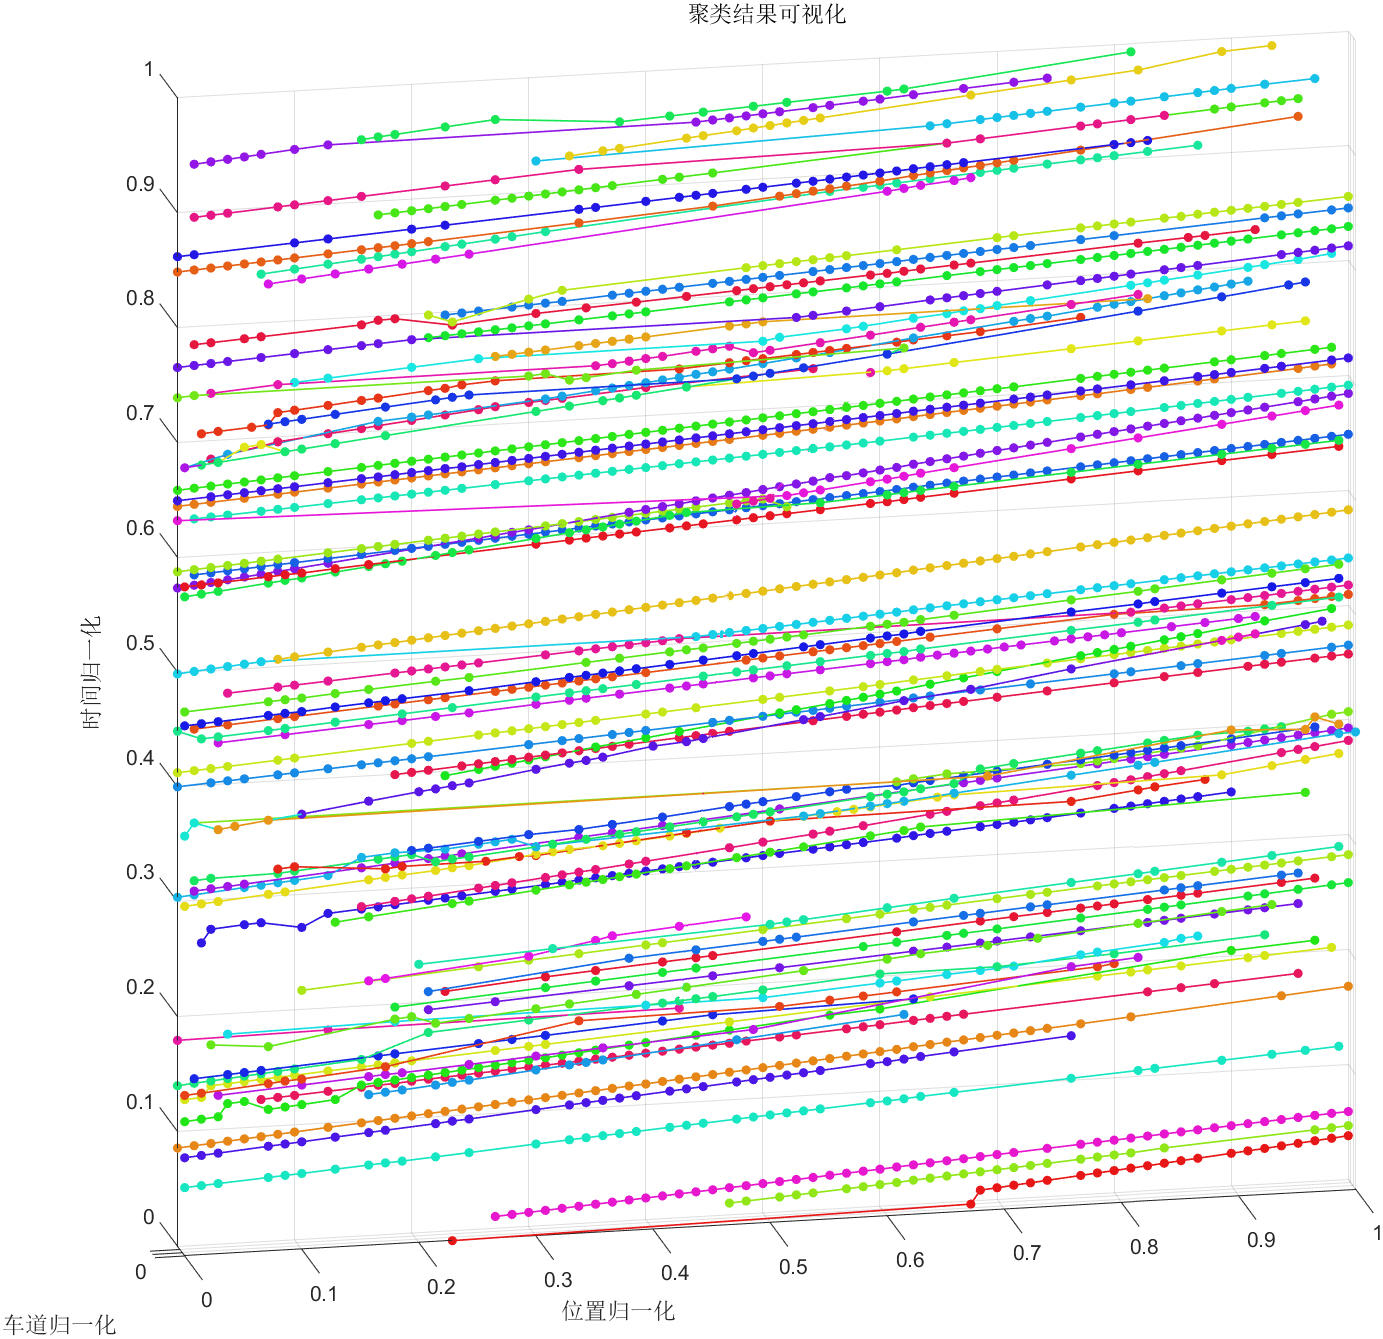
\includegraphics[width=0.72\textwidth]{images/chapter2/cluster_result.jpg}
	\caption{片段级在线聚类结果可视化}
	\label{fig:4_2_typical_case}
\end{figure}

图~\ref{fig:4_2_typical_case} 给出了本文方法在主场景下的片段级在线聚类结果可视化。图中以归一化后的位置、车道和时间作为三维坐标轴，不同颜色的点线对应不同的轨迹簇。可以看到，大多数片段在三维时空空间中能够沿车辆真实行驶方向形成连续、清晰且相互分离的聚类结构，说明本文方法能够将长缺测后原本碎片化的轨迹片段有效归并为较完整的车辆轨迹。对于局部邻近或存在交叠趋势的片段，聚类结果仍保持了较好的区分度，这表明方向约束与地磁辅助信息能够共同抑制明显的误拼接。

进一步地，图~\ref{fig:4_3_length_distribution} 给出了重构前后轨迹长度分布。可以看到，重构前分布主要集中在较短片段区间，而重构后分布整体向较长轨迹方向移动，短片段数量明显减少。这一现象与表~\ref{tab:4_2_overall_metrics} 中 $\mathrm{Frag}_{\mathrm{drop}}$ 的提升相一致，进一步说明本文方法能够有效降低第三章输出中的碎片化程度。综合表~\ref{tab:4_2_overall_metrics} 与图~\ref{fig:4_2_typical_case}、图~\ref{fig:4_3_length_distribution} 可知，第四章方法在总体重构质量上具有明显优势。



\begin{figure}[htbp]
	\centering
	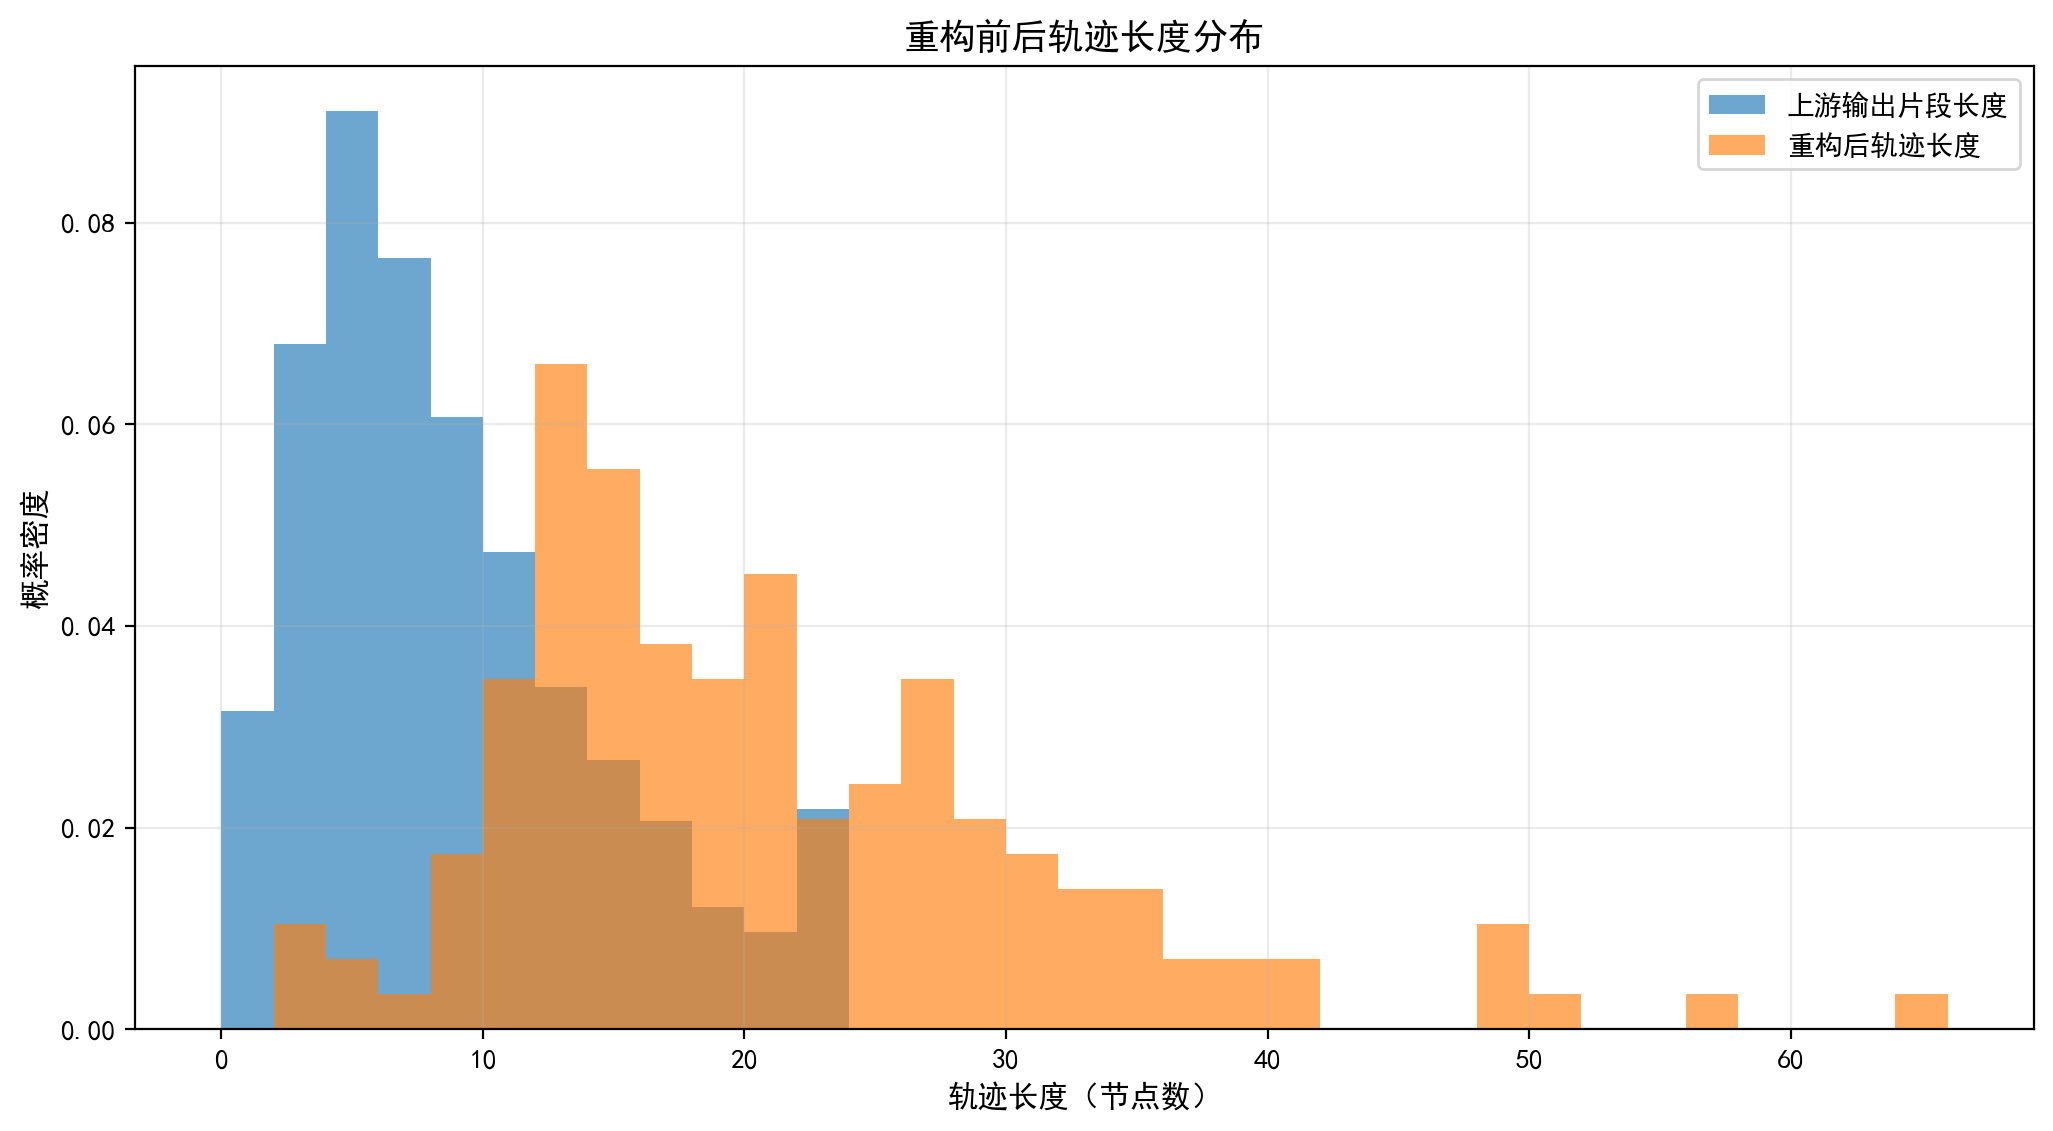
\includegraphics[width=0.82\textwidth]{fig_4_3_length_distribution.png}
	\caption{重构前后轨迹长度分布对比}
	\label{fig:4_3_length_distribution}
\end{figure}

\subsection{不同缺测强度下的性能分析}

长缺测强度实验用于分析本文方法在不同总体漏检率 $\eta_{\mathrm{miss}}$ 与最大连续缺测长度 $L_{\mathrm{miss}}$ 条件下的稳定性与适用边界。表~\ref{tab:4_3_tolerance_boundary} 给出了在满足 $F1_{\mathrm{link}}\ge 0.8$ 且 $R_{\mathrm{wm}}\le 0.1$ 条件时，两类方法可容忍的最大连续缺测长度。

\begin{table}[htbp]
	\centering
	\caption{不同总体漏检率下可容忍的最大连续缺测长度}
	\label{tab:4_3_tolerance_boundary}
	\begin{tabular}{lcccccc}
		\toprule
		方法 & $\eta_{\mathrm{miss}}=0.1$ & 0.2 & 0.3 & 0.4 & 0.5 & 0.6 \\
		\midrule
		仅上游样本输出 & 0 & 0 & 0 & 0 & 0 & 0 \\
		本文方法       & 3 & 5 & 6 & 6 & 6 & 6 \\
		\bottomrule
	\end{tabular}
\end{table}

由表~\ref{tab:4_3_tolerance_boundary} 可见，仅依赖上游样本输出的方法在所有漏检率条件下均无法满足有效重构要求；相比之下，本文方法在 $\eta_{\mathrm{miss}}=0.1$ 时即可容忍长度为 3 的连续缺测，在 $\eta_{\mathrm{miss}}\ge 0.3$ 时，可容忍的最大连续缺测长度进一步扩展到 6。该结果说明，本文提出的片段级在线聚类与轨迹重构方法显著拓展了系统对长缺测片段的可恢复边界。

图~\ref{fig:4_4_f1_vs_miss} 展示了总体漏检率变化对片段拼接 $F1$ 值的影响。可以看到，仅上游样本输出在各个漏检率水平上几乎均无法产生有效重构结果；而本文方法在 $\eta_{\mathrm{miss}}$ 从 0.1 增加到 0.6 的过程中，$F1_{\mathrm{link}}$ 仍维持在较高水平，说明该方法对总体漏检率变化具有较强适应性。需要指出的是，在当前样本流设置下，曲线并未呈现严格单调下降趋势，这表明最终拼接性能不仅受总体漏检比例影响，还与候选片段密度、时间重叠范围以及局部冲突强度等因素共同相关。

\begin{figure}[htbp]
	\centering
	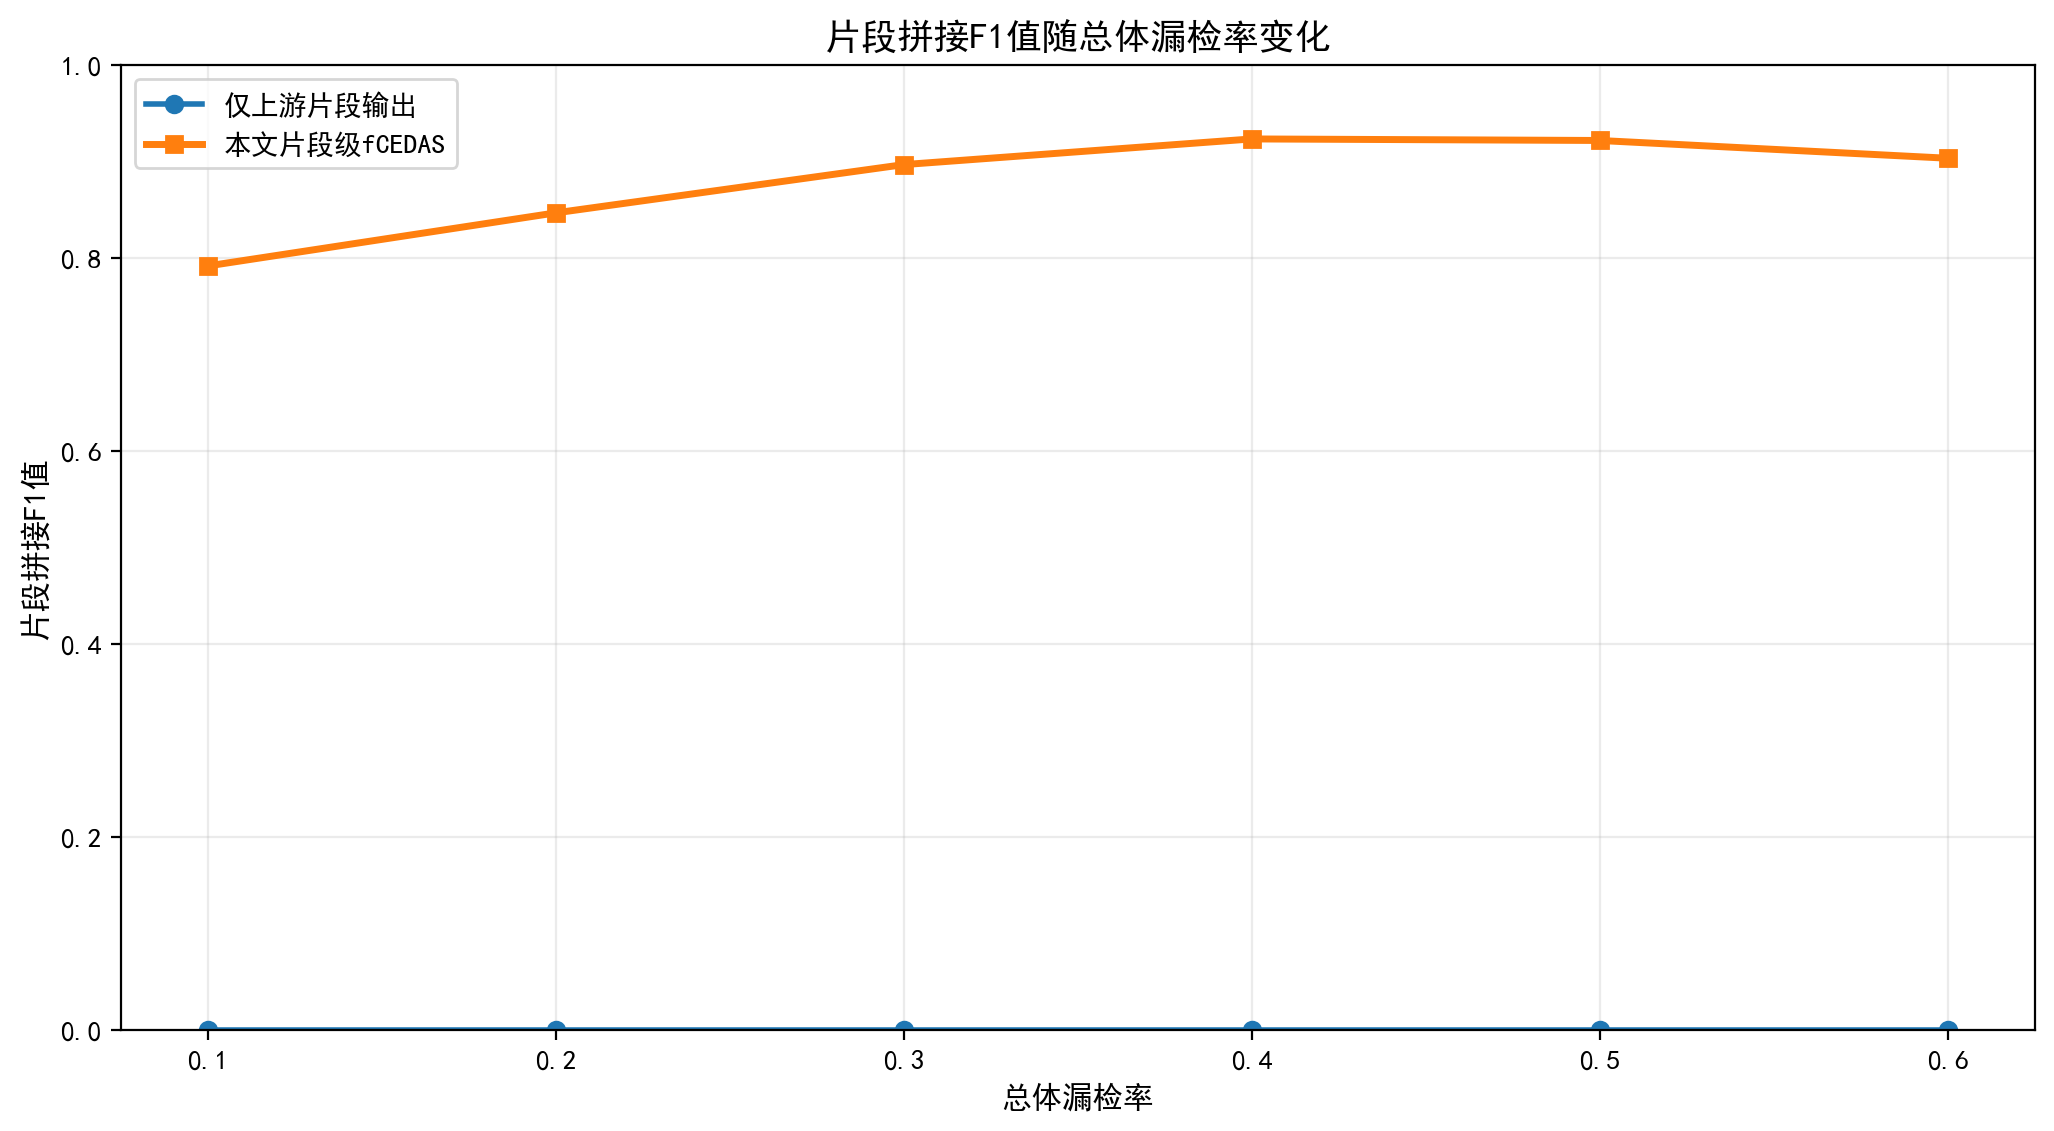
\includegraphics[width=0.82\textwidth]{fig_4_4_f1_vs_miss.png}
	\caption{片段拼接 $F1$ 值随总体漏检率变化}
	\label{fig:4_4_f1_vs_miss}
\end{figure}

图~\ref{fig:4_5_f1_vs_lmiss} 给出了最大连续缺测长度 $L_{\mathrm{miss}}$ 对 $F1_{\mathrm{link}}$ 的影响规律。总体来看，随着连续缺测长度增加，本文方法的拼接性能呈缓慢下降趋势，但即使在 $L_{\mathrm{miss}}=6$ 时，仍能够保持较高的 $F1$ 水平。这说明本文方法不仅适用于轻度缺测场景，也能够在较长连续缺测条件下维持可接受的重构质量。

\begin{figure}[htbp]
	\centering
	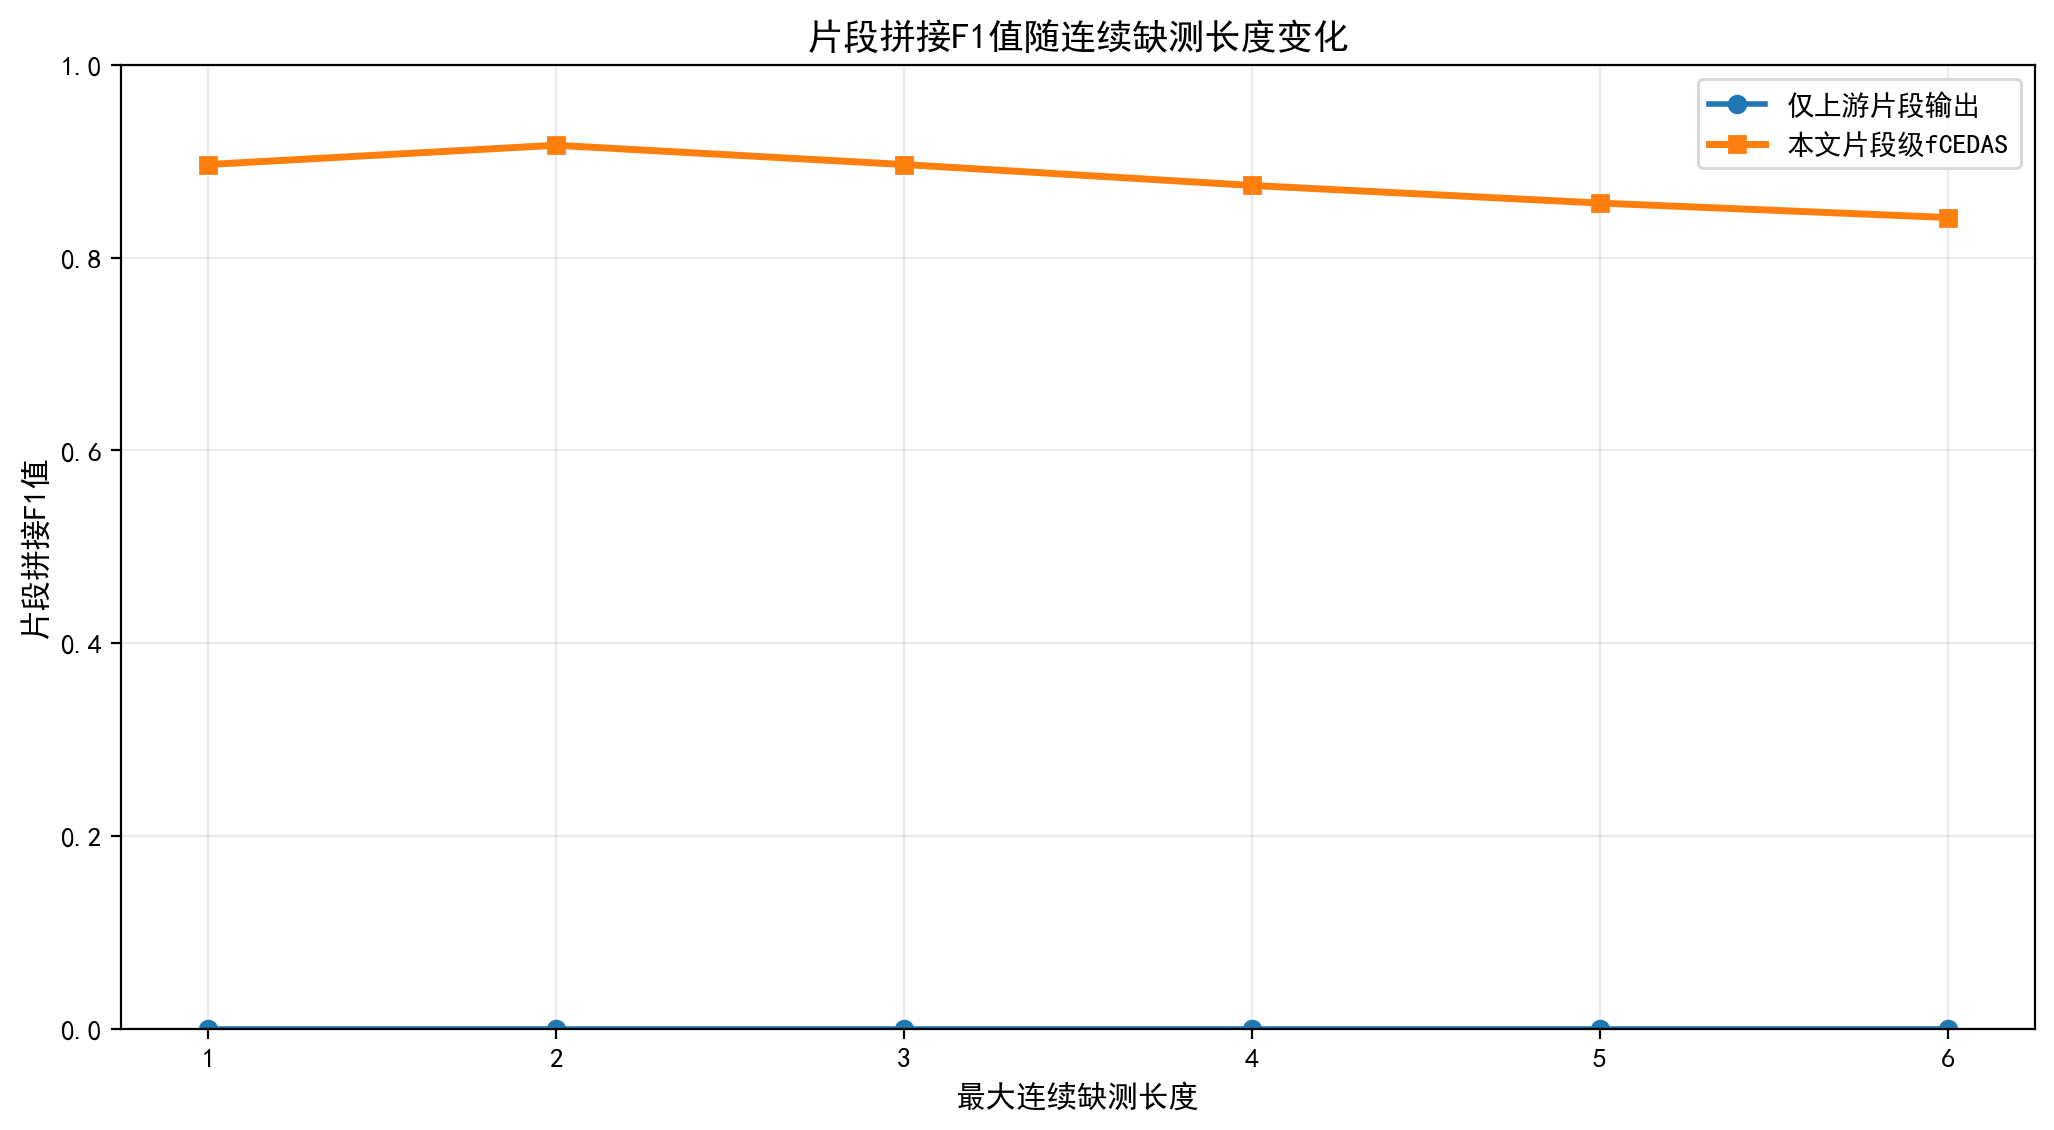
\includegraphics[width=0.82\textwidth]{fig_4_5_f1_vs_lmiss.png}
	\caption{片段拼接 $F1$ 值随最大连续缺测长度变化}
	\label{fig:4_5_f1_vs_lmiss}
\end{figure}

进一步地，图~\ref{fig:4_6_heatmap_full} 从二维视角刻画了 $\eta_{\mathrm{miss}}$ 与 $L_{\mathrm{miss}}$ 的耦合影响。结合热力图可知，在较大范围的长缺测强度条件下，本文方法的 $F1_{\mathrm{link}}$ 仍能维持在较高区间，说明其并非只在低缺测条件下有效，而是在中等到较高强度的长缺测场景中均表现出较好的鲁棒性。综合表~\ref{tab:4_3_tolerance_boundary} 与图~\ref{fig:4_4_f1_vs_miss} 至图~\ref{fig:4_6_heatmap_full} 可以认为，本文方法显著增强了系统对连续缺测场景的容忍能力。

\begin{figure}[htbp]
	\centering
	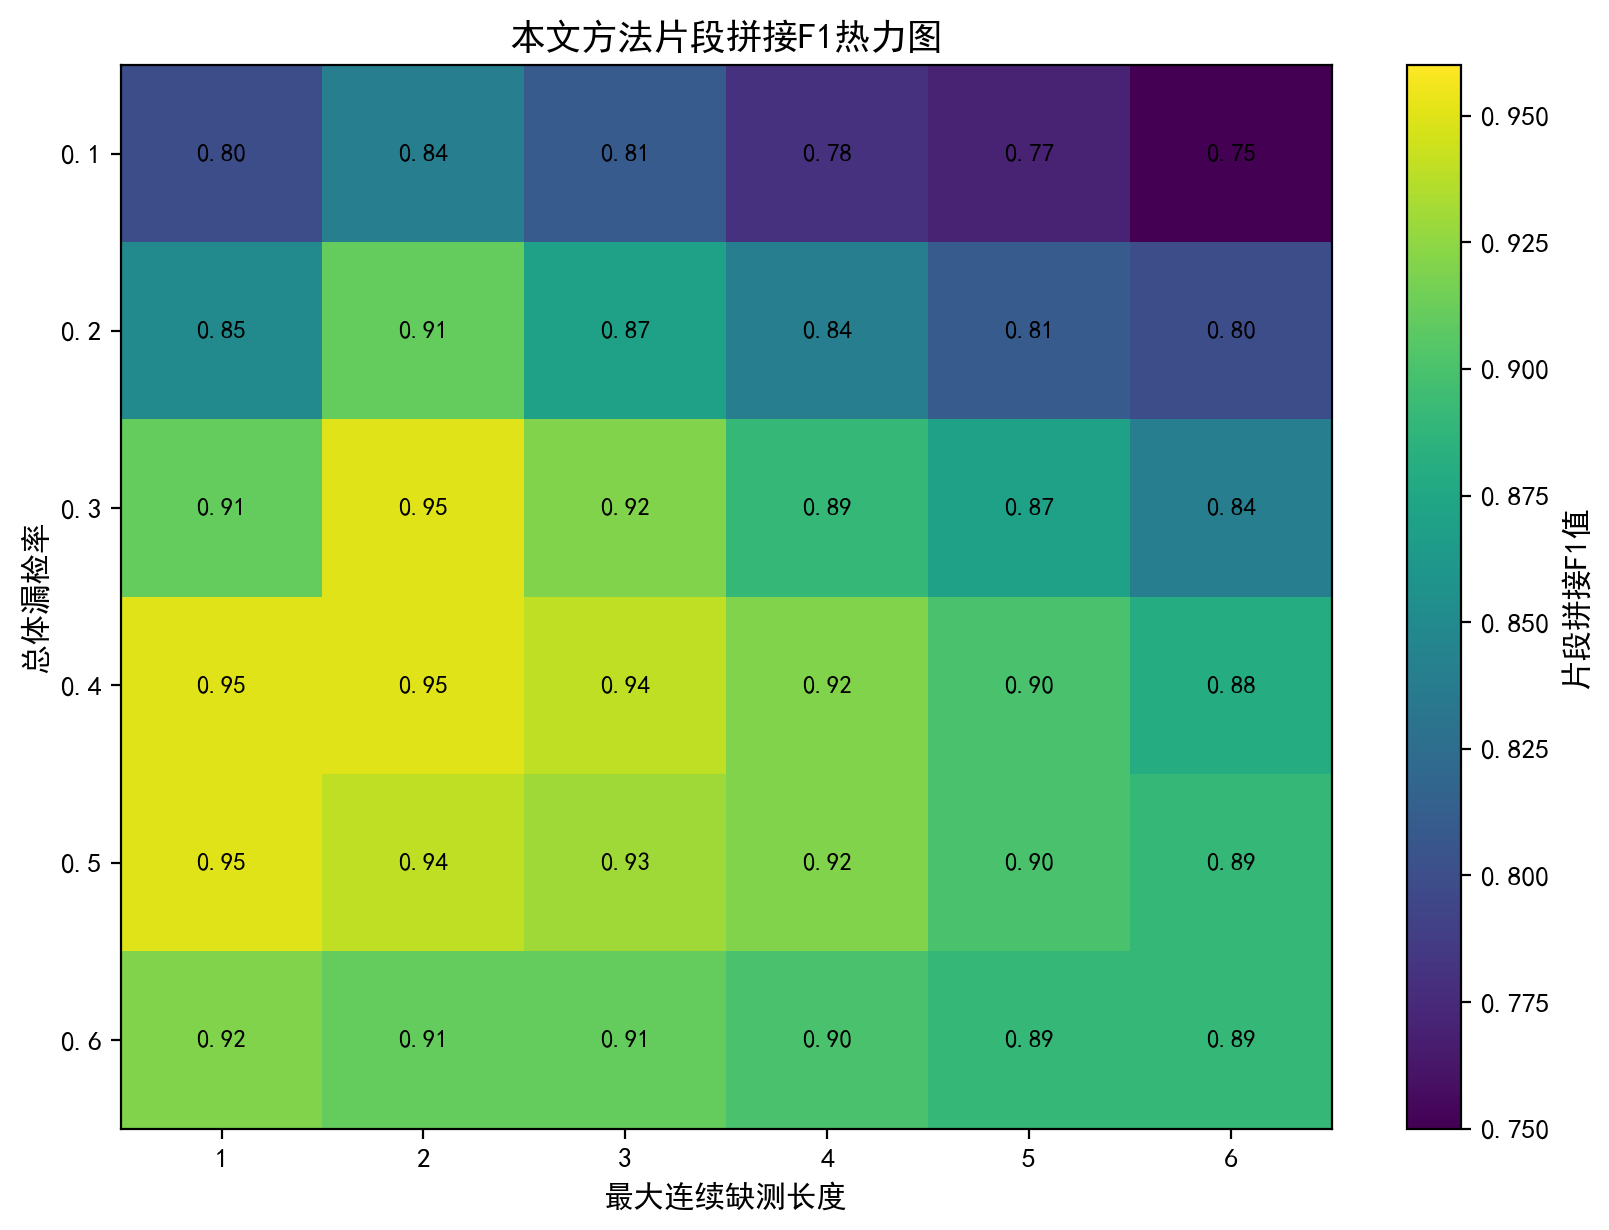
\includegraphics[width=0.88\textwidth]{fig_4_6_heatmap_full.png}
	\caption{不同漏检率与连续缺测长度下的片段拼接性能热力图}
	\label{fig:4_6_heatmap_full}
\end{figure}

\subsection{关键机制消融分析}

为进一步分析第四章方法中各关键环节的作用，本文设计了关键机制消融实验。考虑到第四章的主线是“方向主导、地磁辅助、簇尾摘要在线更新”，本节重点考察磁特征归一化、磁特征项、簇尾摘要更新方式等因素对最终重构性能的影响。同时，考虑到第四章以第三章输出为输入，本节也补充给出了去掉固定滞后重放的联动对比，用于说明上游片段质量变化对下游重构的影响。需要指出的是，这一联动对比并不改变第四章的方法主线，它只是用来说明两级处理框架之间的配合作用。

表~\ref{tab:4_4_ablation} 给出了完整方法及若干典型变体的对比结果。整体来看，完整方法在片段拼接 $F1$ 值、错并率、碎片消减量和重构召回率之间取得了更均衡的结果。

\begin{table}[htbp]
	\centering
	\caption{关键机制消融结果对比}
	\label{tab:4_4_ablation}
	\resizebox{0.86\textwidth}{!}{
		\begin{tabular}{lcccc}
			\toprule
			版本 & $F1_{\mathrm{link}}$ & $R_{\mathrm{wm}}$ & $\mathrm{Frag}_{\mathrm{drop}}$ & $R_{\mathrm{rec}}$ \\
			\midrule
			完整方法           & \textbf{0.8724} & 0.0476 & 343.000 & 0.8041 \\
			去掉磁特征归一化   & 0.8599 & \textbf{0.0464} & 335.125 & 0.7858 \\
			去掉磁特征项       & 0.7960 & 0.1379 & 317.000 & 0.7436 \\
			尾端直接覆盖       & 0.8704 & 0.0509 & \textbf{343.875} & \textbf{0.8063} \\
			去掉固定滞后重放   & 0.8607 & 0.0453 & 333.375 & 0.7817 \\
			保守更新           & 0.8674 & 0.0526 & 341.625 & 0.8006 \\
			\bottomrule
	\end{tabular}}
\end{table}

从表~\ref{tab:4_4_ablation} 可见，去掉磁特征项后，$F1_{\mathrm{link}}$ 由 0.8724 显著下降至 0.7960，同时错并率 $R_{\mathrm{wm}}$ 由 0.0476 大幅上升至 0.1379，说明在方向相近的片段之间，地磁特征是抑制错误拼接的关键约束。相较之下，去掉磁特征归一化虽然没有造成如此剧烈的性能退化，但 $F1_{\mathrm{link}}$ 与 $R_{\mathrm{rec}}$ 仍明显下降，说明归一化处理对于减弱节点间系统偏差、提高片段间地磁可比性具有现实必要性。

\begin{figure}[htbp]
	\centering
	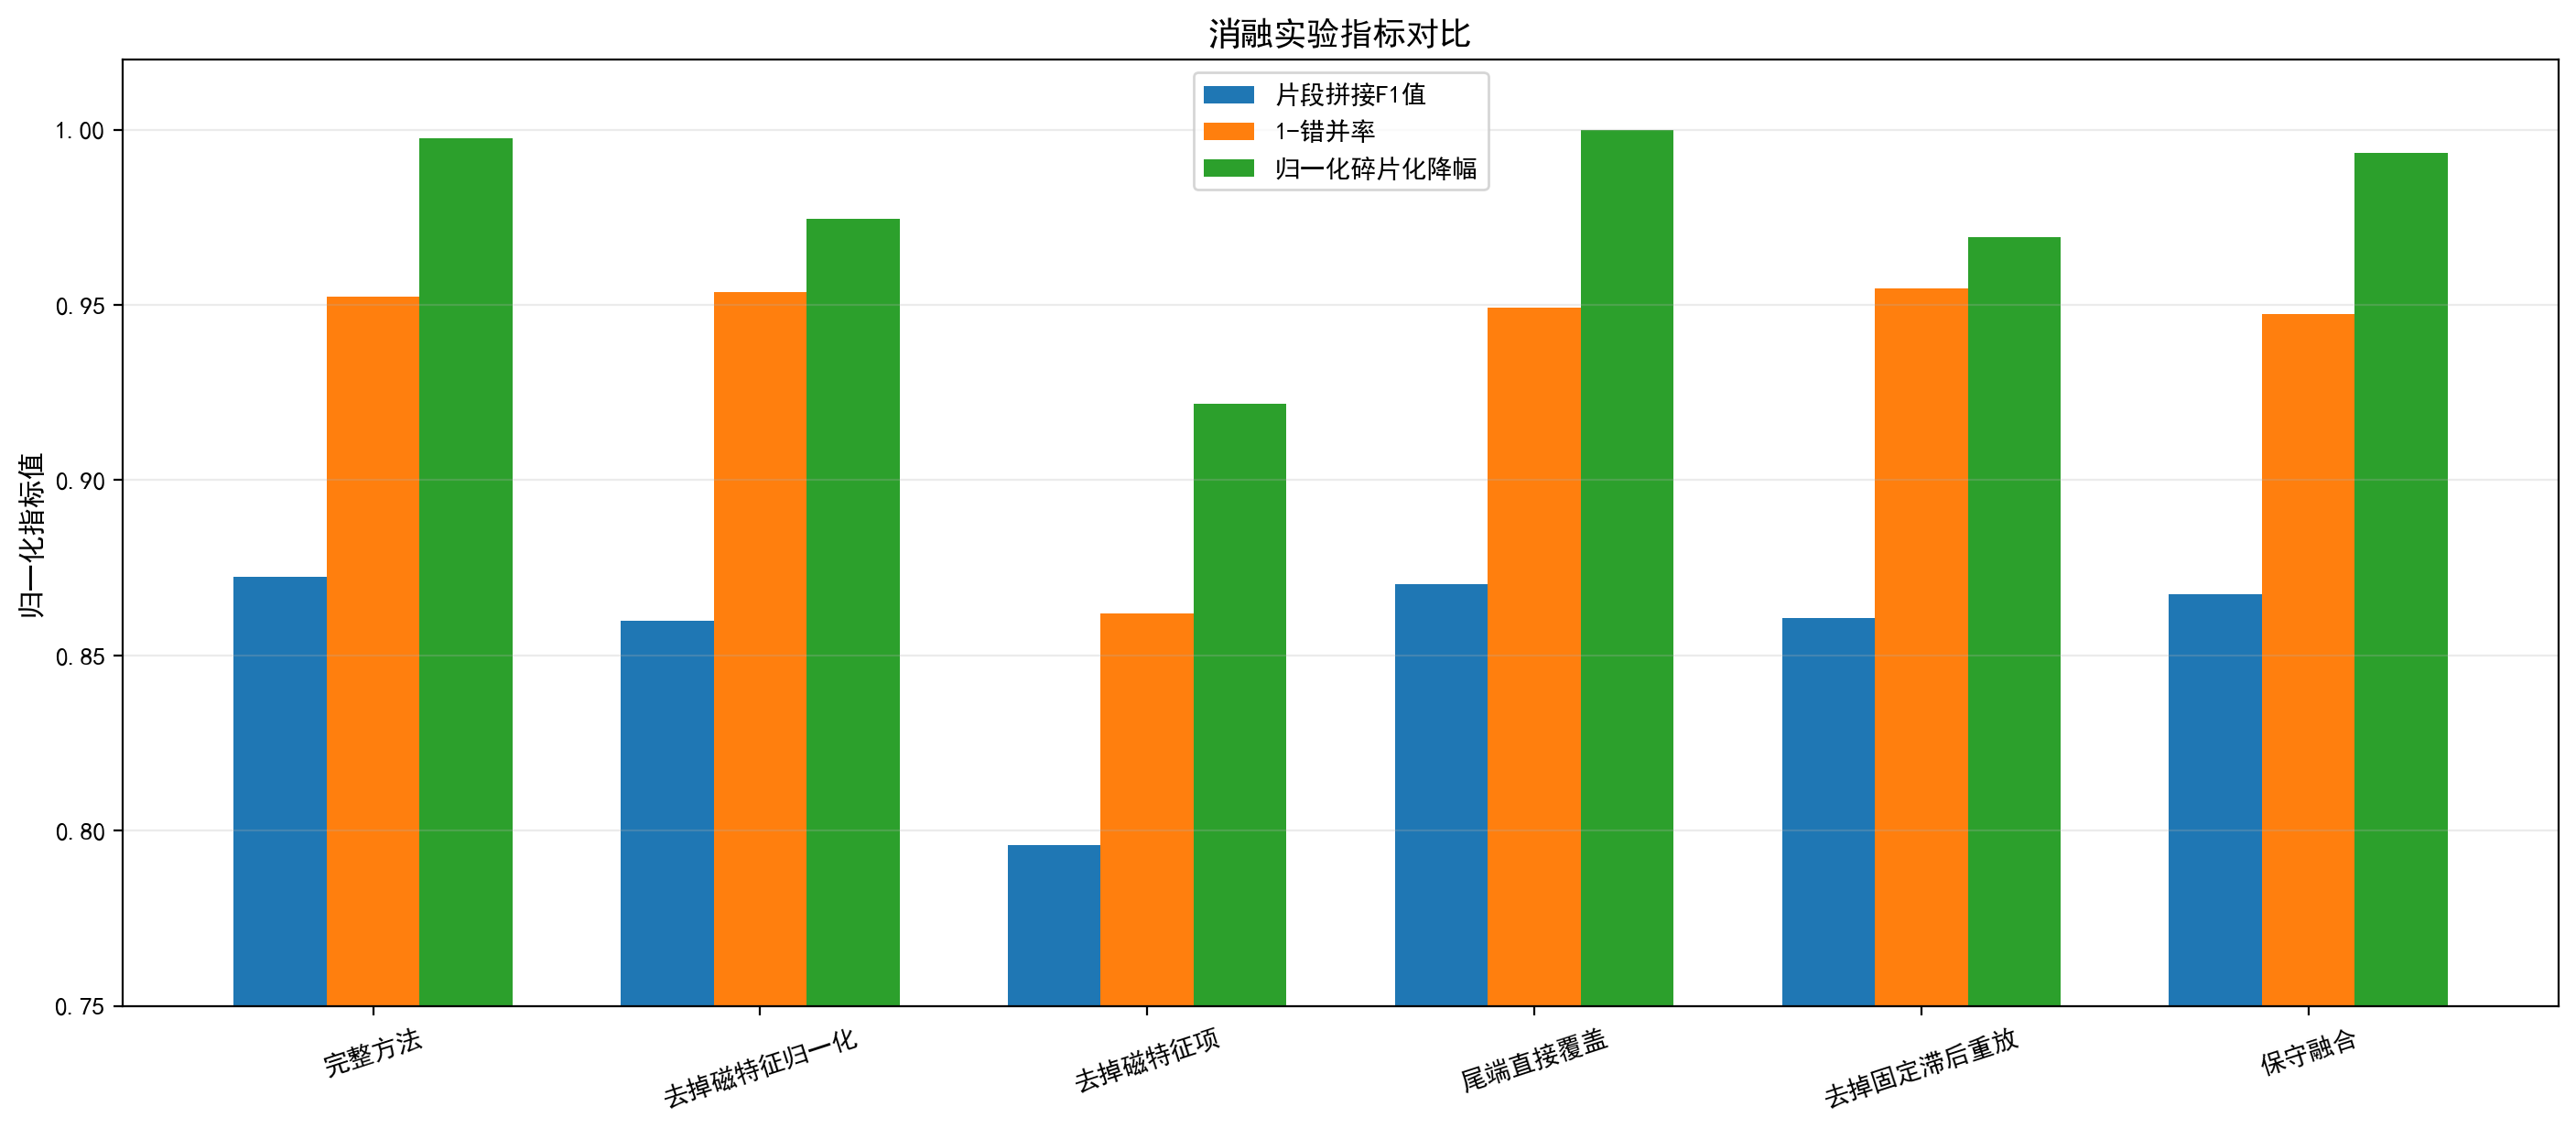
\includegraphics[width=0.88\textwidth]{fig_4_7_ablation_bar.png}
	\caption{关键机制消融结果对比}
	\label{fig:4_7_ablation_bar}
\end{figure}

图~\ref{fig:4_7_ablation_bar} 更直观地给出了不同变体在主要指标上的归一化结果。可以看到，完整方法在片段拼接质量、低错并率和碎片消减幅度三项指标之间取得了较好的平衡，而去掉磁特征项后的性能退化最为明显。这表明第四章虽然以方向约束作为主干，但如果缺少地磁辅助消歧，仅依赖方向一致性仍不足以支撑高质量的长缺测片段拼接。

\begin{figure}[htbp]
	\centering
	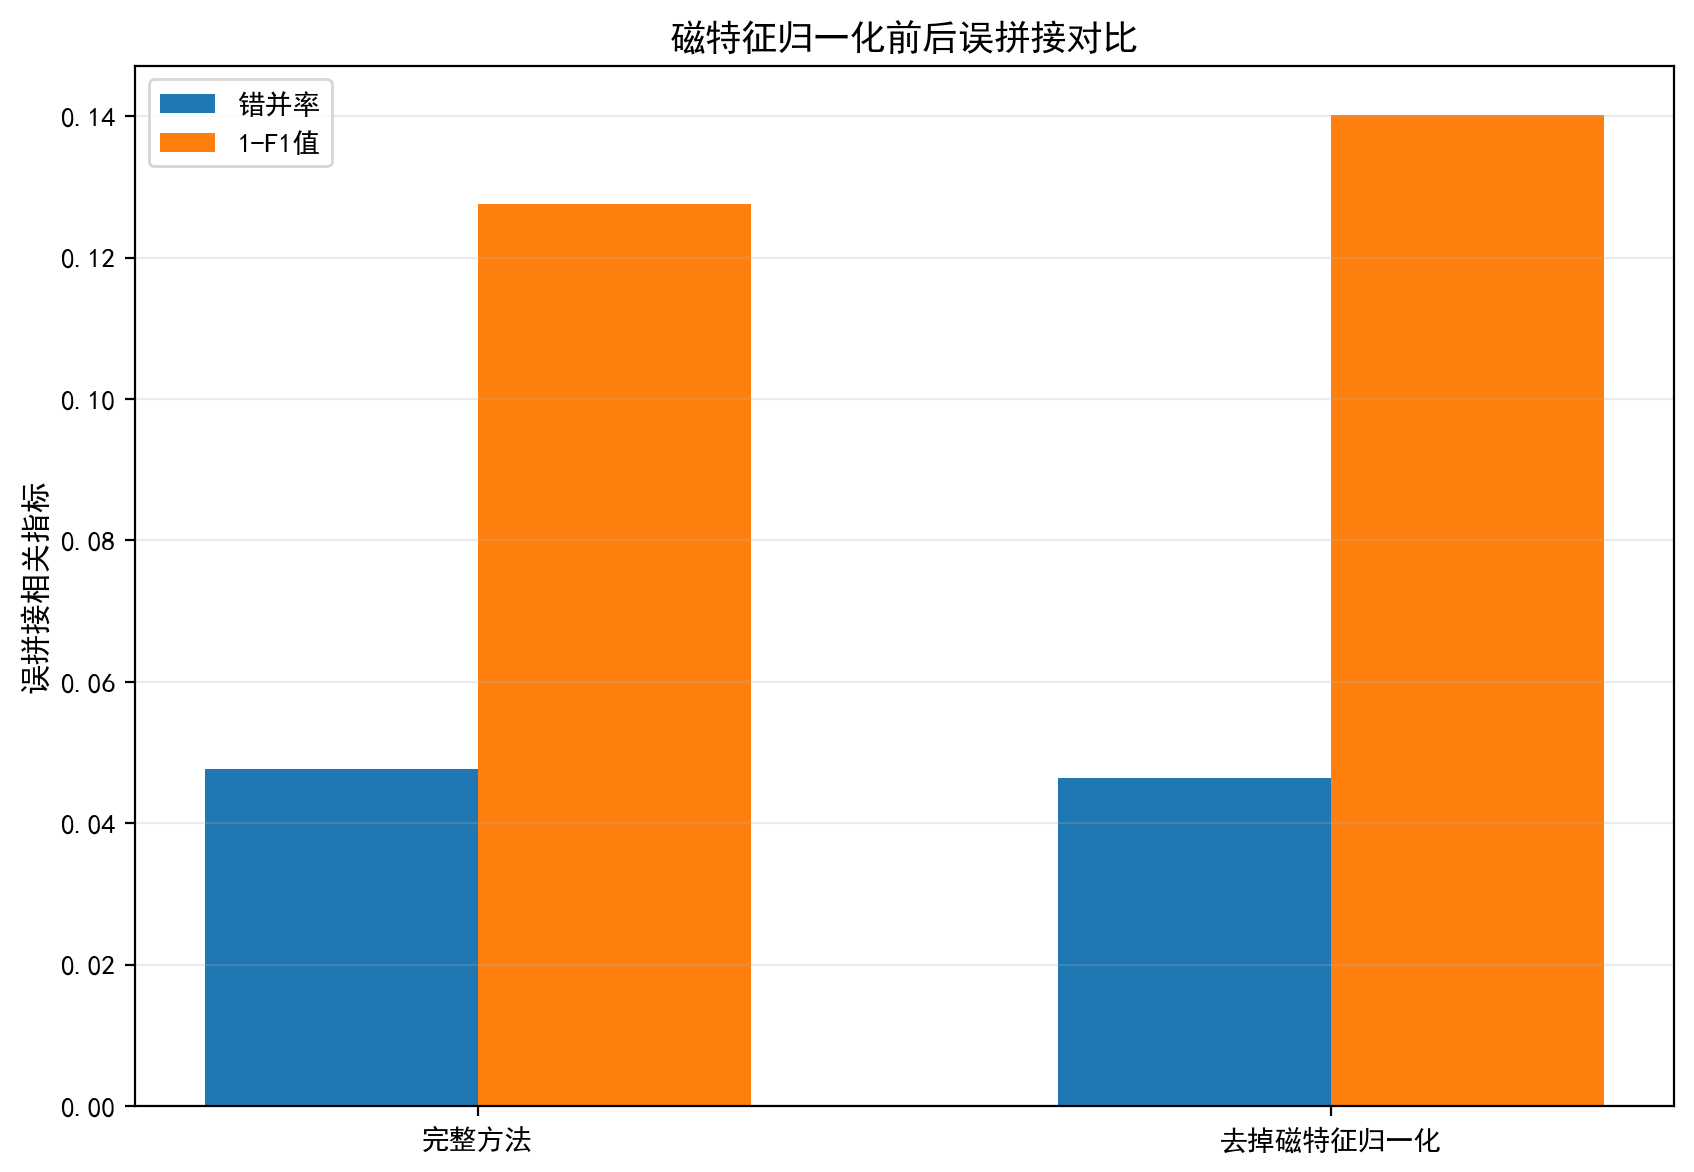
\includegraphics[width=0.74\textwidth]{fig_4_8_mag_norm_compare.png}
	\caption{地磁归一化前后重构效果对比}
	\label{fig:4_8_mag_norm_compare}
\end{figure}

图~\ref{fig:4_8_mag_norm_compare} 进一步比较了完整方法与“去掉磁特征归一化”变体在误拼接相关指标上的差异。可以看到，未进行归一化时，虽然错并率变化幅度有限，但整体 $F1_{\mathrm{link}}$ 和重构召回率都出现了明显下降。这说明未经归一化的地磁特征会把节点间的系统偏差直接带入拼接阶段，进而削弱地磁项在片段归并中的稳定作用。因此，地磁归一化并不是额外附加的装饰步骤，而是地磁信息能够稳定参与聚类评分的必要前提。

对于簇尾摘要更新方式，图~\ref{fig:4_9_fusion_compare} 给出了几种代表性更新策略的对比结果。结果表明，尾端直接覆盖的策略在碎片消减量和重构召回率上略占优势，但同时也带来了更高的错并风险；保守更新策略虽然更稳健，但整体 $F1_{\mathrm{link}}$ 略低于完整方法。相比之下，本文采用的支持度加权更新在重构质量、错并控制和稳定性之间取得了更均衡的结果，这与第四章方法的设计目标是一致的。

\begin{figure}[htbp]
	\centering
	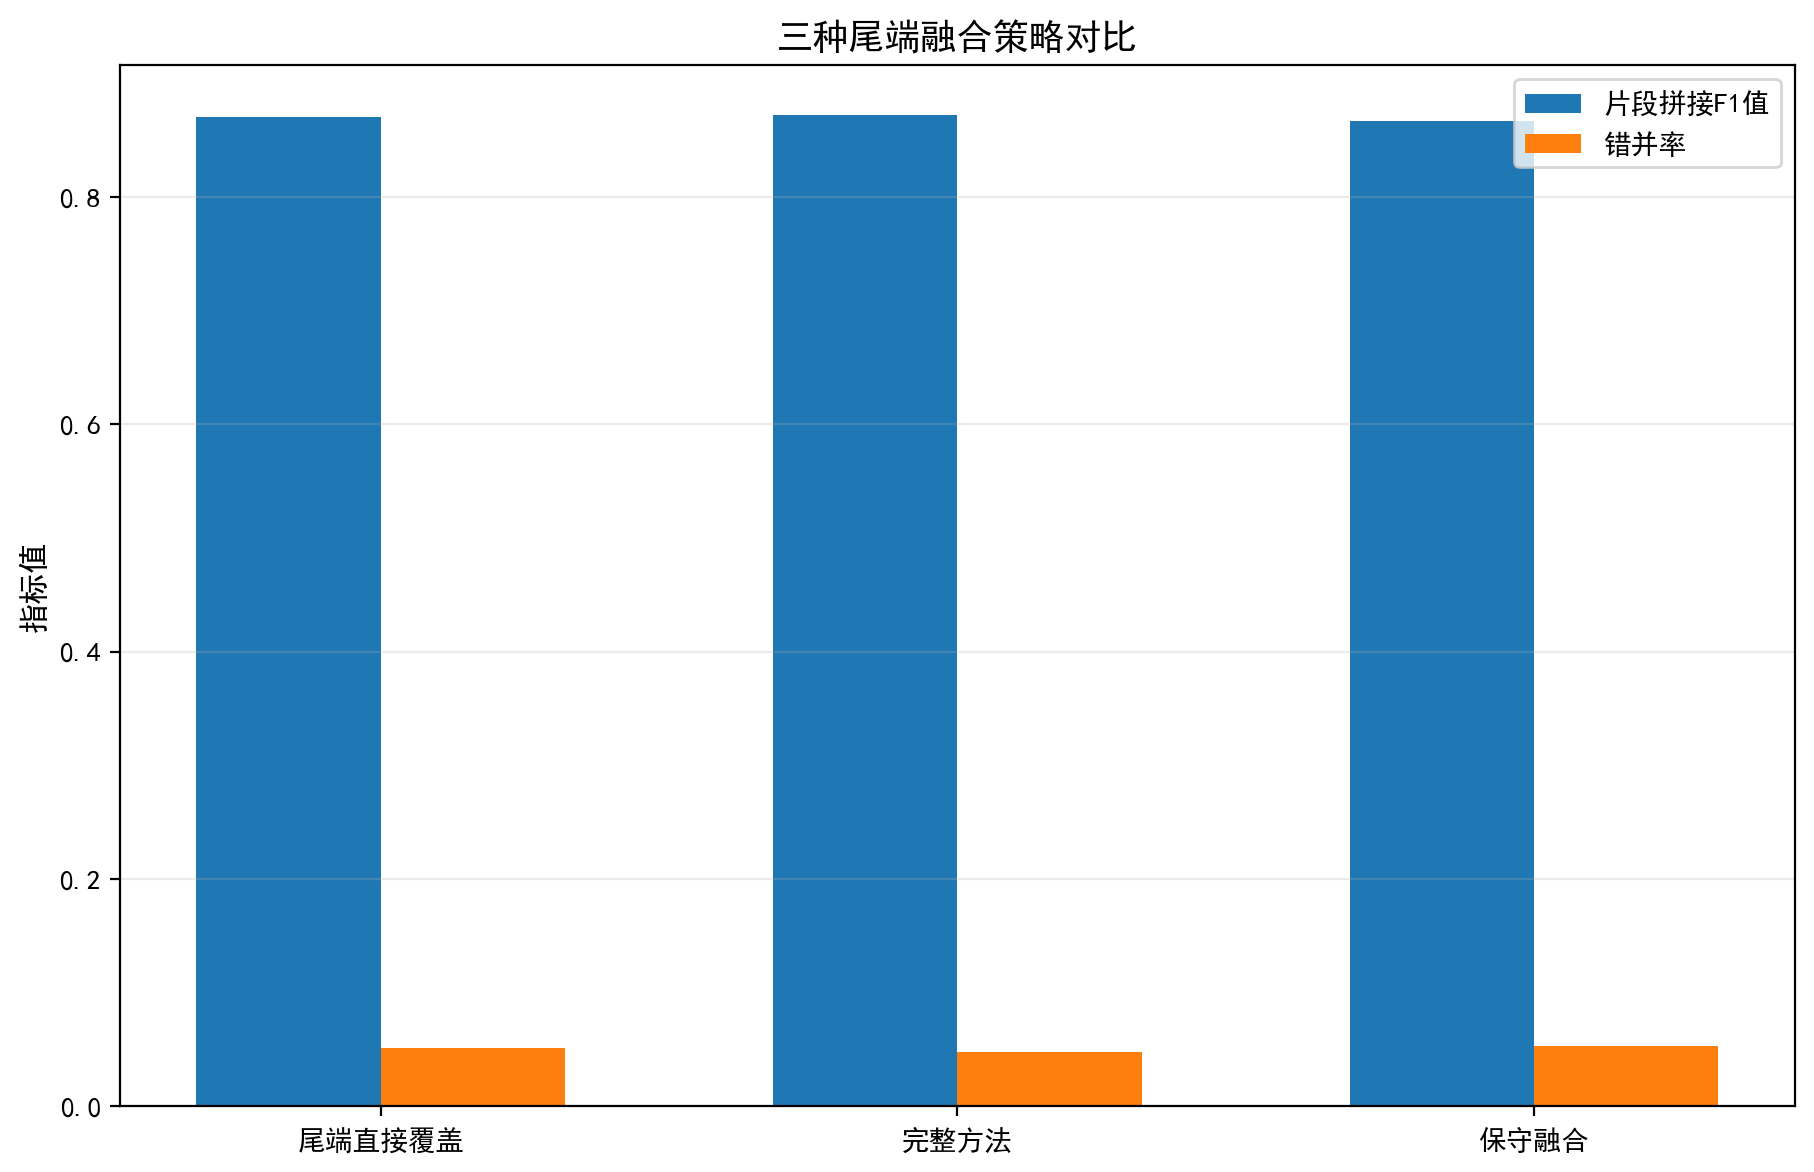
\includegraphics[width=0.74\textwidth]{fig_4_9_fusion_compare.png}
	\caption{不同簇尾摘要更新策略对比}
	\label{fig:4_9_fusion_compare}
\end{figure}

此外，去掉固定滞后重放后，虽然第四章的聚类评分形式并没有改变，但输入片段的质量与完整性下降，最终 $F1_{\mathrm{link}}$ 和 $R_{\mathrm{rec}}$ 也随之减小。这表明第四章与第三章在整体框架中是前后衔接、相互配合的关系。第三章负责尽量输出更完整、更可靠的片段流，第四章则在此基础上完成长缺测后的后验修复。综合表~\ref{tab:4_4_ablation} 与图~\ref{fig:4_7_ablation_bar} 至图~\ref{fig:4_9_fusion_compare} 可以看出，第四章方法的有效性并不是依赖某一个单独模块，而是方向约束、地磁辅助、地磁归一化、簇尾摘要更新以及上游输出质量共同作用的结果。

\section{本章小结}

本章针对系统长期运行后因传感器老化、检测能力下降以及复杂交通工况共同作用而引发的长缺测轨迹碎片化问题，在第三章上游在线跟踪结果基础上，提出了一种面向长缺测工况的片段级在线聚类与轨迹重构方法。与第三章面向事件级在线跟踪的处理对象不同，第四章不再围绕点级状态递推展开，而是将上游输出的轨迹片段及未得到关联的单点量测统一表示为片段样本，并据此构建簇图结构与簇尾摘要。

在方法设计上，本文将片段压缩表示为“方向向量、地磁代表值、支持度和起止时间戳”，从而以尽可能少的变量保留轨迹重构所需的关键信息；随后，围绕簇初始化、融合方向约束的聚类相似度评分计算、簇尾摘要更新以及生命周期管理等关键环节，建立了完整的在线聚类与轨迹重构流程。与将第四章写成状态传播和不确定度递推框架的做法相比，这一写法更贴近会议论文的原始思路，也更符合本章作为片段级后验修复模块的定位。

实验结果表明，所提方法能够有效恢复长缺测后断裂的车辆轨迹，降低错误拼接和身份切换，并在中等至较高缺测强度范围内保持较稳定的片段拼接性能。综合来看，基于簇图结构与聚类相似度评分的片段级在线聚类方法，为多地磁传感器系统在长期运行条件下的轨迹重构提供了一条清晰、可实现且与会议论文思路一致的技术路径。





\chapter{总结与展望}

\section{总结}

本文围绕单向双车道高速公路场景下的多地磁传感器车辆目标跟踪问题开展研究，针对量测乱序、短时漏检、噪声干扰、邻道干扰与双车并行易混淆，以及长期运行后传感器退化引起的长缺测和轨迹碎片化等问题，构建了“事件级在线跟踪—片段级在线重构”的两级处理框架。本文的主要创新在于，将固定滞后回放、节点状态自适应和场景概率判别统一到事件级在线跟踪过程中，并进一步提出面向长缺测的片段级在线聚类与轨迹重构方法，使常态工况跟踪与长缺测修复能够前后衔接。

在在线跟踪层面，本文提出了基于节点状态自适应与场景概率判别的多车辆跟踪方法。该方法通过时间窗口缓存和固定滞后回放处理迟到量测，在事件级状态估计的基础上，将节点检测概率、杂波强度与场景后验共同引入数据关联和轨迹管理过程，从而提升了复杂工况下的关联稳定性和车道判别能力。实验结果表明，在困难并行场景下，场景判别准确率提升至 $0.9262$；在常规车流条件下，系统可较稳定地容忍连续 $2\sim3$ 个地磁传感器漏检，在低密度条件下可扩展至连续 $3\sim4$ 个；当固定滞后窗口长度取 $L=4$ 时，迟到量测吸收比例达到 $0.7194$，在线与离线结果一致率达到 $0.7064$。这说明所提方法能够较好适应双车道高速场景下多地磁事件流的在线处理需求。

在长缺测重构层面，本文进一步提出了面向长缺测工况的片段级在线聚类与轨迹重构方法。该方法以第三章输出的轨迹片段和未关联单点量测为输入，构建簇图结构，并融合方向约束、磁特征相似性、车道一致性和簇尾状态融合完成片段归并，在不回到原始点级量测的前提下实现对碎片化轨迹的后验修复。实验结果表明，相较于传统在线聚类基线，所提方法将片段拼接 $F1_{\mathrm{link}}$ 提升至 $0.8595$，将错并率降至 $0.0471$，并将身份切换次数由 $87$ 降至 $73$，FMI 提升至 $0.8015$。总体来看，本文形成了一套面向多地磁传感器车辆目标跟踪的完整处理链条，为高速公路运行监测和轨迹级交通分析提供了可行的方法支撑。

\section{未来展望}

本文的研究工作主要面向单向双车道高速公路场景展开，相关的场景建模、车道状态更新和并行场景判别都利用了该场景的结构先验。后续可进一步面向多车道高速、匝道汇入汇出区域以及更复杂的路段结构，研究更一般的场景表达和轨迹管理方法，以提升算法的泛化能力和适用范围。

此外，虽然本文已经对节点检测概率和杂波强度进行了在线自适应建模，但固定滞后窗口长度、门控阈值和片段聚类权重等参数仍存在一定经验依赖；同时，当前对地磁信息的利用仍以峰值等低维统计特征为主，对波形细节和多尺度特征的挖掘还不够充分。后续可进一步研究参数自整定方法以及更丰富的地磁特征表示，并将其与车辆运动状态、车道信息联合建模，以提升复杂干扰和高相似目标条件下的区分能力。

从工程应用角度看，后续还需要在更长时间跨度、更大部署范围和更多交通状态条件下对本文方法进行持续验证，并进一步优化在线计算复杂度与存储开销，增强其在边缘端或云边协同场景中的实时部署能力。若上述问题能够继续推进，多地磁传感器车辆目标跟踪方法有望在高速公路运行监测、交通安全分析和精细化管控中发挥更大作用。

\end{document}